%-----------------------------------------------------------------------
% Template File for Science China Information Sciences
% Converted from the IEEEtran survey by move-content conversion
%-----------------------------------------------------------------------
\documentclass{SCIS2026}

%%%%%%%%%%%%%%%%%%%%%%%%%%%%%%%%%%%%%%%%%%%%%%%%%%%%%%%
%%% Author's definitions for this manuscript
%%%%%%%%%%%%%%%%%%%%%%%%%%%%%%%%%%%%%%%%%%%%%%%%%%%%%%%
\usepackage[table,dvipsnames]{xcolor}
\usepackage{ragged2e}
\usepackage{makecell}
\usepackage{textcomp}
\usepackage{array}
\usepackage{amsmath}

% SCIS caption prefix is "Fig." (matches the in-text "Fig.~\ref{}" style)
\renewcommand{\figurename}{Fig.}

% 自动换行、右对齐，禁止自动缩进
\newcolumntype{Y}{>{\RaggedRight\arraybackslash}X}
\newcolumntype{L}[1]{>{\RaggedRight\arraybackslash}p{#1}}

% 行距与列间距
\renewcommand{\arraystretch}{1.45}
\setlength{\tabcolsep}{5pt}

% 表格分组命令
\newcommand{\evalgroup}[1]{%
    \rowcolor{TableSub}
    \multicolumn{5}{@{}l}{%
        \hspace{0.25em}\textcolor{TableNavy}{\bfseries #1}%
    }\\[-0.15em]%
}

%%% 颜色定义（CVPR 风格表头配色）%%%
\definecolor{TitleBlue}{HTML}{172C67}
\definecolor{LineBlue}{HTML}{AAB8E8}
\definecolor{BlueText}{HTML}{1E55B3}
\definecolor{GreenText}{HTML}{287B32}
\definecolor{OrangeText}{HTML}{EE6B19}
\definecolor{PurpleText}{HTML}{7040A7}
\definecolor{CyanText}{HTML}{13889A}
\definecolor{RedText}{HTML}{D52D35}
\definecolor{DeepBlueText}{HTML}{164D9B}
\definecolor{BlueBG}{HTML}{F5F8FF}
\definecolor{GreenBG}{HTML}{F5FAF4}
\definecolor{OrangeBG}{HTML}{FFF9F3}
\definecolor{PurpleBG}{HTML}{FAF7FD}
\definecolor{CyanBG}{HTML}{F3FAFC}
\definecolor{RedBG}{HTML}{FFF7F7}
\definecolor{HeaderBlue}{RGB}{24,62,130}
\definecolor{MethodGreen}{RGB}{0,110,80}
\definecolor{CapabilityBlue}{RGB}{35,75,170}
\definecolor{ChallengeRed}{RGB}{170,40,40}
\definecolor{LightGray}{RGB}{246,247,249}
\definecolor{lightBlue}{RGB}{220,235,255}

% === 第二个表格的颜色 ===
\definecolor{ChallengeBlue}{HTML}{183A85}
\definecolor{EssenceGreen}{HTML}{69B34C}
\definecolor{SolutionPurple}{HTML}{7052B8}
\definecolor{ChallengeBG}{HTML}{F6F8FD}
\definecolor{EssenceBG}{HTML}{F7FBF4}
\definecolor{SolutionBG}{HTML}{FAF8FD}
\definecolor{GoalBG}{HTML}{F8FAFE}
\definecolor{SolutionText}{HTML}{6943B5}

% === 表格颜色 ===
\definecolor{TableNavy}{HTML}{17324D}
\definecolor{TableBlue}{HTML}{DCE8F2}
\definecolor{TableSub}{HTML}{EEF3F7}
\definecolor{TableRule}{HTML}{8FA5B8}
\definecolor{GrayRule}{HTML}{C5C9CD}

% 标记符号
\definecolor{red}{RGB}{192,0,0}
\definecolor{green}{RGB}{0,176,80}
\definecolor{blue}{RGB}{0,112,192}
\newcommand{\cmark}{\ding{51}}
\newcommand{\xmark}{\ding{55}}
\newcommand{\noo}{\textcolor{red}{\xmark}}
\newcommand{\yes}{\textcolor{OliveGreen}{\checkmark}}

% ---------- 单元格命令 ----------
\newcommand{\CenterCell}[1]{%
    \begin{minipage}[t][2.55cm][t]{\linewidth}%
    \centering
    \vspace{0.05cm}
    #1
    \end{minipage}%
}

\newcommand{\LeftCell}[1]{%
    \begin{minipage}[t][2.55cm][t]{\linewidth}%
    \raggedright
    \vspace{0.05cm}
    #1
    \end{minipage}%
}

\newcommand{\CategoryCell}[1]{%
    \begin{minipage}[c]{\linewidth}%
    \raggedright
    \setlength{\parindent}{0pt}%
    \vspace*{1pt}%
    \noindent\ignorespaces#1\unskip\par
    \vspace*{1pt}%
    \end{minipage}%
}

\newcommand{\strength}[1]{\textcolor{BlueText}{\textbf{Strength: }}#1}
\newcommand{\limitation}[1]{\textcolor{GreenText}{\textbf{Limitation: }}#1}

\newcommand{\ChallengeCell}[1]{%
    \begin{minipage}[t][3.10cm][t]{\linewidth}%
    \centering
    \vspace{0.14cm}
    \textcolor{ChallengeBlue}{\bfseries #1}%
    \end{minipage}%
}

\newcommand{\EssenceCell}[1]{%
    \begin{minipage}[t][3.10cm][t]{\linewidth}%
    \raggedright
    \vspace{0.10cm}
    #1
    \end{minipage}%
}

\newcommand{\SolutionCell}[1]{%
    \begin{minipage}[t][3.10cm][t]{\linewidth}%
    \raggedright
    \vspace{0.10cm}
    #1
    \end{minipage}%
}

\newcommand{\solutionitem}[2]{\textcolor{SolutionText}{\bfseries #1: }#2}
\newcommand{\tablebullet}{\raisebox{0.15ex}{\scriptsize$\bullet$}\hspace{0.45em}}

%%%%%%%%%%%%%%%%%%%%%%%%%%%%%%%%%%%%%%%%%%%%%%%%%%%%%%%
%%% Begin.
%%%%%%%%%%%%%%%%%%%%%%%%%%%%%%%%%%%%%%%%%%%%%%%%%%%%%%%
\begin{document}

%%%%%%%%%%%%%%%%%%%%%%%%%%%%%%%%%%%%%%%%%%%%%%%%%%%%%%%
%%% Authors do not modify the information below
%%%%%%%%%%%%%%%%%%%%%%%%%%%%%%%%%%%%%%%%%%%%%%%%%%%%%%%
\ArticleType{REVIEW}
\Year{2026}
\Month{March}
\Vol{69}
\No{1}
\DOI{}
\ArtNo{}
\ReceiveDate{}
\ReviseDate{}
\AcceptDate{}
\OnlineDate{}
\AuthorMark{}
\AuthorCitation{}

%%% title
\title{Actionable Scene Understanding for Indoor Embodied Manipulation: A Survey}{Actionable Scene Understanding for Indoor Embodied Manipulation: A Survey}

%%% Corresponding author: name + {{email}}
%%% General author: name only
%%% Equal contribution: \dag in the affiliation list
%% Non-corresponding authors' student e-mails (from the IEEE source):
%%   Yaze Li 2024218446 / Xinyu Xie 2024218501 /
%%   Jiawei Ma 2024218545 / Siying Song 2024218492 @mail.hfut.edu.cn
\author[1\dag]{Yaze Li}{}
\author[1\dag]{Xinyu Xie}{}
\author[1\dag]{Jiawei Ma}{{jiawei@hfut.edu.cn}}
\author[1\dag]{Siying Song}{}
\author[2]{Jianan Zou}{{aujazou@mail.scut.edu.cn}}
\author[1]{Haihong Xiao}{{haihong@mail.hfut.edu.cn}}
\author[1]{Wei Jia}{}

%%% Authors' contribution
\contributions{Yaze Li, Xinyu Xie, Jiawei Ma and Siying Song contributed equally to this work.}

%%% Address
\address[1]{School of Computer Science and Information Engineering, Hefei University of Technology, Hefei, China}
\address[2]{School of Automation Science and Engineering, South China University of Technology, Guangzhou, China}

%%% Abstract
\abstract{Scene understanding for embodied manipulation must extend beyond describing what exists in an environment to representing what can be acted upon, under which physical constraints, and with what consequences. Existing surveys have largely examined geometric reconstruction, semantic understanding, functional reasoning, or embodied intelligence as separate research directions, leaving their roles in task-oriented behavior insufficiently characterized. This survey presents a unified perspective on \emph{actionable scene understanding} for embodied manipulation, where scene knowledge is organized according to its utility for task-conditioned perception, physical reasoning, prediction, and action. We distinguish conventional scene understanding, which primarily recovers geometric and semantic structure, from actionable scene understanding, which additionally incorporates functional affordances, physical properties and constraints, causal relations, and state evolution. From this perspective, we review datasets and evaluation protocols, geometric reconstruction, semantic understanding, physical and functional understanding, and embodied scene modeling, while examining the gap between perceptual fidelity and executable behavior. We further identify emerging directions toward latent physical-state inference, interaction-driven scene updating, persistent predictive scene modeling, and human-aware embodied understanding. By connecting scene representation with action-conditioned prediction and closed-loop behavior, this survey aims to provide a systematic view of how 3D scene understanding can evolve from descriptive reconstruction toward executable scene knowledge.\ Project page: \url{https://saltgardenia.github.io/Actionable-Scene-Understanding/}.}

%%% Keywords
\keywords{spatial intelligence, world models, embodied manipulation, 3D scene understanding, affordance reasoning}

\maketitle

%%%%%%%%%%%%%%%%%%%%%%%%%%%%%%%%%%%%%%%%%%%%%%%%%%%%%%%
%%% The main text.
%%%%%%%%%%%%%%%%%%%%%%%%%%%%%%%%%%%%%%%%%%%%%%%%%%%%%%%
\begin{figure}[!t]
    \centering
    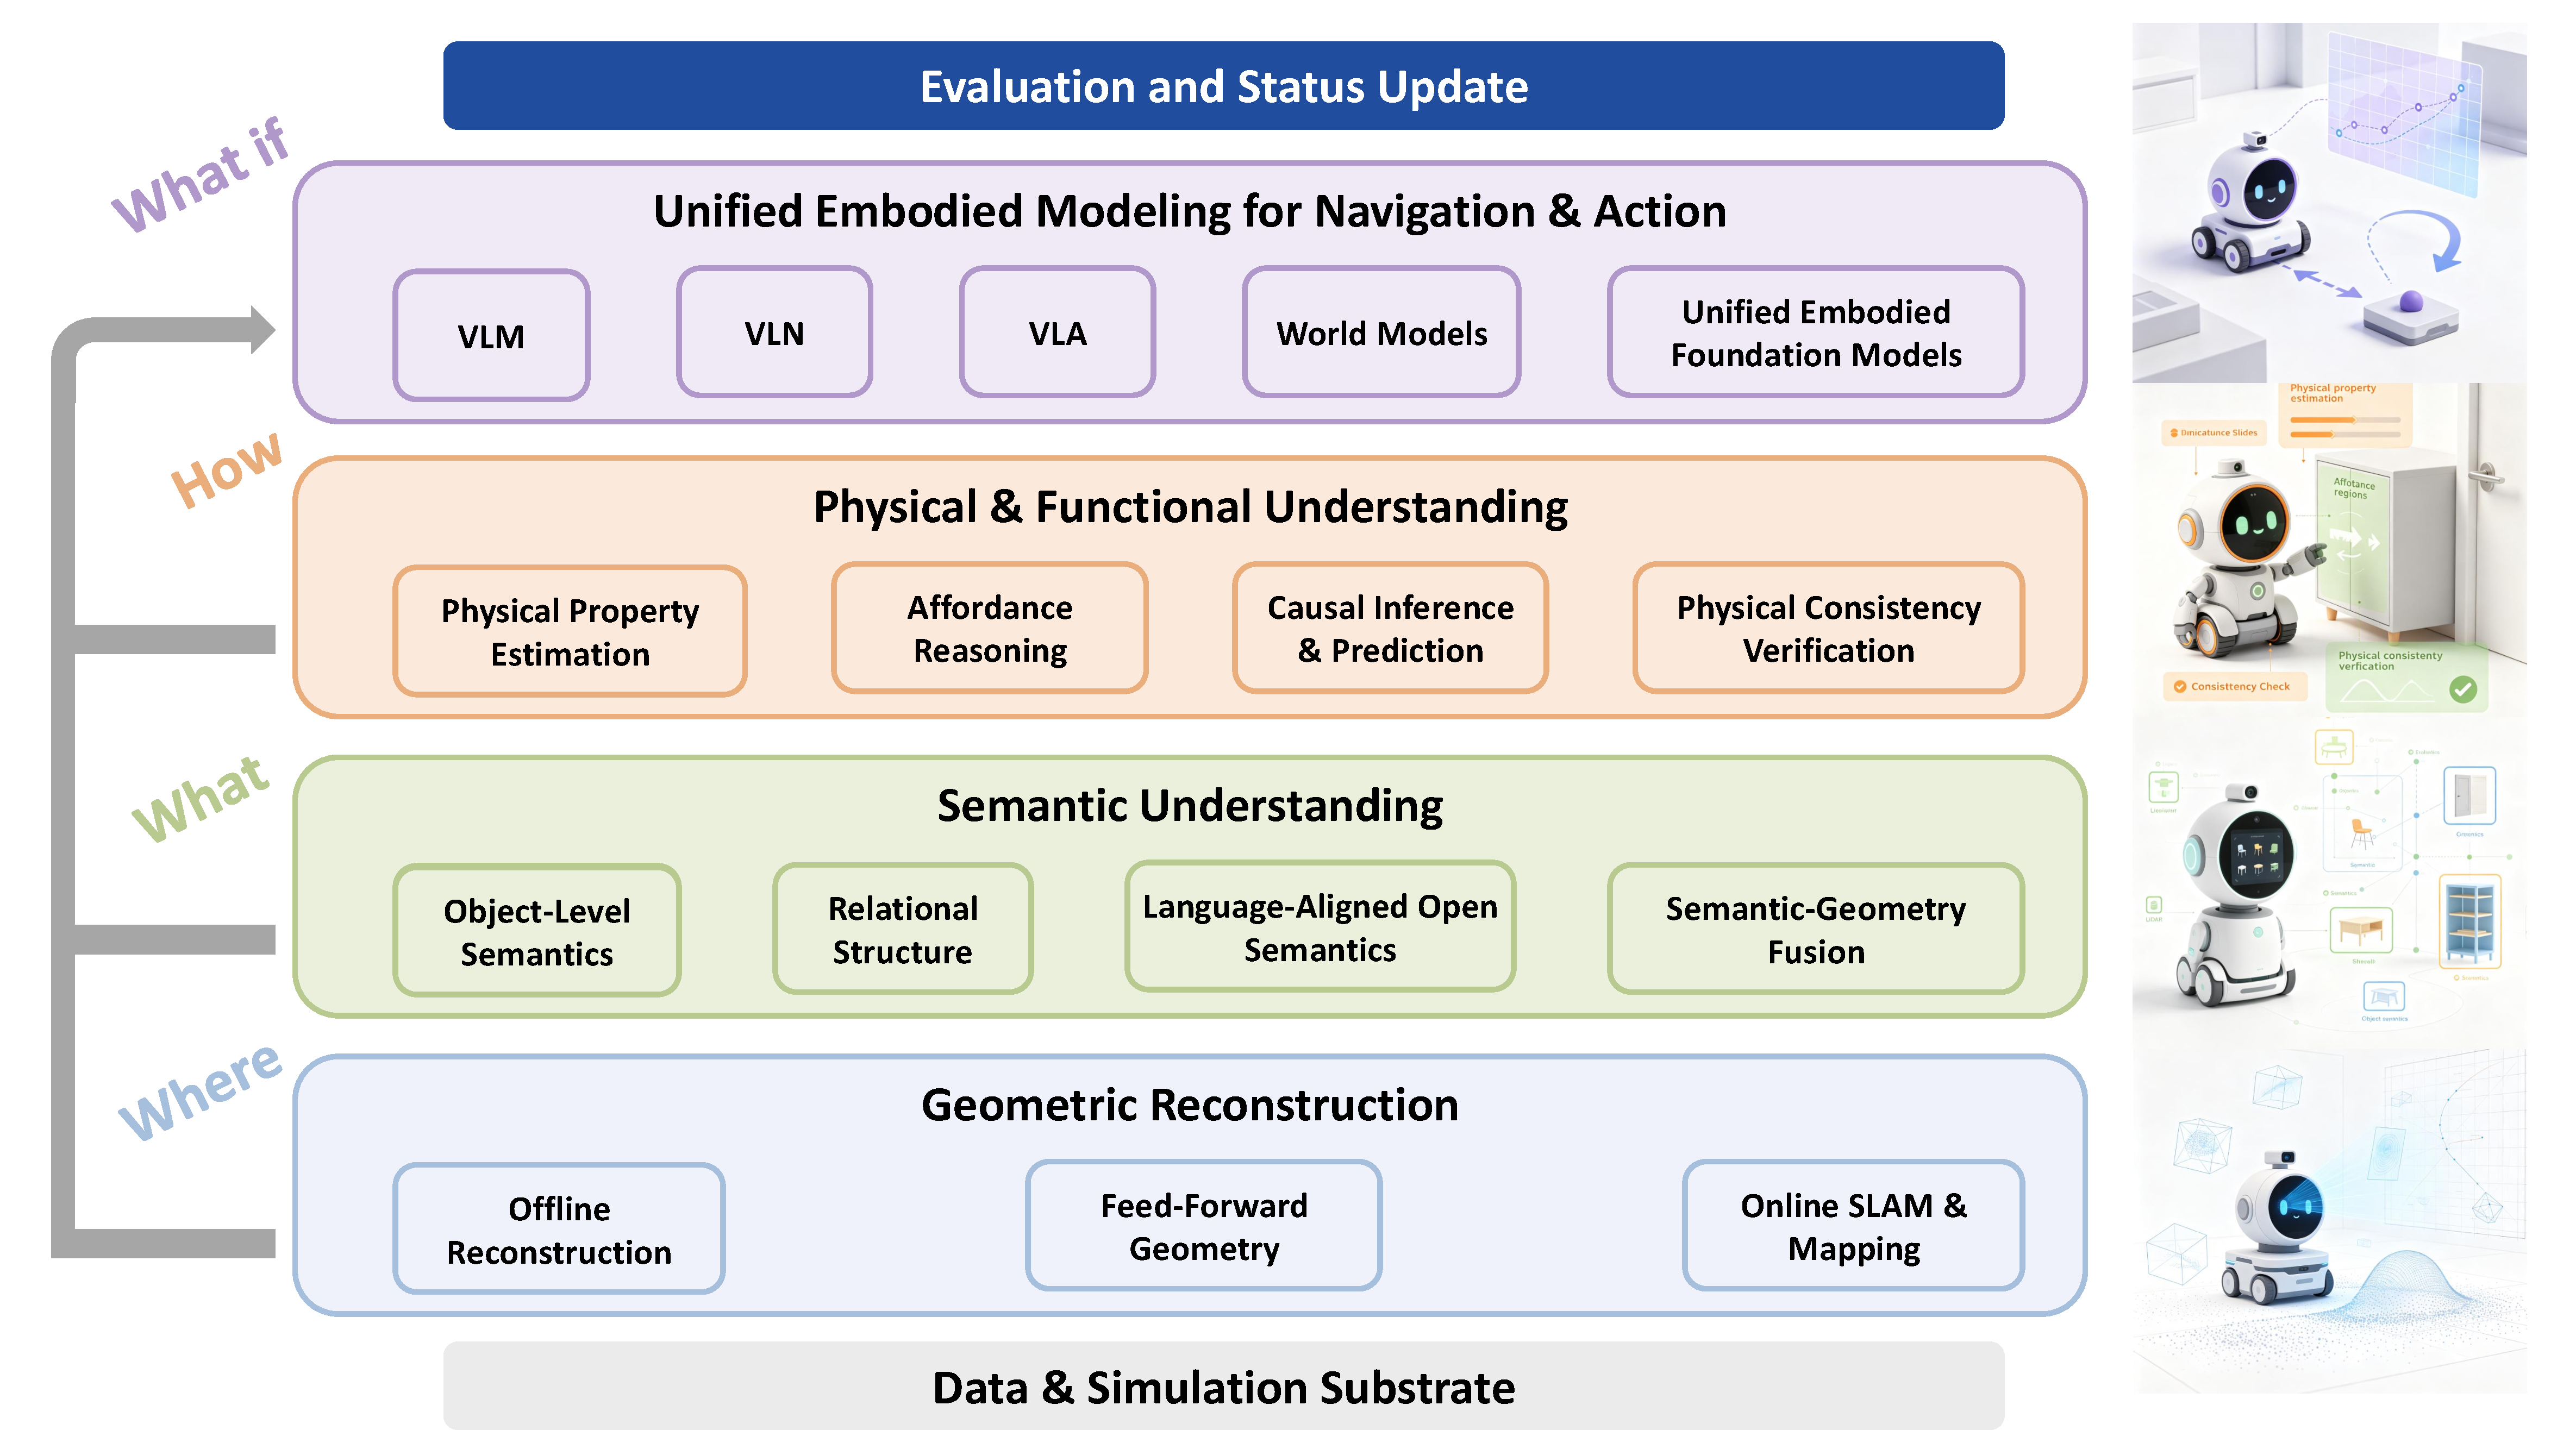
\includegraphics[width=\textwidth]{Figures/fig_framework.pdf}
    \caption{\textbf{A comprehensive view of actionable scene understanding for
    embodied manipulation.} We organize existing research around a shared
    foundation of datasets and simulation environments and four complementary
    aspects of scene understanding: geometric reconstruction establishes spatial
    structure and answers where; semantic understanding identifies objects,
    attributes, and relations and answers what; functional and physical
    understanding characterizes object functions, affordances, and physical
    constraints and addresses how; and task-oriented action connects scene
    understanding to task-relevant navigation and manipulation, addressing where
    to go and what to do. Together, these aspects extend scene understanding from
    describing the environment to supporting task-relevant actions in embodied
    settings.}
    \label{fig:survey_framework}
\end{figure}

\section{Introduction}
\label{sec:introduction}
% Scene understanding provides the perceptual basis for embodied agents to navigate and act in physical environments. For an embodied agent, understanding a scene goes beyond recovering its spatial structure or recognizing the objects it contains. The agent must also determine how objects can be used, which actions they afford, and what physical constraints govern their interaction. These requirements become particularly important when agents operate in complex environments, where task execution depends on both the current scene state and its possible changes following an action. Thus, effective embodied behavior requires scene knowledge that is not only perceptually accurate, but also relevant to task execution.

Scene understanding provides the perceptual basis for embodied agents to navigate and act in physical environments. For manipulation, however, recovering spatial structure and recognizing object categories are only necessary conditions for reliable behavior. An agent must also identify task-relevant entities and regions~\cite{do2018affordancenet,delitzas2024scenefun3d,zhang2025functional3d}, determine which actions are physically feasible~\cite{mo2021where2act,halacheva2025articulate3d}, anticipate how the scene may change under those actions~\cite{bear2021physion,ha2018world,hafner2023mastering}, and update its understanding as new evidence becomes available. Scene understanding for embodied manipulation is therefore not only a problem of describing the current environment, but also of maintaining a representation that supports task-conditioned decision making and physically grounded action.

% In this survey, we use \emph{actionable scene understanding} to denote scene knowledge that enables an embodied agent to reason about, select, and execute actions in a given task context. Unlike conventional scene understanding, which primarily characterizes scene geometry and semantics, actionable scene understanding further incorporates functional, physical, causal, and dynamic knowledge relevant to action. We summarize this distinction as
% \begin{equation}
% \text{Observation}
% \longrightarrow
% \underbrace{\{\mathcal{G},\mathcal{S}\}}_{\text{Conventional Scene Understanding}},
% \end{equation}
% and
% \begin{equation}
% \text{Observation}
% \longrightarrow
% \underbrace{\{\mathcal{G},\mathcal{S},\mathcal{F},\mathcal{P},\mathcal{R},\mathcal{E}\}}_{\text{Actionable Scene Understanding}}
% \longrightarrow
% \mathcal{A},
% \label{eq:actionable_scene_understanding}
% \end{equation}
% where $\mathcal{G}$ denotes geometric structure, $\mathcal{S}$ semantic information, $\mathcal{F}$ functional and affordance information, $\mathcal{P}$ physical properties and constraints, $\mathcal{R}$ causal relations between actions and their effects, $\mathcal{E}$ state evolution under actions, and $\mathcal{A}$ task-oriented actions, with particular emphasis on embodied manipulation. These knowledge dimensions are complementary rather than strictly sequential: geometry and semantics establish what exists and where it is, functional knowledge describes what can be done, physical knowledge constrains what is feasible, causal knowledge relates actions to their effects, and state evolution characterizes how the scene changes over time.
We use \emph{actionable scene understanding} to denote scene knowledge that is sufficiently grounded in the task, spatial configuration, and physical state of an environment to support feasible action selection and execution. Unlike conventional scene understanding, which primarily characterizes geometric structure and semantic content, actionable scene understanding additionally considers functional affordances, physical properties and constraints, causal relations, and state evolution that are relevant to embodied behavior. We summarize this distinction as
\begin{equation}
O \rightarrow \{G,S\},
\end{equation}
\begin{equation}
O_t \rightarrow
\mathcal{S}_t
=
\{G_t,S_t,F_t,P_t,R_t,E_t,U_t\}
\rightarrow
A_t,
\end{equation}
for actionable scene understanding, where $t$ denotes the current time step, $O_t$ denotes the observation, $G_t$ denotes geometric structure, $S_t$ semantic information, $F_t$ functional and affordance information, $P_t$ physical properties and constraints, $R_t$ causal and relational dependencies relevant to action, $E_t$ state evolution, and $A_t$ a task-oriented action.

The key distinction is therefore not the amount of information contained in a scene representation, but its utility for task-conditioned behavior. Given a task context $\mathcal{T}_t$, an embodied agent selects an action according to
\begin{equation}
A_t=\pi(\mathcal{S}_t,\mathcal{T}_t),
\end{equation}
while the executed action may induce a subsequent scene state
\begin{equation}
\mathcal{S}_{t+1}=f(\mathcal{S}_t,A_t),
\end{equation}
where $f$ denotes the physical and environmental transition, and $\pi$ denotes the policy function. Under this formulation, actionability refers to whether the maintained scene state contains the spatial, semantic, functional, physical, and predictive information required to assess action feasibility and anticipate relevant consequences. \emph{Thus, actionability should not be interpreted as richer scene description alone: a representation is actionable only to the extent that its information remains useful under a specific task, physical constraint, and action space.}

These knowledge dimensions should not be interpreted as a strictly sequential processing pipeline. The hierarchy adopted in this survey (Fig.~\ref{fig:survey_framework}) is primarily an organizational abstraction that reflects the increasing functional requirements placed on scene knowledge, whereas an embodied system operates through coupled and recurrent dependencies. Geometry provides spatial grounding for semantic interpretation; semantics determines which entities and regions are relevant to a task; physical and functional knowledge constrains feasible actions; and predicted consequences influence subsequent decisions. Conversely, actions can generate new visual, tactile, or proprioceptive evidence that updates geometry, semantic state, physical estimates, and affordances. \emph{Actionable scene understanding is therefore better viewed as a set of interdependent capabilities embedded within a closed perception--reasoning--action loop, rather than as a strictly hierarchical processing pipeline.}

From this perspective, this survey unifies the transition from perceptual scene reconstruction to actionable scene understanding that is task-relevant, physically grounded, and predictive for embodied manipulation, and highlights both the complementary roles of different knowledge dimensions and the persistent gaps in bridging them.

We further identify four emerging directions toward more capable scene representations: inferring invisible states from visual observations, acquiring physical knowledge through self-supervision, modeling latent human states, and shifting from task completion to human-centered assistance. Collectively, these directions point toward scene understanding that is geometrically and semantically grounded, physically consistent, context-aware, and adaptive to complex real-world environments.

This survey is organized as follows. Section~\ref{sec:data_and_simulation} reviews datasets, simulation environments, and evaluation metrics. Section~\ref{sec:geometric_reconstruction} surveys geometric reconstruction methods, covering offline optimization, feed-forward prediction, and online mapping. Section~\ref{sec:semantic_understanding} reviews semantic understanding, from object-level perception and relational modeling to language-grounded semantics and geometry--semantic unified representations. Section~\ref{sec:physical_functional} focuses on physical and functional understanding relevant to embodied manipulation. Section~\ref{sec:executable_manipulation} discusses executable embodied manipulation, spanning multimodal scene reasoning, spatial and task-level decision making, action generation and control, and predictive modeling, as well as their integration into unified embodied models. Section~\ref{sec:conclusion} summarizes the key advances of the survey and discusses open challenges and future directions, including the modeling of latent human states and emotions for human-aware assistance.

\section{Datasets and Evaluation Metrics}
\label{sec:data_and_simulation}
Datasets and evaluation protocols determine not only which capabilities can be learned, but also which aspects of scene understanding are considered successful. Early indoor scene understanding benchmarks primarily evaluated geometric reconstruction and localization, followed by semantic and instance-level interpretation. More recent datasets incorporate functional parts, articulated structures, interaction affordances, physical properties, temporal states, and task-oriented supervision. This evolution reflects a broader shift from static scene description toward embodied behavior. However, the capability layers are still commonly annotated and evaluated in isolation. To make this structure explicit, Table~\ref{tab:datasets} organizes representative indoor datasets along seven capability dimensions that jointly determine whether a dataset can support actionable scene understanding: \emph{geometry} (meshes, point clouds, or depth-based reconstruction), \emph{semantics} (semantic, instance, or object-level annotations), \emph{physical} (physics simulation or physical-property annotations), \emph{temporal} (sequential or time-series observations), \emph{interaction} (interactive environments or articulated structures), \emph{action} (task suites, demonstrations, or trajectory annotations), and \emph{language} (natural-language grounding or instructions). For each dimension, a dataset is marked as fully, partially, or not supported, and the data source column records how the underlying data were captured or generated, ranging from commodity depth sensors and laser scanning to procedural simulation and volunteer-collected video. Reading across the table exposes the central gap that motivates this survey: perceptual supervision concentrates in the geometry and semantics columns, physical, interaction, and action supervision appears mainly in simulated environments, and language annotations rarely coincide with physically grounded actions. A central question for actionable scene understanding is therefore not only which datasets or metrics are available, but whether their supervision and evaluation preserve the information required for downstream action. In this section, we provide a comprehensive overview of existing datasets and their commonly adopted evaluation protocols, and then discuss emerging evaluation directions and our preliminary reflections on designing metrics that better reflect actionability.
\definecolor{DataGreen}{RGB}{218,233,225}
\definecolor{DataBlue}{RGB}{216,229,241}
\definecolor{DataYellow}{RGB}{247,236,202}
\definecolor{DataRed}{RGB}{243,220,221}

\begin{table}[!tbp]
\centering
\scriptsize
\renewcommand{\arraystretch}{1.0}
\setlength{\tabcolsep}{1.2pt}
\renewcommand{\cmark}{\color{ForestGreen}{\ding{51}}}
\renewcommand{\xmark}{\color{BrickRed}{\ding{55}}}
\newcommand{\limmark}{\textcolor{Orange}{\ding{119}}}

\caption{Representative indoor scene datasets and their supported scene understanding capabilities.}
\label{tab:datasets}
\vspace{1pt}

\resizebox{\textwidth}{!}{
\begin{tabular}{
    >{\centering\arraybackslash}m{2.3cm}   % Dataset
    >{\centering\arraybackslash}m{1.5cm}   % Venue
    >{\centering\arraybackslash}m{1.9cm}   % Scene Type
    >{\centering\arraybackslash}m{1.35cm}  % Geometry
    >{\centering\arraybackslash}m{1.35cm}  % Semantics
    >{\centering\arraybackslash}m{1.35cm}  % Physical
    >{\centering\arraybackslash}m{1.35cm}  % Temporal
    >{\centering\arraybackslash}m{1.35cm}  % Interaction
    >{\centering\arraybackslash}m{1.35cm}  % Action
    >{\centering\arraybackslash}m{1.35cm}  % Language
    >{\centering\arraybackslash}m{2.5cm} % Scene capability
    >{\raggedright\arraybackslash}m{2.4cm}   % Data Source
    >{\raggedright\arraybackslash}m{4.5cm} % Description
}
\toprule
\rowcolor{TableNavy}
\textcolor{white}{Dataset}
& \textcolor{white}{Venue}
& \textcolor{white}{Scene Type}
& \textcolor{white}{Geometry} & \textcolor{white}{Semantics} & \textcolor{white}{Physical} & \textcolor{white}{Temporal} &
\textcolor{white}{Interaction} & \textcolor{white}{Action} & \textcolor{white}{Language}
& \textcolor{white}{\makebox[2.5cm][c]{Scene capability}}
& \textcolor{white}{\makebox[2.4cm][c]{Data Source}}
& \textcolor{white}{\makebox[4.5cm][c]{Description}}
\\
\hline
% ------------------------------------------------------------------------
% Geometric Reconstruction (Sec. III)
% ------------------------------------------------------------------------
\rowcolor{GreenBG}
TUM RGB-D~\cite{sturm2012benchmark}
& IROS'12 & Real-World
& \cmark & \xmark & \xmark & \cmark &
\xmark & \xmark & \xmark
& Geometry
& Microsoft Kinect Camera
& Classic benchmark captured using a Kinect in office and household environments; widely used for RGB-D SLAM evaluation
\\

\rowcolor{GreenBG}
Replica~\cite{straub2019replica}
& arXiv'19 & Synthetic
& \cmark & \cmark & \xmark & \xmark &
\xmark & \xmark & \xmark
& Geometry + Semantics
& RGB-D Capture + Mesh Reconstruction
& Extremely high-fidelity indoor reconstructions for simulation
\\

\rowcolor{GreenBG}
ARKitScenes~\cite{baruch2021arkitscenes}
& NeurIPS'21 & Real-World
& \cmark & \cmark & \xmark & \cmark &
\xmark & \xmark & \xmark
& Geometry
& iPhone/iPad LiDAR + Laser Scanner
& Large-scale real-world indoor dataset captured using Apple LiDAR devices
\\

\rowcolor{GreenBG}
DL3DV-10K~\cite{ling2024dl3dv}
& CVPR'24 & Real-World
& \cmark & \xmark & \xmark & \cmark &
\xmark & \xmark & \xmark
& Geometry
& Volunteer Mobile/Drone Videos
& 51.2M frames from 10,510 real-world videos across 65 POI types (indoor and bounded scenes) for feed-forward 3D reconstruction
\\

\rowcolor{GreenBG}
ScanNet++~\cite{yeshwanth2023scannet++}
& ICCV'23 & Real-World
& \cmark & \cmark & \xmark & \cmark &
\xmark & \xmark & \xmark
& Geometry + Semantics
& High-end Laser Scanner + DSLR + iPhone RGB-D
& Successor to ScanNet with significantly higher geometric and photometric fidelity
\\

\rowcolor{GreenBG}
HiRoom~\cite{lin2025depthanything3}
& arXiv'25 & Synthetic
& \cmark & \xmark & \xmark & \limmark &
\xmark & \xmark & \xmark
& Geometry
& Blender Rendering
& Professional-artist Blender-rendered indoor living scenes for camera-pose, depth, and geometry benchmarking (Depth Anything 3)
\\

\rowcolor{GreenBG}
Holo360D~\cite{ou2026holo360d}
& arXiv'26 & Real-World
& \cmark & \xmark & \xmark & \cmark &
\xmark & \xmark & \xmark
& Geometry
& 3D Laser Scanner + 360 Camera + SLAM
& 109,495 real-world panoramas with continuous trajectories, registered point clouds, meshes, and aligned camera poses
\\

\hline
% ------------------------------------------------------------------------
% Semantic Understanding (Sec. IV)
% ------------------------------------------------------------------------
\rowcolor{BlueBG}
NYU Depth V2~\cite{silberman2012indoor}
& ECCV'12 & Real-World
& \cmark & \cmark & \xmark & \cmark &
\xmark & \xmark & \xmark
& Geometry + Semantics
& Microsoft Kinect Camera
& Landmark indoor RGB-D benchmark with 1449 densely labeled scenes
\\

\rowcolor{BlueBG}
S3DIS~\cite{armeni20163d}
& CVPR'16 & Real-World
& \cmark & \cmark & \xmark & \xmark &
\xmark & \xmark & \xmark
& Geometry + Semantics
& Matterport Scanner
& Extension of the Stanford indoor semantic dataset with larger-scale annotations
\\

\rowcolor{BlueBG}
ScanNet~\cite{dai2017scannet}
& CVPR'17 & Real-World
& \cmark & \cmark & \xmark & \cmark &
\xmark & \xmark & \xmark
& Geometry + Semantics
& iPad + Structure Sensor RGB-D
& One of the most influential RGB-D indoor reconstruction datasets; 2.5M views across 1513 scenes
\\

\rowcolor{BlueBG}
Structured3D~\cite{zheng2020structured3d}
& ECCV'20 & Synthetic
& \cmark & \cmark & \xmark & \xmark &
\xmark & \xmark & \xmark
& Geometry + Semantics
& Procedural Layouts + Rendering
& Large-scale synthetic structured indoor scenes with layout annotations
\\

\rowcolor{BlueBG}
Infinigen Indoors~\cite{raistrick2024infinigen}
& CVPR'24 & Synthetic
& \cmark & \cmark & \cmark & \limmark &
\limmark & \xmark & \xmark
& Geometry + Semantics
& Procedural Generation (Blender)
& Photorealistic procedurally generated indoor scenes with ground-truth depth, segmentation, and meshes
\\

\rowcolor{BlueBG}
ToF-360~\cite{kanayama2025tof360}
& CVPRW'25 & Real-World
& \cmark & \cmark & \xmark & \xmark &
\xmark & \xmark & \xmark
& Geometry + Semantics
& 360-degree ToF Sensor (Single Capture)
& First panoramic ToF RGB-D dataset enabling single-capture 360-degree indoor scanning with high-quality semantic and room-layout annotations
\\

\rowcolor{BlueBG}
XScene~\cite{li2026scenix}
& arXiv'26 & Hybrid
& \cmark & \limmark & \xmark & \xmark &
\xmark & \xmark & \limmark
& Geometry + Semantics
& Synthetic Rendering + Real Capture
& $\sim$110K synthetic and real indoor scenes with room structures, object descriptions, and metric spatial annotations for sparse-view reconstruction
\\

\hline
% ------------------------------------------------------------------------
% Physical and Functional Understanding (Sec. V)
% ------------------------------------------------------------------------
\rowcolor{OrangeBG}
AI2-THOR~\cite{kolve2017ai2}
& arXiv'17 & Synthetic
& \cmark & \cmark & \cmark & \xmark &
\cmark & \limmark & \xmark
& Physical/Interactive
& Procedural Modeling + Physics Engine
& Interactive household scenes with actionable objects and physics-based interactions
\\

\rowcolor{OrangeBG}
SAPIEN~\cite{xiang2020sapien}
& CVPR'20 & Synthetic
& \cmark & \cmark & \cmark & \xmark &
\cmark & \limmark & \xmark
& Physical/Interactive
& PartNet-Mobility Articulated CAD
& Realistic physics simulation with articulated objects for interaction and manipulation
\\

\rowcolor{OrangeBG}
OpenRooms~\cite{li2021openrooms}
& CVPR'21 & Synthetic
& \cmark & \cmark & \limmark & \xmark &
\xmark & \xmark & \xmark
& Geometry
& Physically-based Rendering
& Large-scale photorealistic indoor rendering benchmark with geometry and material labels
\\

\rowcolor{OrangeBG}
ReplicaCAD~\cite{szot2021habitat}
& NeurIPS'21 & Synthetic
& \cmark & \cmark & \cmark & \xmark &
\cmark & \limmark & \xmark
& Physical/Interactive
& CAD Modeling + Articulation
& High-fidelity articulated household scenes for rearrangement and interaction
\\

\rowcolor{OrangeBG}
ProcTHOR~\cite{deitke2022}
& NeurIPS'22 & Synthetic
& \cmark & \cmark & \cmark & \xmark &
\cmark & \limmark & \xmark
& Physical/Interactive
& Procedural Generation
& Thousands of procedurally generated interactive houses for scalable embodied learning
\\

\rowcolor{OrangeBG}
BEHAVIOR-1K~\cite{li2023behavior}
& CoRL'23 & Synthetic
& \cmark & \cmark & \cmark & \xmark &
\cmark & \cmark & \limmark
& Physical/Interactive
& OmniGibson Sim + wikiHow Activities
& 1,000 everyday activities in realistic interactive households for long-horizon task evaluation
\\

\rowcolor{OrangeBG}
ManiSkill3~\cite{tao2025maniskill3}
& RSS'25 & Synthetic
& \cmark & \limmark & \cmark & \cmark &
\cmark & \cmark & \limmark
& Physical/Interactive
& GPU-Parallel Physics Simulation
& GPU-parallel contact-rich manipulation simulation and rendering across 12 task domains
\\

\hline
% ------------------------------------------------------------------------
% Embodied Navigation and Manipulation (Sec. VI)
% ------------------------------------------------------------------------
\rowcolor{PurpleBG}
Matterport3D~\cite{chang2017matterport3d}
& CVPR'17 & Real-World
& \cmark & \limmark & \xmark & \xmark &
\xmark & \xmark & \xmark
& Navigation
& Matterport Camera System
& Building-scale RGB-D dataset with globally aligned panoramic scans
\\

\rowcolor{PurpleBG}
Gibson~\cite{xia2018gibson}
& CVPR'18 & Real-World
& \cmark & \xmark & \xmark & \limmark &
\limmark & \xmark & \xmark
& Navigation
& Matterport Real Scans + Rendering
& Photorealistic real-world spaces for embodied navigation
\\

\rowcolor{PurpleBG}
HM3D~\cite{ramakrishnan2021habitat}
& arXiv'21 & Real-World
& \cmark & \xmark & \xmark & \xmark &
\xmark & \xmark & \xmark
& Navigation
& Matterport Scanning
& 1000 large-scale building reconstructions for embodied AI training
\\

\rowcolor{PurpleBG}
HM3D-Sem~\cite{yadav2023habitat}
& CVPR'23 & Real-World
& \cmark & \cmark & \xmark & \xmark &
\xmark & \xmark & \xmark
& Navigation
& Matterport Scans (HM3D)
& Semantic extension of HM3D with 142k+ object instances
\\

\rowcolor{PurpleBG}
ManiSkill2~\cite{gu2023maniskill2}
& arXiv'23 & Synthetic
& \cmark & \limmark & \cmark & \cmark &
\cmark & \cmark & \xmark
& Manipulation
& Physics Simulation + Task Suite
& Contact-rich manipulation benchmark with accurate dynamics
\\

\rowcolor{PurpleBG}
HSSD-200~\cite{khanna2024hssd}
& CVPR'24 & Synthetic
& \cmark & \cmark & \limmark & \xmark &
\limmark & \limmark & \xmark
& Navigation
& Designer Modeling + Curation
& 211 high-quality synthetic houses with 18.6K real-object models across 466 semantic categories
\\

\rowcolor{PurpleBG}
RoboCasa~\cite{nasiriany2024robocasa}
& arXiv'24 & Hybrid
& \cmark & \limmark & \cmark & \cmark &
\cmark & \cmark & \cmark
& Manipulation
& Procedural + Real Kitchens
& Large-scale kitchen manipulation with parallel simulated and real evaluation suites
\\

\rowcolor{PurpleBG}
InternScenes~\cite{zhong2025internscenes}
& arXiv'25 & Hybrid
& \cmark & \cmark & \cmark & \xmark &
\limmark & \limmark & \xmark
& Physical/Interactive
& Real-to-Sim + Procedural Generation
& ~40K simulatable indoor scenes with 1.96M objects, 800K CAD models across 288 classes and realistic cluttered layouts
\\

\hline
% ------------------------------------------------------------------------
% Generalist Embodied and Multimodal Foundation (Sec. VI)
% ------------------------------------------------------------------------
\rowcolor{CyanBG}
EmbodiedScan~\cite{wang2024embodiedscan}
& CVPR'24 & Real-World
& \cmark & \cmark & \xmark & \cmark &
\xmark & \xmark & \cmark
& Generalist Embodied
& Aggregated Real Scans (ScanNet + 3RScan + MP3D)
& Unified multi-modal benchmark for embodied 3D understanding with language grounding
\\

\rowcolor{CyanBG}
GRUtopia~\cite{wang2024grutopia}
& arXiv'24 & Synthetic
& \cmark & \cmark & \cmark & \limmark &
\cmark & \cmark & \cmark
& Generalist Embodied
& Designer-Sourced Synthetic Scenes
& 100K interactive scenes for city-scale embodied service robots with LLM-driven NPCs
\\

\rowcolor{CyanBG}
MolmoBot-Data~\cite{deshpande2026molmobot}
& arXiv'26 & Synthetic
& \cmark & \limmark & \cmark & \cmark &
\cmark & \cmark & \cmark
& Generalist Embodied
& Simulated Trajectory Generation
& 1.8M simulated trajectories enabling zero-shot sim-to-real transfer
\\

\rowcolor{CyanBG}
RoboDojo~\cite{chen2026robodojo}
& arXiv'26 & Hybrid
& \cmark & \cmark & \cmark & \cmark &
\cmark & \cmark & \cmark
& Generalist Embodied
& Unified Task Suite (Sim + Real)
& 42 simulated and 18 real-world manipulation tasks for generalist policy evaluation
\\

\rowcolor{CyanBG}
SceneVerse++~\cite{chen2026lifting}
& CVPR'26 & Web-Scale
& \cmark & \cmark & \xmark & \xmark &
\xmark & \xmark & \cmark
& Generalist Embodied
& Multi-source Real Scans + Synthetic Scenes
& Large-scale indoor 3D scenes reconstructed from internet videos
\\

\rowcolor{CyanBG}
SIMPLE~\cite{wei2026simple}
& arXiv'26 & Synthetic
& \cmark & \xmark & \cmark & \cmark &
\cmark & \cmark & \cmark
& Generalist Embodied
& Whole-Body Simulation
& Whole-body humanoid loco-manipulation benchmark
\\
\hline

\end{tabular}}
\vspace{2pt}

{\scriptsize Note. \cmark{} fully supported \quad \xmark{} not supported \quad \limmark{} partially supported}
\vspace{2pt}
\end{table}
\subsection{Geometric and Semantic Scene Understanding}
\label{subsec:geometric_semantic_datasets} Early indoor datasets established the geometric basis for scene reconstruction, localization, and spatial perception. TUM RGB-D, ICL-NUIM, and 7-Scenes provide RGB-D observations, camera trajectories, or accurate pose and geometric annotations, and have served as standard benchmarks for visual tracking and reconstruction ~\cite{sturm2012benchmark,handa2014benchmark,shotton2013scene}. Large-scale datasets such as SUN RGB-D, S3DIS, ScanNet, and Matterport3D subsequently introduced object- and scene-level semantic annotations, enabling joint geometric and semantic understanding ~\cite{song2015sunrgbd,armeni20163d,dai2017scannet,chang2017matterport3d}. More recent datasets have emphasized higher geometric fidelity, multimodal observations, and richer scene variation ~\cite{straub2019replica,ling2024dl3dv}. ARKitScenes provides large-scale indoor scans acquired with commodity sensing devices, while ScanNet++ combines high-quality 3D scanning with high-resolution visual observations
~\cite{baruch2021arkitscenes,yeshwanth2023scannet++}. 3RScan further introduces repeated scans of the same environments, enabling the study of scene changes and object reconfigurations ~\cite{wald2019rio}. EmbodiedScan extends large-scale 3D perception toward
egocentric embodied settings by organizing RGB-D observations and annotations around continuous first-person scene exploration
~\cite{wang2024embodiedscan}. Despite their increasing scale and annotation richness, these datasets remain largely descriptive. They characterize scene geometry, object identity, and spatial relationships, but generally provide limited supervision for object
function, physical state, or action consequences. Thus, they establish the perceptual foundation for actionable scene understanding rather than directly solving it. In Table~\ref{tab:datasets}, this group occupies the geometry and semantics columns almost exclusively: every dataset in this group fully supports geometric supervision, most provide semantic or instance annotations, and none provides physical, interaction, or action supervision.
\begin{table}[!t]
    \centering
    \caption{\textbf{Evaluation metrics for actionable indoor scene understanding.} Metrics are organized along the four capability layers of this survey, covering rendering and geometric quality, semantic and relational accuracy, physical plausibility, and task-level success.}
    \label{tab:evaluation_metrics}
    \vspace{0.15em}
    \scriptsize
    \setlength{\tabcolsep}{1.2pt}
    \renewcommand{\arraystretch}{1.0}
    \resizebox{\textwidth}{!}{%
    \begin{tabular}{@{} >{\RaggedRight\arraybackslash}m{2.4cm} >{\RaggedRight\arraybackslash}m{4.6cm} >{\RaggedRight\arraybackslash}m{8.2cm} >{\RaggedRight\arraybackslash}m{3.2cm} @{}}
        \toprule
        \rowcolor{TableNavy}
        \color{white}\bfseries\Centering Sub-dimension & \color{white}\bfseries\Centering Metric / direction & \color{white}\bfseries\Centering What it measures & \color{white}\bfseries\Centering Classic Method \\
        \arrayrulecolor{TableNavy}
        \midrule

        \rowcolor{TableSub}
        \multicolumn{4}{@{}l}{\hspace{0.12em}\textcolor{TableNavy}{\bfseries I.\;Geometric reconstruction}}\\[0.6em]
        \arrayrulecolor{GrayRule}

        SfM & Reprojection Error $\downarrow$; Camera Pose Error $\downarrow$ & Projection-to-feature image distance; accuracy of estimated camera parameters. & Bundler, COLMAP \\

        \cmidrule[0.25pt](lr){1-4}
        MVS & Accuracy / Completeness / Overall $\downarrow$; F-Score $\uparrow$ & Surface accuracy vs. reference coverage; precision--recall balance. & PatchMatch Stereo, MVSNet \\

        \cmidrule[0.25pt](lr){1-4}
        NeRF & PSNR $\uparrow$; SSIM $\uparrow$; LPIPS $\downarrow$; Chamfer Distance $\downarrow$ & Pixel, structural, and perceptual rendering fidelity; extracted-surface quality. & NeRF, NeuS, Instant-NGP \\

        \cmidrule[0.25pt](lr){1-4}
        3DGS & PSNR $\uparrow$; SSIM $\uparrow$; LPIPS $\downarrow$; Chamfer Distance $\downarrow$ & Novel-view rendering fidelity; geometric accuracy of surfaces extracted from Gaussians. & 3DGS, SuGaR, 2DGS \\

        \cmidrule[0.25pt](lr){1-4}
        Pointmap-based 3D foundation models & CD $\downarrow$; F-Score $\uparrow$; Camera Pose Error $\downarrow$ & Pointmaps and camera parameters predicted from one or a few images. & DUSt3R, MASt3R, VGGT \\

        \cmidrule[0.25pt](lr){1-4}
        Classical, neural, and Gaussian SLAM & ATE RMSE $\downarrow$; RPE $\downarrow$; PSNR $\uparrow$; CD $\downarrow$ & Trajectory error and local drift; rendering and geometry quality of online maps. & ORB-SLAM, NICE-SLAM, MonoGS \\

        \cmidrule[0.25pt](lr){1-4}
        Dynamic and action-induced reconstruction & Dynamic Object Tracking Error $\downarrow$; Update Latency $\downarrow$; Temporal Consistency $\downarrow$ & Dynamic object tracking, scene-update latency, and temporal consistency. & DynamicFusion, deformable Gaussians, D4RT \\

        \cmidrule[0.25pt](lr){1-4}
        Multi-agent reconstruction & Global Consistency Error $\downarrow$; Communication Overhead $\downarrow$; ATE RMSE $\downarrow$ & Global consistency of fused maps; communication efficiency; per-agent trajectory accuracy. & COVINS, Swarm-SLAM \\

        \arrayrulecolor{TableNavy}
        \cmidrule[0.50pt]{1-4}

        \rowcolor{TableSub}
        \multicolumn{4}{@{}l}{\hspace{0.12em}\textcolor{TableNavy}{\bfseries II.\;Semantic understanding}}\\[0.6em]
        \arrayrulecolor{GrayRule}

        Semantic segmentation & mIoU $\uparrow$; Overall / Mean Accuracy $\uparrow$ & Mean per-class IoU and point-wise classification accuracy. & ScanNet, S3DIS; PointNet++ \\

        \cmidrule[0.25pt](lr){1-4}
        Instance and panoptic segmentation & PQ $\uparrow$; AP / mAP $\uparrow$ & Panoptic quality from recognition and segmentation quality; instance average precision. & Mask3D, SoftGroup, OneFormer3D \\

        \cmidrule[0.25pt](lr){1-4}
        3D object detection & mAP $\uparrow$ (IoU@0.25/0.5); NDS $\uparrow$ & Average precision over IoU thresholds for box localization and classification. & VoteNet, FCAF3D, TR3D \\

        \cmidrule[0.25pt](lr){1-4}
        Scene graph generation & Recall@K $\uparrow$ (SGGen / SGCls / PredCls) & Triplet (subject--relation--object) retrieval under the three standard settings. & SGFormer, SDSGG, SceneLLM \\

        \cmidrule[0.25pt](lr){1-4}
        Room layout estimation & Corner Error $\downarrow$; 3D IoU $\uparrow$; Normal Error $\downarrow$ & Layout-corner localization; 2D/3D overlap with the reference layout; wall orientation. & HorizonNet, LED2-Net, uLayout \\

        \cmidrule[0.25pt](lr){1-4}
        3D visual grounding & Accuracy $\uparrow$ (IoU@0.25/0.5); Recall@1 $\uparrow$ & Localization of language-described objects at standard IoU thresholds. & ScanRefer, ReferIt3D, 3D-VisTA \\

        \cmidrule[0.25pt](lr){1-4}
        Open-vocabulary 3D understanding & Zero-shot mIoU $\uparrow$; CLIP Score $\uparrow$ & Zero-shot generalization to unseen categories; 3D--text alignment. & OpenScene, ConceptFusion \\

        \cmidrule[0.25pt](lr){1-4}
        Semantic occupancy & mIoU $\uparrow$; IoU $\uparrow$; F-Score $\uparrow$ & Occupancy geometry, semantic labels, and completion of unobserved regions. & SSCNet, ScanComplete \\

        \arrayrulecolor{TableNavy}
        \cmidrule[0.50pt]{1-4}

        \rowcolor{TableSub}
        \multicolumn{4}{@{}l}{\hspace{0.12em}\textcolor{TableNavy}{\bfseries III.\;Physical and functional understanding}}\\[0.6em]
        \arrayrulecolor{GrayRule}

        Property estimation & MAE / RMSE $\downarrow$; Physical Consistency $\uparrow$ & Numerical accuracy of material and mechanical attributes; physical consistency. & Physion, PhysBench \\

        \cmidrule[0.25pt](lr){1-4}
        Simulation-ready assets & URDF Validity $\uparrow$; Simulation / Task Success $\uparrow$ & Physics-engine import; validity of joints and parameters; downstream task success. & PhysX-3D, PhysX-Anything \\

        \cmidrule[0.25pt](lr){1-4}
        Affordance reasoning & mIoU $\uparrow$; Feasibility Accuracy $\uparrow$; Task Success Rate $\uparrow$ & Interactive-region segmentation; action feasibility under task and physics. & AffordanceNet, Where2Act, RAIL \\

        \cmidrule[0.25pt](lr){1-4}
        Consequence prediction & State Prediction Error $\downarrow$; Violation Rate $\downarrow$ & Post-action pose and velocity prediction; temporal and physical consistency. & CLEVRER, CausalVQA \\

        \cmidrule[0.25pt](lr){1-4}
        Consistency verification & Violation Detection Accuracy $\uparrow$; FVD $\downarrow$ & Detection of physical-law violations; plausibility of generated content. & PhyGenBench \\

        \arrayrulecolor{TableNavy}
        \cmidrule[0.50pt]{1-4}

        \rowcolor{TableSub}
        \multicolumn{4}{@{}l}{\hspace{0.12em}\textcolor{TableNavy}{\bfseries IV.\;Executable embodied manipulation}}\\[0.6em]
        \arrayrulecolor{GrayRule}

        VLMs & VQA Accuracy $\uparrow$; Grounding Accuracy $\uparrow$ & Visual question answering and grounding accuracy. & CLIP, BLIP-2, LLaVA \\

        \cmidrule[0.25pt](lr){1-4}
        Vision-language navigation & Success Rate $\uparrow$ (SR); SPL $\uparrow$; NE $\downarrow$ & Goal-reaching success; path-length-weighted success; goal distance. & R2R, PREVALENT, HAMT, NavGPT \\

        \cmidrule[0.25pt](lr){1-4}
        VLA policies & Task Success Rate $\uparrow$; Action Error $\downarrow$; Grasp Success Rate $\uparrow$ & End-to-end task success; action prediction error; grasp and placement accuracy. & RT-1, RT-2, OpenVLA \\

        \cmidrule[0.25pt](lr){1-4}
        World and action models & Future Prediction Loss $\downarrow$; FVD $\downarrow$; Planning Success Rate $\uparrow$ & Future-state prediction; generated-video fidelity; planning success. & DreamerV3, Genie, GAIA-1 \\

        \cmidrule[0.25pt](lr){1-4}
        Unified embodied modeling & Multi-task Success Rate $\uparrow$; Cross-domain Generalization $\uparrow$ & Multi-task average success and generalization across tasks, scenes, and embodiments. & 3D-VLA, Cosmos \\

        \arrayrulecolor{TableNavy}
        \bottomrule
        \end{tabular}}
    \arrayrulecolor{black}
    \par\vspace{2pt}
    {\raggedright\scriptsize\textit{Note.} Arrows indicate preferred directions. Protocols should specify alignment, thresholds, and task-specific success criteria.\par}
\end{table}
\subsection{Functional and Physical Scene Understanding}
\label{subsec:functional_physical_datasets}
As embodied applications require scene understanding beyond object identity and spatial layout, recent datasets have begun to provide functional, affordance, and physical information. SceneFun3D introduces fine-grained annotations for functional elements in 3D scenes, together with task descriptions, interaction locations, and object motion parameters ~\cite{delitzas2024scenefun3d}. These annotations support functionality segmentation, task-driven affordance grounding, and 3D motion estimation, providing scene information that is directly relevant to manipulation. Articulate3D further extends 3D scene description to articulated objects by
annotating object parts, connectivity, movable components, and motion attributes ~\cite{halacheva2025articulate3d}. Such annotations enable the representation of structural and motion-related properties that are not captured by conventional semantic labels. Functional 3D scene graph benchmarks further model functional relationships between objects and interaction-relevant scene elements, providing structured representations for functional reasoning and robotic applications ~\cite{zhang2025functional3d}. These datasets progressively enrich scene annotations from object categories and spatial relations to functional roles, articulation, affordances, and physical configurations. Compared with conventional semantic datasets, they provide more explicit information about how scene elements participate in potential actions and how their states are related to physical interaction. In Table~\ref{tab:datasets}, physical supervision of this kind remains scarce and is provided mostly by simulation-based datasets such as AI2-THOR, SAPIEN, ReplicaCAD, and BEHAVIOR-1K, which mark the physical column as fully supported, whereas most real-world datasets leave it unsupported.

\subsection{Interactive and Embodied Environments}
\label{subsec:interactive_embodied_datasets}
While real-world datasets provide observations of existing scenes, embodied agents also require environments in which scene states can be modified through actions. Interactive simulation platforms provide controllable scenes, object states, and interaction interfaces for this purpose~\cite{gan2021threedworld,li2020igibson}. AI2-THOR provides interactive indoor environments with object states and executable actions, and SAPIEN provides physically simulated environments with articulated objects for embodied interaction and manipulation
~\cite{kolve2017ai2,xiang2020sapien}. Habitat provides scalable 3D environments for embodied navigation and interaction, supporting large-scale training and evaluation of embodied agents ~\cite{savva2019habitat,szot2021habitat}. More recent environments focus increasingly on manipulation and long-horizon activities. BEHAVIOR-1K introduces a large collection of everyday activities
in simulated household environments, covering diverse objects, scenes, and long-horizon tasks ~\cite{li2023behavior}. RoboCasa provides a scalable simulation framework for learning generalizable robot manipulation skills across diverse household environments ~\cite{nasiriany2024robocasa}. ManiSkill2 provides a large-scale benchmark and simulation framework for manipulation, with diverse objects, tasks, and physically simulated interactions ~\cite{gu2023maniskill2}. Unlike static scene datasets, these environments associate observations with executable actions and resulting state transitions:
\begin{equation}
s_t \xrightarrow{a_t} s_{t+1},
\label{eq:state_transition}
\end{equation}
where $s_t$ denotes the scene state and $a_t$ denotes the executed action. This formulation enables the generation of interaction trajectories and action-conditioned scene states at a scale that is difficult to obtain from real-world data collection.

The development of these datasets reflects a gradual expansion of indoor scene information, from geometric structure and semantic identity to functional properties, physical configurations, and executable interactions. This progression provides increasingly rich data for studying the transition from conventional scene reconstruction and understanding to actionable scene understanding for embodied agents. In Table~\ref{tab:datasets}, these environments are precisely the ones that fill the interaction and action columns left unsupported by perception-oriented datasets, although their language supervision remains limited.

\subsection{Evaluation Metrics}
\label{subsec:evaluation_metrics}
Datasets define the observations and supervision available for learning, while evaluation metrics define how progress toward actionable scene understanding is measured. Table~\ref{tab:evaluation_metrics} summarizes representative evaluation metrics for the tasks reviewed in this survey, organized along the four capability layers: geometric reconstruction, semantic understanding, physical and functional understanding, and embodied manipulation. Rendering metrics such as PSNR, SSIM~\cite{wang2004image}, and LPIPS~\cite{zhang2018perceptual}, together with geometric metrics such as Accuracy, Completeness, Chamfer Distance, F-Score, ATE, and RPE~\cite{sturm2012benchmark}, assess visual fidelity and reconstruction quality; semantic metrics such as mIoU, PQ~\cite{kirillov2019panoptic}, mAP, and Recall@K evaluate recognition, relational, and grounding accuracy; physical and functional metrics measure property estimation, interaction feasibility, and physical plausibility; and embodied metrics such as task success rate, SPL, and planning success quantify task completion and generalization.

\begin{table}[!t]
\centering
\caption{From perceptual evaluation toward actionability-oriented evaluation. The rightmost column represents emerging or desirable evaluation directions rather than universally established standards.}
\label{tab:actionability_evaluation}
\footnotesize
\setlength{\tabcolsep}{5pt}
\renewcommand{\arraystretch}{1.35}
\begin{tabularx}{\textwidth}{>{\RaggedRight\arraybackslash}p{2.3cm} >{\RaggedRight\arraybackslash}X >{\RaggedRight\arraybackslash}X >{\RaggedRight\arraybackslash}X}
\toprule
\rowcolor{TableNavy}
\textcolor{white}{\bfseries Capability}
& \textcolor{white}{\bfseries Existing evaluation}
& \textcolor{white}{\bfseries Action-relevant question}
& \textcolor{white}{\bfseries Actionability-oriented evaluation} \\
\midrule
\rowcolor{TableSub}
Geometry & CD, F-score, Accuracy, Completeness &
Is the relevant geometry correct? &
Contact/collision-aware geometric evaluation \\
Semantics & mIoU, PQ, mAP, Recall@K &
Is the correct entity or part grounded? &
Task-grounded semantic accuracy \\
\rowcolor{TableSub}
Function & Affordance accuracy &
Is the intended interaction feasible? &
Action feasibility and affordance success \\
Physics & Property estimation error &
Are relevant physical constraints captured? &
Physical violation and behavior consistency \\
\rowcolor{TableSub}
Planning & Planning success &
Does the predicted state support decisions? &
Prediction-aware planning performance \\
Embodied Behavior & Task success, SPL &
Does the full system complete the task? &
Closed-loop task success and robustness \\
\bottomrule
\end{tabularx}
\end{table}
\subsection{Actionability Evaluation}
Existing evaluation protocols primarily measure whether a predicted representation agrees with a reference representation. Such measurements are indispensable for assessing individual capabilities, but they do not directly establish whether the representation is useful for embodied action. A low Chamfer distance, for example, does not guarantee accurate contact geometry; high semantic IoU does not guarantee correct identification of the actionable part of an object; and accurate short-term state prediction does not necessarily imply improved planning. These observations motivate a distinction between \emph{perceptual fidelity} and \emph{actionability}.

For a task $\mathcal{T}$, an actionable evaluation should ideally measure whether the predicted scene state preserves the information necessary for a feasible action and whether errors in that state affect the resulting behavior. This suggests a capability chain
\begin{equation}
\begin{split}
\text{Representation} & \rightarrow \text{Task-Relevant Prediction} \\
& \rightarrow \text{Action Feasibility} \\
& \rightarrow \text{Executable Action}.
\end{split}
\end{equation}
Under this view, geometric, semantic, physical, and predictive metrics should be complemented by task-conditioned evaluations rather than treated as interchangeable indicators of scene understanding quality. Therefore, we expect the evaluation metrics summarized in Table~\ref{tab:actionability_evaluation} to guide future actionability-oriented assessment.

\section{Geometric Reconstruction}
\label{sec:geometric_reconstruction}
\begin{figure}[t]
    \centering
    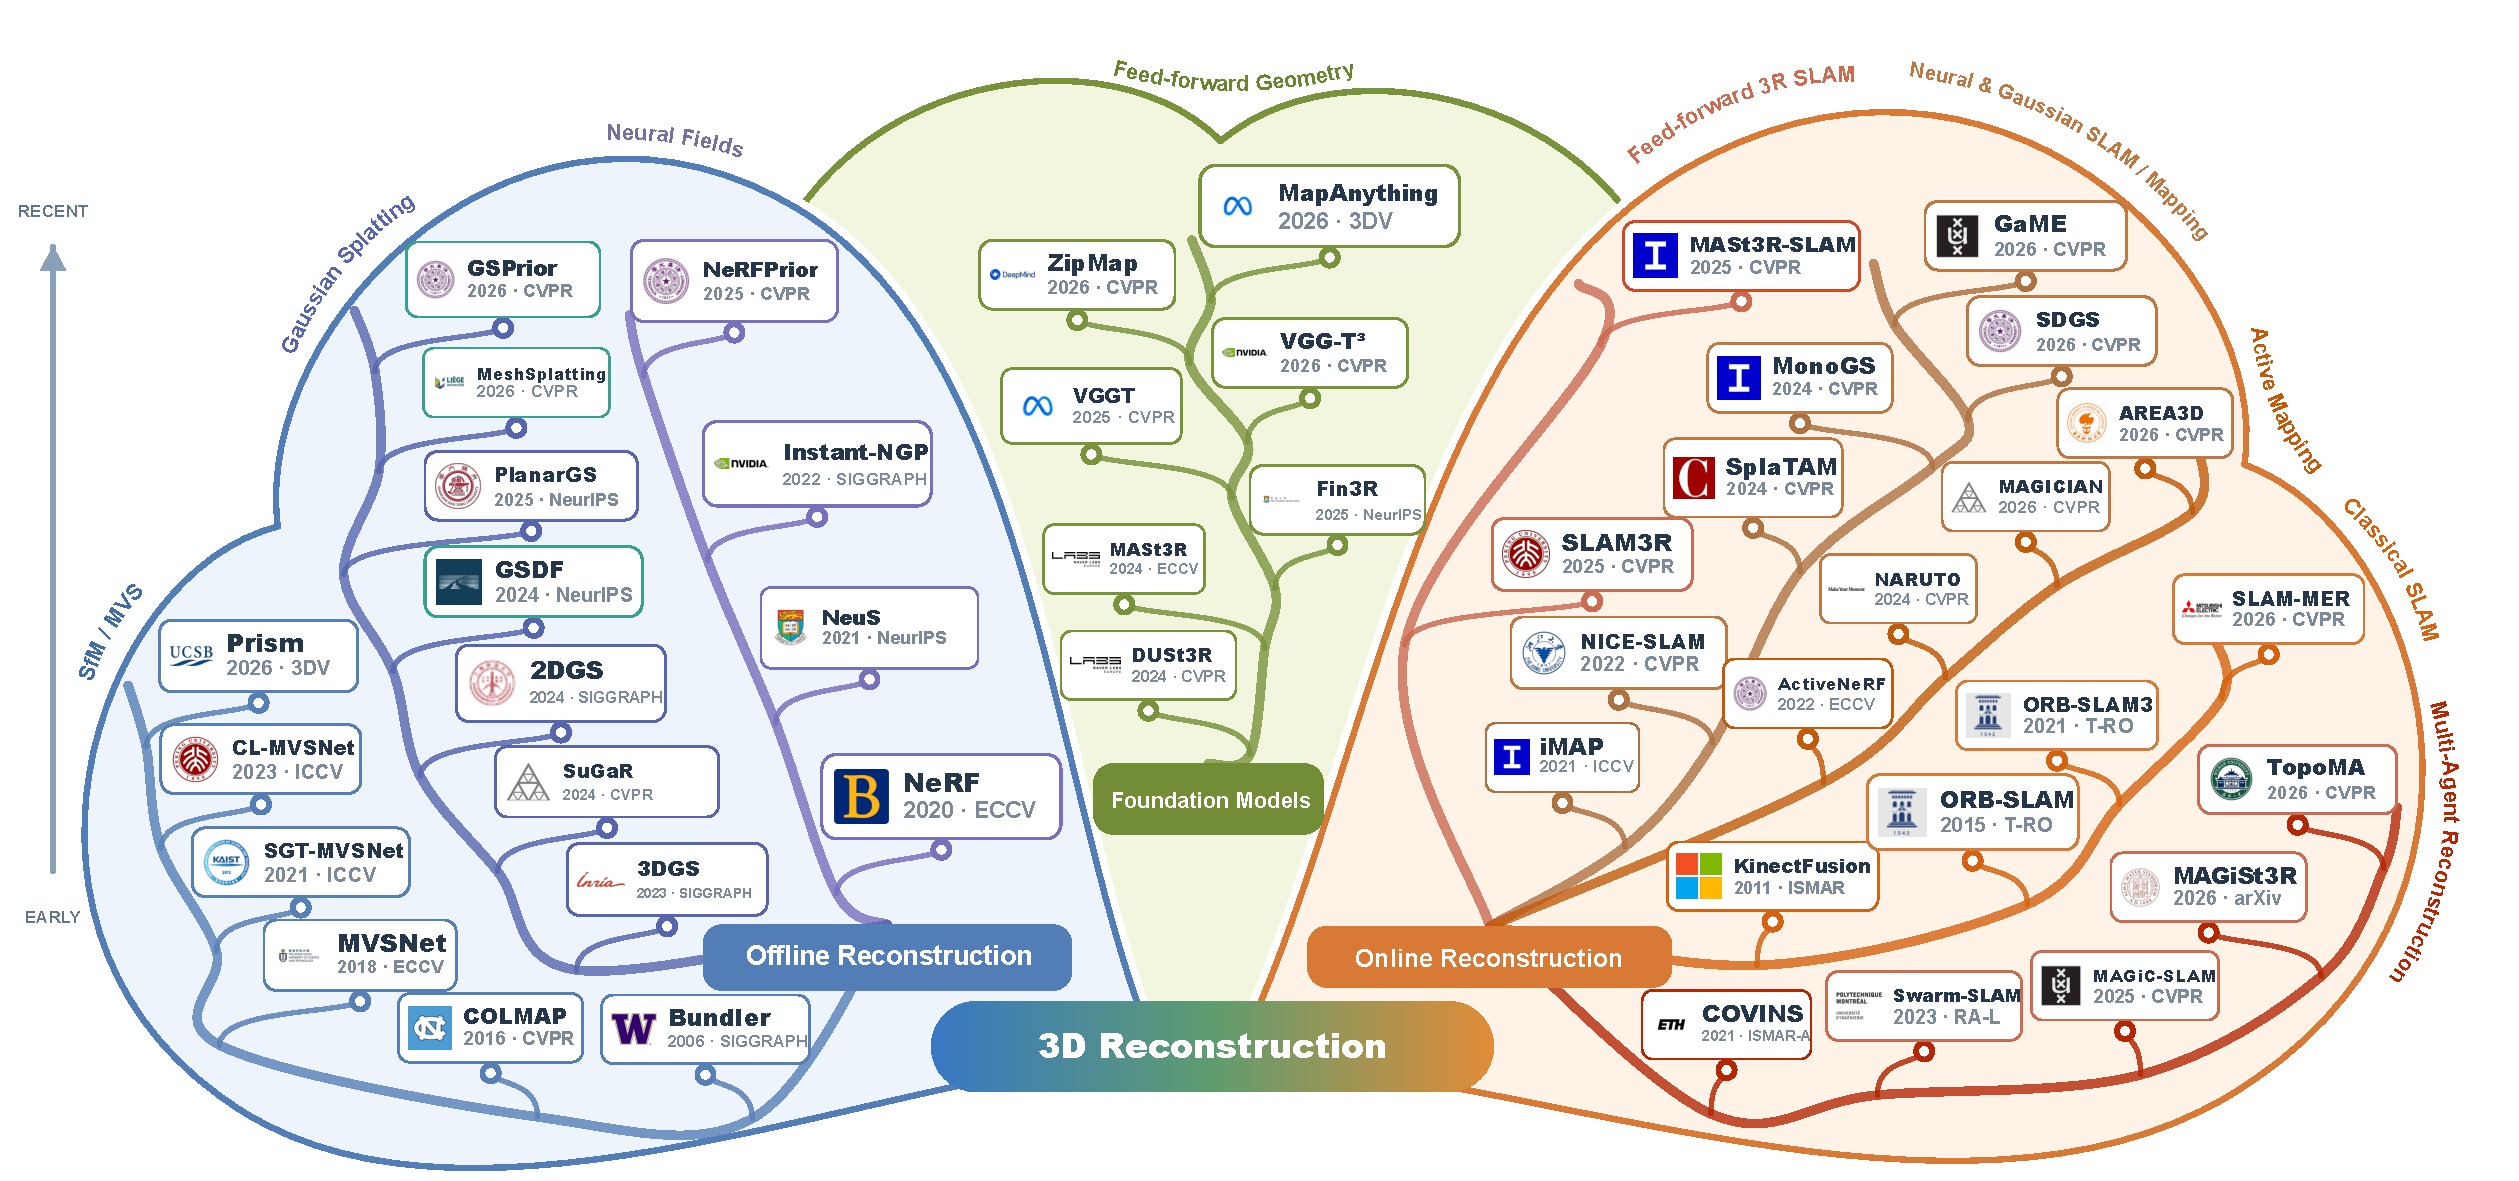
\includegraphics[width=\textwidth]{Figures/fig2.pdf}
    \caption{Taxonomy and chronological evolution of indoor scene reconstruction. Offline reconstruction, feed-forward reconstruction, and online reconstruction are organized as the three major paradigms, with representative methods arranged chronologically within their corresponding technical families.}
\label{fig:timeline}
\end{figure}
Indoor scene reconstruction provides an important spatial foundation for subsequent semantic understanding, physical reasoning, and embodied manipulation. Rather than viewing reconstruction methods as a single linear progression, we organize the literature into three complementary reconstruction paradigms that have emerged under different computational and deployment requirements: offline reconstruction, feed-forward geometry, and online reconstruction. Offline reconstruction estimates or optimizes a scene representation from a pre-collected set of observations, typically exploiting the full observation set to maximize geometric fidelity and completeness. Feed-forward geometry directly predicts scene geometry or 3D representations from one or more observations through a learned model in a forward inference pass, without relying on scene-specific optimization as the primary inference mechanism. Online reconstruction incrementally estimates camera pose and scene geometry as observations arrive during deployment, under joint constraints on accuracy, latency, memory, and computational resources. Fig.~\ref{fig:timeline} summarizes this taxonomy and orders representative methods chronologically within their corresponding technical families. The three paradigms should therefore be understood as complementary reconstruction regimes rather than as three strictly successive historical stages.

This organization highlights a fundamental trade-off in indoor scene reconstruction: offline methods can exploit extensive observations and scene-specific optimization for high-fidelity reconstruction, feed-forward methods prioritize rapid inference and generalization across unseen scenes, while online methods must additionally accommodate continuously arriving observations and limited computational resources. These differences in inference mechanisms and deployment requirements motivate distinct design choices in scene representation, optimization, and learning.

\subsection{Offline Reconstruction}
Offline reconstruction recovers scene geometry by optimizing a pre-collected set of observations, with an emphasis on geometric accuracy and completeness. Representative approaches have evolved from classical Structure from Motion (SfM) and Multi-View Stereo (MVS) to Neural Radiance Fields (NeRF) and 3D Gaussian Splatting (3DGS), reflecting fundamental changes in how scene geometry and appearance are represented and inferred. SfM and MVS recover camera poses and geometry through multi-view correspondence; NeRF represents scenes as continuous functions; and 3DGS models scenes as collections of explicit anisotropic 3D Gaussian primitives for efficient differentiable rendering. Despite substantial advances in reconstruction quality and efficiency, offline methods remain fundamentally constrained by the coverage and quality of the input observations, particularly in occluded, textureless, reflective, or otherwise poorly observed regions. Representative offline pipelines and outputs are illustrated in Fig.~\ref{fig:reconstruction_examples}(a), spanning learning-based MVS, neural implicit surface reconstruction, and surface-aligned Gaussian reconstruction.

\subsubsection{Structure from Motion (SfM)}
SfM jointly estimates camera poses and sparse scene geometry from image correspondences. Early systems such as Bundler~\cite{snavely2006photo} established scalable incremental reconstruction for unordered image collections, while COLMAP~\cite{schonberger2016structure} provided a robust and widely adopted pipeline integrating feature matching, geometric verification, camera registration, triangulation, and bundle adjustment. Despite their effectiveness on well-textured scenes, SfM methods remain sensitive to weak or repetitive textures, reflections, and other conditions that undermine reliable correspondence, which are particularly common in indoor environments. The consequence is not merely a lower aggregate accuracy: correspondence failure causes landmarks to disappear precisely on uniform walls, thin frames, and reflective appliances---structures that are directly relevant to contact and collision decisions. Moreover, the resulting sparse landmarks provide limited surface coverage, motivating dense reconstruction methods.

\subsubsection{Multi-View Stereo (MVS)}
MVS extends sparse SfM reconstruction by estimating dense depth or surface geometry from calibrated views~\cite{furukawa2015multiview}. Classical approaches rely on explicit correspondence propagation and geometric regularization~\cite{furukawa2010accurate}. PatchMatch propagation, introduced for binocular stereo~\cite{bleyer2011patchmatch} and subsequently extended to the multi-view setting, remains the representative formulation of this family. Learning-based methods instead learn feature representations and multi-view matching, with MVSNet~\cite{yao2018mvsnet} establishing a representative cost-volume formulation based on homography-warped features. These approaches improve robustness and data-driven regularization, but dense depth estimation remains sensitive to weak textures, occlusions, reflections, and domain shifts, while supervised training can require costly metric depth or 3D annotations. In textureless regions, the lack of reliable photometric evidence can make correspondence estimation ambiguous, causing the recovered geometry to rely more heavily on regularization or learned priors and potentially resulting in locally plausible but inaccurate surfaces. Such localized geometric errors can be particularly consequential for downstream embodied tasks that depend on precise surface geometry and contact relationships, even when scene-level reconstruction metrics remain competitive.

Reducing reliance on metric supervision has therefore become an important direction in learning-based MVS. Sparse-label approaches combine limited geometric supervision with multi-view consistency~\cite{kim2021just}, while self-supervised methods exploit photometric or cross-view constraints to avoid dense ground-truth depth~\cite{xu2021digging}. Contrastive learning further introduces image- and scene-level consistency to improve robustness in indistinguishable and view-dependent regions~\cite{xiong2025cl}. Recent methods instead strengthen the supervision signal itself: DIV Loss~\cite{rich2024smoothness} improves unsupervised training through depth smoothness, learned view synthesis, and additional supervisory views, while Prism~\cite{rich2026prism} combines unlabeled real videos with synthetic data and monocular structure priors to improve cross-domain generalization. These developments reduce dependence on dense metric labels, but do not remove the fundamental ambiguities caused by occlusion, weak texture, view-dependent appearance, and incomplete scene coverage. The remaining ambiguity is inherently unobservable from the provided images and is concentrated in exactly the regions---thin structures, glossy surfaces, occluded boundaries---that determine whether a subsequent grasp or contact query is valid.

\subsubsection{Neural Radiance Fields (NeRF)}
Neural implicit representations model scenes as continuous functions rather than discrete depth or point samples. NeRF~\cite{mildenhall2021nerf} represents a scene as a continuous 5D radiance field, where volume density is determined by the 3D position, while view-dependent radiance is conditioned on both the 3D position and viewing direction. Images are reconstructed through differentiable volume rendering. Although originally introduced for novel-view synthesis, the learned density field also provides implicit geometric cues for scene reconstruction. The density field does not, however, define a metrically meaningful surface, which motivates stronger surface constraints. Signed distance functions (SDFs) address this by defining the surface implicitly as their zero level set, so that geometry is represented by a single well-posed scalar field rather than recovered by thresholding density. Methods such as NeuS~\cite{wang2021neus} couple an SDF with volume rendering and formulate surface-aware density functions to recover geometrically coherent surfaces from multi-view observations.

For indoor reconstruction, subsequent methods further incorporate geometric priors to regularize neural fields in textureless, ambiguous, and occluded regions. ManhattanSDF~\cite{guo2022neural}, for example, exploits Manhattan-world constraints to improve the reconstruction of indoor structures, while NeRFPrior~\cite{zhang2025nerfprior} leverages radiance-field information to guide SDF-based surface reconstruction. Neural fields have also been extended beyond static geometry to dynamic scene modeling and appearance decomposition, as exemplified by D-NeRF~\cite{pumarola2021d}, K-Planes~\cite{fridovich2023k}, and NVDiffRec~\cite{munkberg2022extracting}. Meanwhile, efficient parameterizations such as NGLOD~\cite{takikawa2021neural}, Instant-NGP~\cite{muller2022instant}, and TensoRF~\cite{chen2022tensorf} substantially reduce the computational cost of neural field optimization and querying.
Despite these advances, neural radiance fields generally rely on scene-specific optimization and computationally intensive field evaluation, while explicit surface reconstruction often requires an additional surface extraction step. Two further limitations are specific to the implicit formulation. First, the density field is optimized to explain rendering rather than to define a surface, so its thresholded geometry is a byproduct of appearance fitting and can be systematically biased---inflated near boundaries or eroded on thin structures---even when rendered images look correct. Second, per-scene optimization makes the capture-to-model latency fundamentally incompatible with online embodied deployment unless inference is amortized. These limitations motivate the development of more efficient and explicit scene representations, leading to the emergence of 3D Gaussian Splatting as an alternative paradigm for scene reconstruction and rendering.

\subsubsection{3D Gaussian Splatting (3DGS)}

3D Gaussian Splatting (3DGS)~\cite{kerbl20233d} represents a scene as a set of anisotropic 3D Gaussian primitives with learnable geometry, opacity, and view-dependent appearance. Unlike NeRF, which relies on per-ray neural field evaluation and volume sampling, 3DGS employs differentiable splatting and rasterization, enabling efficient rendering and explicit manipulation of scene primitives. This explicit and highly parallel representation has made 3DGS an attractive alternative for large-scale and real-time scene reconstruction.

However, the key limitation of 3DGS is not rendering efficiency but state fidelity: photometric optimization can produce appearance-consistent Gaussian configurations without guaranteeing accurate contact geometry. For actionable scene understanding, the relevant representation is not the Gaussian field that best reproduces observed images, but the subset of geometry whose uncertainty is sufficiently constrained for collision, contact, and manipulation queries. This shifts the objective from photometric reconstruction toward task-conditioned geometric reliability. Indoor scenes contain textureless surfaces, reflective materials, and thin or irregular structures that can lead to poorly constrained Gaussian geometry. Recent methods therefore introduce surface, planar, normal, or SDF-based priors to improve geometric consistency, including GaussianShader~\cite{jiang2024gaussianshader}, PlanarGS~\cite{jin2025planargs}, GSDF~\cite{yu2024gsdf}, and PGSR~\cite{chen2024pgsr}. Other approaches explicitly align Gaussians with surfaces or reduce their volumetric nature, such as SuGaR~\cite{guedon2024sugar} and 2DGS~\cite{huang20242d}. These developments progressively shift 3DGS from a rendering-oriented representation toward a surface-aware scene representation.

Nevertheless, conventional 3DGS remains computationally and memory intensive because scene-specific optimization and densification can produce a large number of primitives. Compression, pruning, and level-of-detail strategies~\cite{niedermayr2024compressed} alleviate this burden, but efficient rendering, compact representation, and geometrically reliable reconstruction remain competing objectives. The more fundamental issue is that Gaussian parameters are optimized against photometric loss, so appearance can be explained by repositioning, splitting, or shaping primitives without a correspondingly correct surface; in textureless or specular regions, rendering metrics can therefore be high while the underlying geometry is wrong. For embodied applications, this distinction is particularly important: a visually plausible Gaussian representation must also provide sufficiently accurate and accessible geometry for collision, contact, and manipulation. These limitations motivate further research toward compact, geometrically grounded, and task-oriented scene representations.
\begin{figure}[!t]
    \centering
    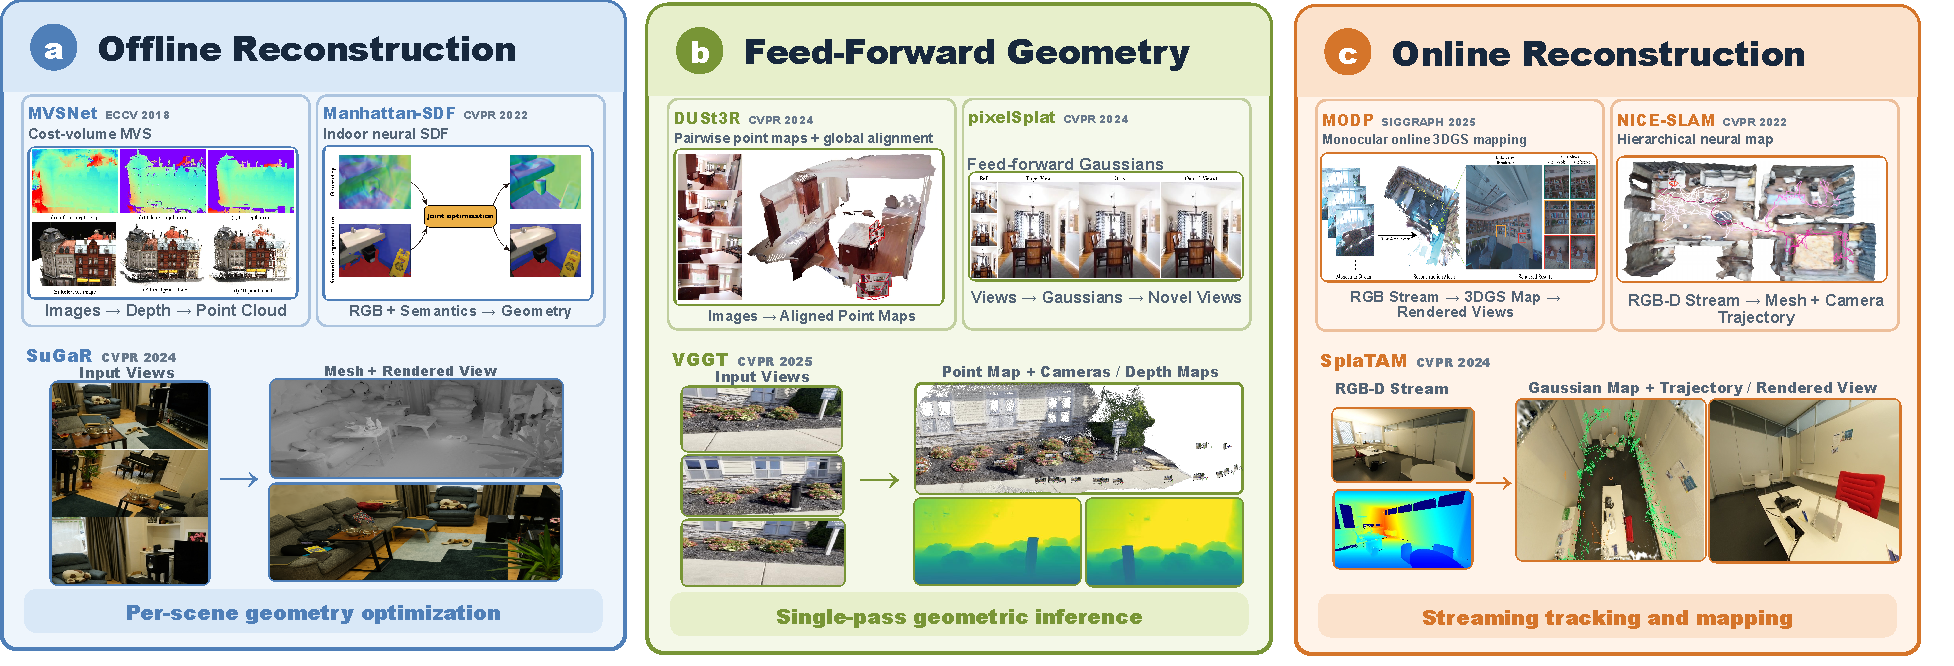
\includegraphics[width=\textwidth]{Figures/fig3v12.pdf}
    \caption{Representative examples of offline, feed-forward, and online 3D reconstruction paradigms.}
    \label{fig:reconstruction_examples}
\end{figure}



\subsection{Feed-Forward Geometry}
Feed-forward geometry is an inference regime rather than a self-contained mapping system. It responds to the latency and poor transferability of scene-specific optimization by amortizing geometric inference across training scenes and predicting geometry directly from new observations. As illustrated in Fig.~\ref{fig:reconstruction_examples}(b), representative feed-forward models directly produce aligned pointmaps, Gaussian primitives, or jointly estimated geometry and camera parameters from input images. This changes the central question from how to optimize one scene accurately to how to generalize geometric priors across scenes, cameras, view counts, and spatial scales. The boundary is not absolute: recent scalable or stateful models may update a compact latent representation through test-time training. Feed-forward geometry is therefore shown as the central bridge in Fig.~\ref{fig:timeline}: the same inference paradigm can process a pre-collected image set or supply rapid geometric priors to a streaming system, rather than constituting a third observation-acquisition mode alongside passive and active reconstruction.

\subsubsection{Pointmap-Based 3D Foundation Models}

Feed-forward 3D reconstruction aims to infer scene geometry and camera parameters directly from images, avoiding scene-specific optimization. DUSt3R~\cite{wang2024dust3r} establishes a pointmap-based formulation that predicts 3D points for image pairs in a common coordinate frame, while MASt3R~\cite{leroy2024grounding} improves cross-view matching by grounding correspondence in 3D. Subsequent foundation models extend this formulation to multi-view and more general geometric inference. VGGT~\cite{wang2025vggt} jointly predicts cameras, depths, pointmaps, and tracks, whereas MapAnything~\cite{keetha2026mapanything} unifies diverse visual and geometric inputs for metric 3D reconstruction and camera estimation. These models substantially reduce the cost of scene-specific reconstruction and provide strong geometric priors from sparse observations. However, feed-forward prediction alone does not guarantee global consistency or persistent scene state, particularly as the number of views increases or observations arrive over time. Because pointmap regression is trained with averaged prediction losses, the model tends to produce locally plausible geometry whose global consistency is only weakly constrained, and errors are not corrected by any subsequent alignment step. Its reliability outside the training distribution of camera configurations, view counts, and scene types therefore remains difficult to certify, which is a serious concern when the output is used to seed contact-level decisions.

\subsubsection{Scalable, Stateful, and Dynamic 3D Reconstruction}
The limitations of feed-forward pointmap prediction become more pronounced for fine-grained reconstruction, large image collections, and long or dynamic sequences. Fin3R~\cite{ren2025fin3r} improves geometric detail and robustness by distilling monocular geometric knowledge into feed-forward reconstruction models, addressing the limited fine-scale supervision and geometric misalignment of pointmap regression. ZipMap~\cite{jin2026zipmap} further introduces a stateful representation that compresses an image collection into a compact, queryable scene state, enabling linear-time reconstruction and streaming extensions. For dynamic scenes, D4RT~\cite{zhang2026efficiently} jointly models depth, spatio-temporal correspondence, and camera parameters and supports flexible 4D geometric queries. Together, these methods extend feed-forward reconstruction from instantaneous geometric prediction toward fine-grained, scalable, persistent, and dynamic scene modeling.

Despite their efficiency, feed-forward models are primarily designed for geometric inference from a given set of observations, rather than persistent scene maintenance. In embodied environments, however, the scene is continuously observed and must be incrementally updated while preserving spatial consistency over time. Stateful and streaming extensions such as ZipMap~\cite{jin2026zipmap} mitigate this gap by compressing observations into a queryable scene state, but compression itself introduces a fidelity--efficiency trade-off, and errors in the maintained state are propagated forward rather than corrected. This shifts the reconstruction objective from one-shot geometry estimation toward persistent spatial mapping, motivating online and active approaches for continuous scene registration, updating, and refinement.

\subsection{Online Reconstruction}

Online reconstruction incrementally builds and updates a scene representation as new observations arrive, requiring a balance among camera tracking, geometric accuracy, and computational efficiency. As illustrated by the representative neural and Gaussian systems in Fig.~\ref{fig:reconstruction_examples}(c), an incoming image stream is coupled with continuous camera tracking and incremental map updates. Existing approaches can be broadly categorized into classical SLAM, neural and Gaussian mapping, and feed-forward reconstruction integrated with SLAM. These paradigms mainly differ in how geometry is represented and how spatial consistency is maintained over time. For embodied applications, online reconstruction further needs to address three system-level challenges: selecting informative observations, coordinating multiple agents, and maintaining the scene representation under dynamic changes.

\subsubsection{Classical SLAM}

Classical SLAM emphasizes persistent camera localization and spatial consistency~\cite{cadena2016past}. Feature-based systems such as ORB-SLAM~\cite{mur2015orb} and ORB-SLAM3~\cite{campos2020orb} use sparse landmarks and geometric optimization for efficient tracking and loop closure, but provide limited dense surface geometry. RGB-D methods instead exploit direct depth observations to construct dense maps~\cite{dai2017bundlefusion}. KinectFusion~\cite{izadi2011kinectfusion} integrates depth into a TSDF volume, while DynamicFusion~\cite{newcombe2015dynamicfusion} extends volumetric reconstruction to non-rigid scenes. Hybrid approaches combine explicit localization with learned geometry, as exemplified by SLAM-MER~\cite{piedade2026revisiting}. Despite their robustness in spatial alignment, classical systems remain constrained by sensing quality, sparse observations, and the computational cost of dense mapping. Two of these limitations have distinct consequences for manipulation. Sparse-feature maps are optimized for tracking and place recognition, so they do not provide the dense, contact-ready surfaces needed for collision queries, while depth-based maps inherit sensor failures on transparent, reflective, and dark surfaces that are common in indoor scenes. Furthermore, drift accumulates over long trajectories and is only corrected at loop closure, so the local geometry that matters for a manipulation task may be the least reliable part of the map.

\subsubsection{Neural and Gaussian SLAM and Mapping}

Neural representations introduce continuous learned geometry into online mapping. iMAP~\cite{sucar2021imap}, NICE-SLAM~\cite{zhu2022nice}, and Vox-Fusion~\cite{yang2022vox} achieve dense reconstruction through neural scene representations, but repeated scene-specific optimization limits their scalability. Gaussian-based systems provide explicit primitives with efficient rendering, as demonstrated by MonoGS~\cite{matsuki2024gaussian} and SplaTAM~\cite{keetha2024splatam}. Subsequent methods improve geometric reliability through hierarchical representations and surface constraints, including MODP~\cite{wu2025MODP}, GPS-SLAM~\cite{peng2025gaussian}, and SDGS~\cite{tian2026sdgs}. Long-term mapping further requires handling environmental changes and outdated observations, as explored by GaME~\cite{yugay2026gaussian}. These methods improve map density and rendering efficiency, but optimization, memory consumption, and long-term map maintenance remain challenging. A subtler issue is that the map is optimized to explain the observations already received, so geometry in poorly observed regions is hallucinated in appearance-consistent but geometrically unreliable ways, and nothing in the optimization objective distinguishes ``unobserved'' from ``reconstructed''. Long-term maintenance also requires deletion, not only insertion: when an object is moved, the outdated geometry must be removed and the newly exposed free space updated, yet most mapping systems have no explicit mechanism for invalidating stale observations.

\subsubsection{Feed-Forward 3D Reconstruction with SLAM}

Feed-forward reconstruction provides strong geometric priors but does not inherently maintain a persistent global map. SLAM3R~\cite{liu2025slam3r} progressively registers local pointmaps, while MASt3R-SLAM~\cite{murai2025mast3r} integrates pointmap-based correspondence with loop closure and global optimization. This combination couples the efficiency of foundation-model inference with the spatial consistency of SLAM, reducing reliance on scene-specific optimization while retaining mechanisms for global correction. However, accurate reconstruction cannot compensate for insufficient scene coverage, motivating active observation strategies for embodied systems.

\subsubsection{Active Reconstruction}

Active reconstruction extends online mapping by controlling where observations are acquired. Rather than passively processing a camera stream, the system selects viewpoints that reduce geometric uncertainty or improve expected scene coverage. ActiveNeRF~\cite{pan2022activenerf} and NARUTO~\cite{feng2024naruto} perform next-best-view selection based on uncertainty estimates, while AREA3D~\cite{xu2026area3d} incorporates geometric uncertainty and vision--language guidance to select informative views. Beyond local uncertainty reduction, MAGICIAN~\cite{li2026magician} predicts unseen geometry to guide longer-horizon exploration. The central challenge is to balance immediate information gain with scene coverage, prediction reliability, and exploration cost. In practice, uncertainty estimates are model-relative and often miscalibrated, so a view that maximizes predicted information gain may not reduce true reconstruction error; moreover, information gain for reconstruction is not the same as information gain for the task, and a next-best view that improves global coverage may still leave the grasp-relevant region of a target object poorly observed.

\subsubsection{Multi-Agent Reconstruction}

Multi-agent reconstruction extends online mapping across multiple sensing platforms, increasing spatial coverage while introducing coordination and communication constraints. Centralized systems such as COVINS~\cite{schmuck2021covins} perform global place recognition and optimization through a shared backend, whereas decentralized systems such as Swarm-SLAM~\cite{lajoie2023swarm} distribute estimation across agents. Recent approaches exchange denser learned representations, including neural points~\cite{hu2023cp}, neural maps~\cite{deng2025mne}, and Gaussian primitives~\cite{yugay2025magic}. Feed-forward geometric priors can further reduce local reconstruction cost and facilitate compact cross-agent information exchange. Nevertheless, globally consistent reconstruction still depends on reliable place recognition, coordinate alignment, submap fusion, and communication-efficient optimization. Compression for communication introduces a trade-off between geometric fidelity and bandwidth, and place recognition itself degrades under changing illumination or appearance, so the assumed overlap between agents may not be detectable in practice. The coordination gain is therefore contingent on conditions that the reconstruction system itself cannot control.

\subsubsection{Dynamic and Action-Induced Reconstruction}

Scene dynamics introduce a further challenge because previously reconstructed geometry may become invalid after object motion or physical interaction. Existing approaches model time-varying geometry through deformation fields, factorized space--time representations, deformable Gaussians, and feed-forward 4D prediction~\cite{newcombe2015dynamicfusion,pumarola2021d,fridovich2023k,yang2024deformable,luiten2024dynamic,zhang2026efficiently}. For embodied manipulation, however, the challenge extends beyond modeling observed motion: the system must detect state changes, update affected geometry and free space, and preserve spatial consistency for subsequent actions. Most dynamic reconstruction methods model motion that is already visible; they do not distinguish action-induced, semantically meaningful state changes from noise, nor do they propagate the consequences of a change to occluded regions that were never observed after the event. Dynamic reconstruction therefore shifts the objective from modeling temporal variation to maintaining an actionable spatial state under continuous change.

Overall, online reconstruction is evolving from passive map maintenance toward adaptive spatial perception. Classical SLAM provides persistent geometric alignment, neural and Gaussian methods enrich scene representations, and feed-forward models reduce reconstruction latency. Active, multi-agent, and dynamic extensions further determine how observations are acquired, coordinated, and incorporated into the scene representation under changing environments, bringing reconstruction closer to the persistent and task-aware spatial representations required by embodied systems. Across all three paradigms, however, the evaluation gap remains: reconstruction benchmarks report Chamfer distance, F-scores, and rendering fidelity averaged over whole scenes, none of which measures whether the geometry supports a collision query, a contact planning request, or a grasp selection. As a result, a method can score well on reconstruction benchmarks while producing geometry that fails precisely at the interaction-relevant locations where embodied systems depend on it. Closing this gap requires task-conditioned evaluation in which reconstructed maps are consumed by downstream geometric queries and manipulation planning, not merely compared with ground-truth surfaces.

\section{Semantic Understanding}
\label{sec:semantic_understanding}
\begin{figure}[!t]
    \centering
    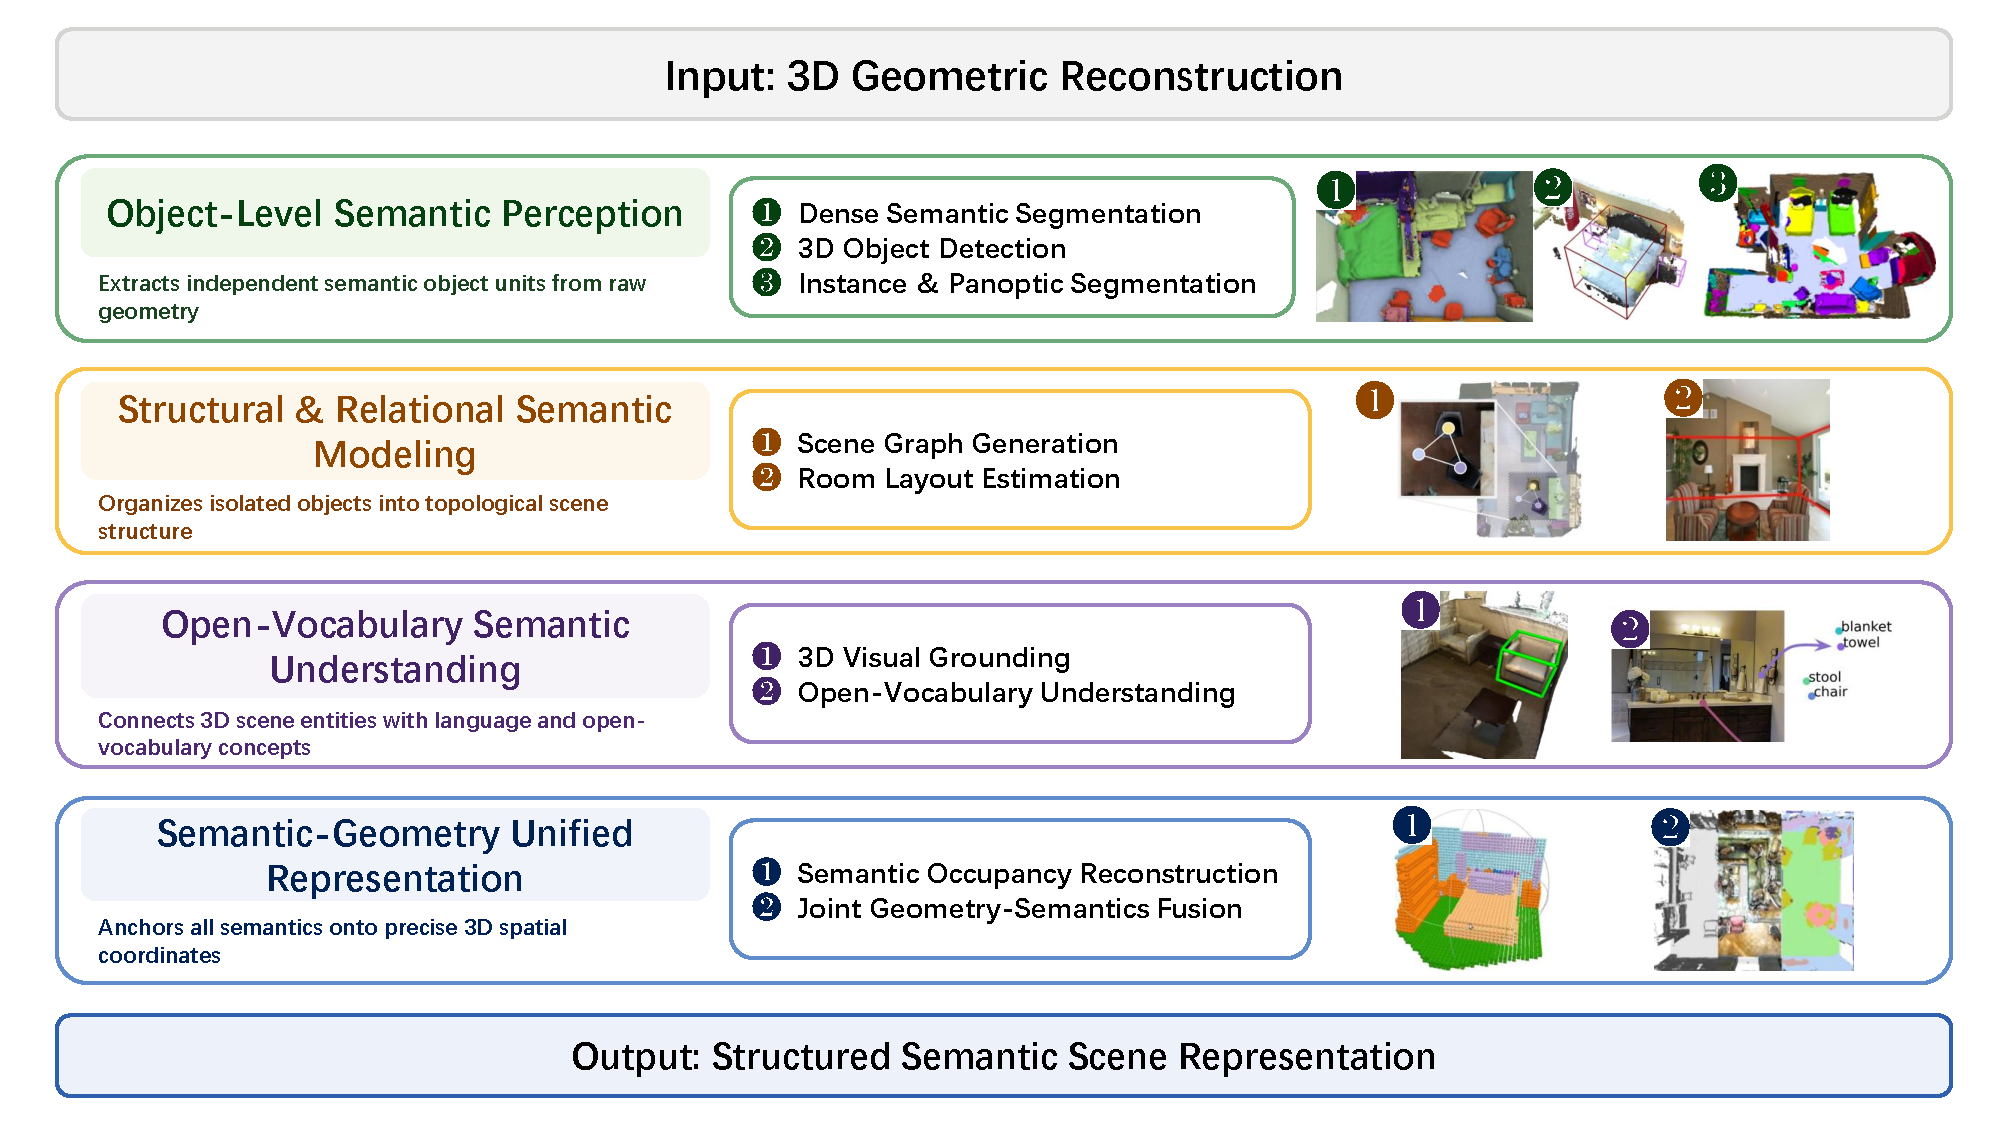
\includegraphics[width=1\linewidth]{Figures/semantic_evo.pdf}
    \caption{The four-layer bottom-up framework progressively transforms reconstructed 3D geometry into structured semantic representations, evolving from object-level perception and relational modeling to open-vocabulary semantic understanding and unified geometry--semantic representation. It establishes the semantic foundation for subsequent physical and functional reasoning, thereby bridging geometric scene reconstruction and actionable scene understanding for embodied manipulation.}
    \label{fig:placeholder}
\end{figure}

\newcommand{\posbar}{\textcolor{green!55!black}{\rule{1.2pt}{8.0pt}}\;}
\newcommand{\negbar}{\textcolor{red!70!black}{\rule{1.2pt}{8.0pt}}\;}
\newcommand{\prog}{\textcolor{black!45}{\(\rightarrow\)}}

\begin{table}[!t]
\centering
\scriptsize
\setlength{\tabcolsep}{3pt}
\renewcommand{\arraystretch}{1.30}

\caption{Comparison of Semantic Understanding Paradigms for Indoor Scene Reconstruction.
Each paradigm targets a distinct level of structural abstraction, from pixel-wise labeling to language-grounded scene modeling.
}
\label{tab:semantic_paradigms}
\vspace{0.4em}

\rowcolors{2}{lightBlue!18}{white}

\begin{tabularx}{\textwidth}{
>{\raggedright\arraybackslash}p{1.85cm}
>{\raggedright\arraybackslash}p{1.5cm}
>{\raggedright\arraybackslash}p{3.5cm}
>{\raggedright\arraybackslash\setlength{\parindent}{0pt}}X
>{\raggedright\arraybackslash\setlength{\parindent}{0pt}}X
>{\centering\arraybackslash}p{1.45cm}
>{\centering\arraybackslash}p{1.3cm}
}
\toprule
\rowcolor{TableNavy}
\multicolumn{1}{c}{\textcolor{white}{\bfseries Category}} &
\multicolumn{1}{c}{\textcolor{white}{\bfseries Core Task}} &
\multicolumn{1}{c}{\textcolor{white}{\bfseries Representative Methods}} &
\multicolumn{1}{c}{\textcolor{white}{\bfseries Strengths}} &
\multicolumn{1}{c}{\textcolor{white}{\bfseries Limitations}} &
\multicolumn{1}{c}{\textcolor{white}{\bfseries Output}} &
\multicolumn{1}{c}{\makecell{\textcolor{white}{\bfseries Action}\\\textcolor{white}{\bfseries relevance}}} \\
\midrule

\renewcommand{\arraystretch}{1.20}

Semantic Segmentation &
Pixel-/\allowbreak{}point-level label prediction &
PointNet++~\cite{qi2017pointnet++}, KPConv~\cite{thomas2019kpconv}, StratifiedTF~\cite{lai2022stratified}, PointNeXt~\cite{qian2022pointnext}, PTv3~\cite{wu2024point}, Swin3D~\cite{yang2025swin3d} &
{\posbar \textcolor{green!55!black}{\bfseries +}\, Establishes dense semantic basis\par
\posbar \textcolor{green!55!black}{\bfseries +}\, Hierarchical \& local feature learning\par
\posbar \textcolor{green!55!black}{\bfseries +}\, Backbone for downstream tasks} &
{\negbar \textcolor{red!70!black}{\bfseries --}\, No instance distinction\par
\negbar \textcolor{red!70!black}{\bfseries --}\, Limited relational understanding\par
\negbar \textcolor{red!70!black}{\bfseries --}\, Closed-set categories} &
semantic label &
low \\
\addlinespace[2pt]

Instance/\newline Panoptic Segmentation &
Object-level mask prediction &
3D-BoNet~\cite{yang2019learning}, HAIS~\cite{chen2021hais}, SoftGroup~\cite{vu2022softgroup}, Mask3D~\cite{schult2023mask3d}, OneFormer3D~\cite{kolodiazhnyi2024oneformer3d}, Pano3D~\cite{barberteguy2026pano3d} &
{\posbar \textcolor{green!55!black}{\bfseries +}\, Object-aware reasoning\par
\posbar \textcolor{green!55!black}{\bfseries +}\, Unified ``things'' \& ``stuff'' modeling\par
\posbar \textcolor{green!55!black}{\bfseries +}\, End-to-end mask prediction} &
{\negbar \textcolor{red!70!black}{\bfseries --}\, Occlusion handling\par
\negbar \textcolor{red!70!black}{\bfseries --}\, Over-segmentation\par
\negbar \textcolor{red!70!black}{\bfseries --}\, Post-processing still needed} &
instance mask &
low-medium \\
\addlinespace[2pt]

3D Object Detection &
Bounding-box localization &
VoteNet~\cite{qi2019deep}, FCAF3D~\cite{rukhovich2022fcaf3d}, CAGroup3D~\cite{wang2022cagroup3d}, TR3D~\cite{rukhovich2023tr3d}, SPGroup3D~\cite{zhu2024spgroup3d}, Cubify Anything~\cite{lazarow2025cubify} &
{\posbar \textcolor{green!55!black}{\bfseries +}\, Compact representation\par
\posbar \textcolor{green!55!black}{\bfseries +}\, Query-driven\par
\posbar \textcolor{green!55!black}{\bfseries +}\, RGB-D multimodal fusion} &
{\negbar \textcolor{red!70!black}{\bfseries --}\, Coarse geometry\par
\negbar \textcolor{red!70!black}{\bfseries --}\, Bbox not sufficient for interaction\par
\negbar \textcolor{red!70!black}{\bfseries --}\, Small-object recall} &
object location &
medium \\
\addlinespace[2pt]

Scene Graph Generation &
Relational structure learning &
Neural Motifs~\cite{zellers2018neural}, SceneGraph-Fusion~\cite{Wu2021}, SGFormer~\cite{lv2024sgformer}, SDSGG~\cite{chen2024sdsgg}, SceneLLM~\cite{zhang2026scenellm} &
{\posbar \textcolor{green!55!black}{\bfseries +}\, Relational reasoning\par
\posbar \textcolor{green!55!black}{\bfseries +}\, Hierarchical scene modeling\par
\posbar \textcolor{green!55!black}{\bfseries +}\, Embodied planning support} &
{\negbar \textcolor{red!70!black}{\bfseries --}\, Long-tail relations\par
\negbar \textcolor{red!70!black}{\bfseries --}\, Scalability issues\par
\negbar \textcolor{red!70!black}{\bfseries --}\, Noise in cluttered scenes} &
relations &
medium-high \\
\addlinespace[2pt]

Layout Estimation &
Room structure recovery &
HorizonNet~\cite{Sun2019HorizonNet}, LED2-Net~\cite{Wang2021LED2}, Bi-Layout~\cite{Tsai2024BiLayout}, uLayout~\cite{Lee2025uLayout}, Plane-DUSt3R~\cite{Huang2025PlaneDUSt3R} &
{\posbar \textcolor{green!55!black}{\bfseries +}\, Structural prior\par
\posbar \textcolor{green!55!black}{\bfseries +}\, Topological reasoning\par
\posbar \textcolor{green!55!black}{\bfseries +}\, Supports navigation and planning} &
{\negbar \textcolor{red!70!black}{\bfseries --}\, Manhattan-world assumption\par
\negbar \textcolor{red!70!black}{\bfseries --}\, Cluttered-scene fragmentation\par
\negbar \textcolor{red!70!black}{\bfseries --}\, Limited to rooms} &
room layout &
medium \\
\addlinespace[2pt]

3D Visual Grounding &
Language-grounded object localization &
ScanRefer~\cite{chen2020scanrefer}, Instance-Refer~\cite{yuan2021instancerefer}, 3DVG-Transformer~\cite{zhao20213dvgtransformer}, LanguageRefer~\cite{roh2021languagerefer}, 3D-VisTA~\cite{zhu20233dvista}, LL3DA~\cite{chen2024ll3da} &
{\posbar \textcolor{green!55!black}{\bfseries +}\, Open-ended queries\par
\posbar \textcolor{green!55!black}{\bfseries +}\, Spatial-language alignment\par
\posbar \textcolor{green!55!black}{\bfseries +}\, Embodied instruction interface} &
{\negbar \textcolor{red!70!black}{\bfseries --}\, Referring-expression ambiguity\par
\negbar \textcolor{red!70!black}{\bfseries --}\, Reliance on reconstruction quality\par
\negbar \textcolor{red!70!black}{\bfseries --}\, Annotation cost} &
task-conditioned entity &
high \\
\addlinespace[2pt]

Semantic Geometry Reconstruction &
Geometry-semantics joint modeling &
SSCNet~\cite{song2017sscnet}, Scan-Complete~\cite{dai2018scancomplete}, SemanticNeRF~\cite{zhi2021semanticnerf}, SemanticFusion~\cite{mccormac2017semanticfusion} &
{\posbar \textcolor{green!55!black}{\bfseries +}\, Continuous field rep.\par
\posbar \textcolor{green!55!black}{\bfseries +}\, Navigable space\par
\posbar \textcolor{green!55!black}{\bfseries +}\, Multi-task unified framework} &
{\negbar \textcolor{red!70!black}{\bfseries --}\, High memory cost\par
\negbar \textcolor{red!70!black}{\bfseries --}\, Sparse supervision\par
\negbar \textcolor{red!70!black}{\bfseries --}\, Resolution trade-off} &
spatial semantic state &
high \\
\bottomrule


\end{tabularx}

\renewcommand{\arraystretch}{1.15}

\end{table}

Section~\ref{sec:geometric_reconstruction} reconstructed the geometry of the environment and established \emph{where} entities are located. Geometry alone, however, does not specify \emph{what} these entities are, how they are organized and related, or how they can be identified through natural language. Semantic understanding therefore enriches reconstructed geometry with structured and interpretable meaning, providing the semantic foundation for the physical and functional reasoning developed in subsequent sections. It is worth noting at the outset that semantic accuracy, as measured by benchmarks, is not identical to semantic utility: a label that is correct at the category level can still be useless for interaction if it does not capture the state, parts, or accessibility of the labeled entity, and every semantic error is compounded by the errors of the reconstruction from which it is computed.

Rather than treating semantic understanding as a collection of independent recognition tasks, this section organizes existing methods according to progressively richer forms of scene semantics, as outlined in Fig.~\ref{fig:placeholder} and compared in Table~\ref{tab:semantic_paradigms}. For each paradigm, the table juxtaposes representative methods, strengths, and limitations with the output representation it delivers and its action relevance, i.e., how directly that output can support downstream manipulation. The action relevance rises from \emph{low} for pixel-level semantic labels, through \emph{medium} for object locations and \emph{medium-high} for relational structures, to \emph{high} for task-conditioned grounding and spatial semantic states, mirroring the progression of the taxonomy itself. The taxonomy proceeds from \emph{object-level semantic units}, through \emph{scene-level relational structures} and \emph{language-grounded semantics}, to \emph{geometry--semantic unified representations}. The first three levels progressively enrich the semantic description of scene entities and their relations, whereas the fourth binds these semantics back to the underlying spatial representation. This progression extends the scene representation from purely geometric structure $\mathcal{G}$ to a joint geometry--semantic representation $\{\mathcal{G},\mathcal{S}\}$, establishing the semantic basis for subsequent physical, functional, and affordance reasoning. Each subsection therefore focuses on the representation provided at its corresponding level and the limitations that motivate the next.

\subsection{Object-Level Semantic Perception}

Object-level semantic perception assigns semantic identities to geometric elements and organizes them into meaningful entities. It provides the basic units for subsequent relational and language-based reasoning. Three closely related tasks form the conventional hierarchy: semantic segmentation assigns category labels to spatial elements; instance and panoptic segmentation further distinguish individual object instances and background regions; and 3D object detection represents objects with compact geometric hypotheses such as bounding boxes. These tasks differ in output granularity but share the goal of transforming unstructured 3D geometry into structured semantic entities~\cite{guo2020deep}. As the first three rows of Table~\ref{tab:semantic_paradigms} show, their outputs---semantic labels, instance masks, and object locations---also differ in action relevance, from low to medium, reflecting how directly each representation identifies an entity that a manipulation policy could target.

Large-scale indoor datasets, including ScanNet~\cite{dai2017scannet}, S3DIS~\cite{armeni2017joint}, and Matterport3D~\cite{chang2017matterport3d}, have provided the principal benchmarks for learning and evaluating object-level semantics. Methodologically, 3D semantic segmentation has evolved from point-based local feature aggregation toward architectures capable of modeling larger spatial contexts~\cite{choy20194d}. PointNet++~\cite{qi2017pointnet++} introduced hierarchical local feature learning for irregular point sets, while KPConv~\cite{thomas2019kpconv} improved geometric feature extraction through deformable kernel operators. PointNeXt~\cite{qian2022pointnext} subsequently showed that improvements in training strategies and architectural scaling can substantially strengthen point-based baselines. Transformer-based approaches further enlarge the effective receptive field through stratified attention~\cite{lai2022stratified}, serialized point representations~\cite{wu2024point}, and hierarchical attention over sparse 3D voxels~\cite{yang2025swin3d}. The resulting progression reflects a broader shift from local geometric labeling toward context-aware semantic modeling in cluttered indoor environments.

Instance and panoptic segmentation extend category prediction to object-level identity. Early approaches rely on point grouping or proposal generation~\cite{jiang2020pointgroup}, with methods such as 3D-BoNet~\cite{yang2019learning} and HAIS~\cite{chen2021hais} progressively improving instance formation through point aggregation and hierarchical grouping. SoftGroup~\cite{vu2022softgroup} reduces the dependence on hard semantic assignments, while Mask3D~\cite{schult2023mask3d} adopts learnable queries for end-to-end instance mask prediction. OneFormer3D~\cite{kolodiazhnyi2024oneformer3d} further unifies semantic, instance, and panoptic segmentation within a common query-based framework. Recent work also explores joint reconstruction and panoptic prediction~\cite{barberteguy2026pano3d}, indicating increasing integration between geometric recovery and semantic interpretation.

3D object detection provides a more compact representation by associating each object with a localized geometric hypothesis. Early point-based detectors rely on geometric voting and local aggregation~\cite{qi2019deep}; subsequent anchor-free approaches remove predefined proposal structures~\cite{rukhovich2022fcaf3d}, while semantic-guided grouping~\cite{wang2022cagroup3d}, superpoint-based aggregation~\cite{zhu2024spgroup3d}, and Transformer-based detection~\cite{rukhovich2023tr3d} progressively improve contextual modeling and efficiency. Recent approaches further demonstrate that large-scale pre-training can support 3D detection from RGB or RGB-D observations without relying exclusively on conventional point- or voxel-based representations~\cite{lazarow2025cubify}. Multimodal methods additionally combine appearance and geometry through cross-modal attention and feature fusion~\cite{cheng2023tbfnt3d}, improving robustness to ambiguous appearance and incomplete geometry.

Taken together, semantic segmentation, instance and panoptic segmentation, and object detection transform reconstructed geometry into semantic entities with category, identity, and spatial extent. Their outputs differ in granularity and structure, but none explicitly describes how these entities are organized within a scene. More importantly, benchmark evaluation of these tasks is largely decoupled from the interaction requirements they are meant to serve. Category vocabularies are closed and defined by annotation cost rather than functional relevance: a mug, a lamp, and a window may all be labeled correctly while their manipulable parts, current state, and accessibility remain unspecified. Semantic labels are also static snapshots: instance identity is not preserved across observations, and state changes such as an opened drawer or a displaced object are invisible to a per-frame label. Finally, object-level outputs inherit every error of the underlying reconstruction; on incomplete or drifted geometry, segmentation boundaries and detection boxes are systematically biased, so semantic accuracy on clean benchmark scans does not guarantee reliability on live reconstruction. This limitation motivates relational semantic modeling at the scene level.

\subsection{Relational Semantic Modeling}

Object-level semantics provide the entities of a scene but not the structure that connects them. Relational modeling therefore organizes objects, regions, and rooms through spatial, semantic, and functional relations, while room layout estimation provides complementary structural information at a larger spatial scale. Together, these representations describe how entities are embedded within the surrounding scene rather than treating them as independent predictions.

3D scene graph generation has evolved from local relational prediction toward increasingly structured and language-aware representations. Early systems use graph neural networks to aggregate object and point features and predict semantic relations~\cite{Wu2021}. Transformer-based approaches introduce broader contextual reasoning and language priors, as exemplified by SGFormer~\cite{lv2024sgformer}, while open-vocabulary and language-model-based methods extend the relation space beyond predefined predicates~\cite{chen2024sdsgg}. Hierarchical representations further organize objects within regions and rooms, providing a structured description of indoor environments~\cite{armeni20193d}. Generative approaches such as Graph2Scene~\cite{chen2025graph2scene} additionally demonstrate that scene graphs can serve as structured conditions for scene generation, extending their role beyond passive semantic description.

Room layout estimation complements object relations by recovering large-scale structural elements such as walls, floors, ceilings, doorways, and room connectivity~\cite{zou2018layoutnet}. Early methods formulate layout recovery as boundary or depth estimation in panoramic images~\cite{Sun2019HorizonNet,Wang2021LED2}. Subsequent approaches explicitly model structural relations among walls~\cite{jiang2022lgt}, generate parameterized layouts through query-based prediction~\cite{mia2026layout}, and represent room structures using topological graphs~\cite{yao2023undirected}. Unified models further address variation across perspective and panoramic observations~\cite{Lee2025uLayout}, while recent foundation-model-based methods infer layout structure directly from sparse views~\cite{Huang2025PlaneDUSt3R}.

Scene graphs and layout representations capture complementary scales of spatial organization: scene graphs specify relations among semantic entities, whereas layouts describe the structural and topological organization of the surrounding space. Their combination provides a richer scene-level representation for subsequent semantic querying and reasoning. However, these representations remain largely dependent on predefined semantic vocabularies or relation types, limiting their ability to interpret open-ended natural-language descriptions. Two further limitations are specific to relational modeling. First, relation prediction on benchmarks is strongly driven by category co-occurrence statistics, so a large share of the measured gain can reflect prior fitting rather than genuine relational understanding, especially for the frequent relations that dominate evaluation. Second, scene graphs and layouts are typically built once from a static scan and are not updated as objects move or states change, which restricts their use in interactive settings. This motivates language-grounded semantic understanding.

\subsection{Language-Grounded Semantics}
Natural language provides a flexible interface for specifying entities, attributes, relations, and spatial references that may not be captured by fixed semantic labels. Language-grounded scene understanding therefore aligns textual descriptions with reconstructed 3D entities and regions, enabling semantic querying beyond predefined category sets. Two closely related directions are 3D visual grounding, which localizes language expressions in a reconstructed scene, and open-vocabulary 3D understanding, which extends semantic prediction beyond closed label spaces.

3D visual grounding is typically evaluated on reconstructed indoor environments. ScanRefer~\cite{chen2020scanrefer} introduced natural-language descriptions for objects in ScanNet, while ReferIt3D~\cite{achlioptas2020referit3d} established the Nr3D and Sr3D benchmarks with greater emphasis on spatial and attribute reasoning. Multi3DRefer~\cite{zhang2023multi3drefer} extended grounding to descriptions referring to multiple objects, and ScanQA~\cite{azuma2022scanqa} formulated language-conditioned question answering over 3D scenes. Methodologically, early approaches rely on candidate object proposals followed by language--geometry matching~\cite{chen2020scanrefer,yuan2021instancerefer}. Subsequent models incorporate pairwise attention and spatial-language reasoning~\cite{zhao20213dvgtransformer,roh2021languagerefer}, while 3D vision-language models such as 3D-VisTA~\cite{zhu20233dvista} learn transferable scene--language representations across grounding, question answering, and captioning. LLM-based systems such as 3D-LLM and LL3DA~\cite{hong20233dllm,chen2024ll3da} further broaden the interaction space by mapping 3D scene representations into instruction-following language models.

In parallel, open-vocabulary methods relax the dependence on predefined semantic categories. Vision-language pre-training, exemplified by CLIP~\cite{radford2021clip}, provides a general mechanism for aligning visual or geometric features with textual concepts. OpenScene~\cite{peng2023openscene} and related approaches transfer such language-aligned representations to 3D space, while open-vocabulary occupancy methods integrate semantic categories into spatial representations~\cite{jiang2024openocc}. Other methods extend language alignment to scene graphs and dense multimodal representations~\cite{werby2024hierarchical,li2024dense}, enabling semantic descriptions at object, region, and attribute levels.

These developments shift 3D semantic understanding from closed-set recognition toward language-grounded and open-vocabulary interpretation. Nevertheless, language alignment remains meaningful only when textual semantics can be accurately associated with the underlying geometry. Grounding is currently evaluated on offline reconstructed scans with clean geometry and fixed viewpoints, which masks the errors that arise when the same task is performed on live, incomplete reconstruction. Referring expressions are also inherently ambiguous and underspecified, so benchmark accuracy partly measures how well a model guesses among plausible referents, and open-vocabulary features inherit 2D biases in scale, viewpoint, and occlusion without being spatially precise by construction. This requirement motivates a unified representation in which semantic information and spatial structure are jointly maintained.

\subsection{Geometry--Semantic Unified Representation}

The preceding levels progressively identify semantic entities, organize their relations, and align them with open-ended language. A geometry--semantic unified representation integrates these semantic attributes directly with the reconstructed spatial representation, allowing geometric and semantic information to be queried within a common coordinate system. Unlike the preceding levels, which primarily enrich the semantic description of reconstructed geometry, this level concerns the joint representation of \emph{where} and \emph{what} at each spatial location.

Occupancy-based representations provide a natural formulation for this integration by associating spatial locations with both geometric occupancy and semantic labels~\cite{cao2022monoscene}. Indoor semantic scene completion instantiates this formulation directly: SSCNet~\cite{song2017sscnet} infers complete geometry and per-voxel semantic labels from a single depth frame of an indoor scene, while ScanComplete~\cite{dai2018scancomplete} extends completion and semantic labeling to large, partially observed 3D scans through coarse-to-fine inference. Neural reconstruction further binds semantics into the underlying representation: SemanticNeRF~\cite{zhi2021semanticnerf} couples implicit geometry with per-point semantic fields under multi-view consistency constraints, whereas SemanticFusion~\cite{mccormac2017semanticfusion} fuses frame-level semantic predictions into dense RGB-D maps and thereby improves the consistency and coverage of scene-wide labeling from limited observations. Open-vocabulary extensions further attach language-aligned semantics directly to reconstructed geometry rather than restricting labels to a closed category set~\cite{takmaz2023openmask3d}, as exemplified by ConceptFusion~\cite{javatavallabhula2023conceptfusion}. Instance-aware systems additionally preserve object identity within the joint representation: Fusion++~\cite{mccormac2018fusionpp} maintains object-level volumetric maps with semantic and instance labels, providing persistent per-object spatial support for subsequent interaction.

The importance of geometry--semantic binding lies in its ability to preserve semantic identity together with spatial correspondence. A category label without reliable spatial support cannot determine the location or extent of an entity, while geometry without semantics cannot distinguish among entities or support semantic queries. Joint representations therefore provide a more complete description of indoor environments and establish a common spatial basis for the physical and functional attributes considered in the next section. Their limitations are equally instructive. Occupancy formulations discretize space, so semantic resolution is bounded by voxel resolution and memory, and labels are available only where supervision exists---typically on observed surfaces---leaving most of the volume semantically undetermined. The representation is also static: state changes require re-inference over the affected region rather than a local, incremental update. Most fundamentally, binding semantics to geometry specifies what occupies a location but not whether it can be interacted with, so the joint representation remains a necessary rather than sufficient condition for actionable understanding.

Overall, the four levels progressively enrich the scene representation from semantic entities, to relational scene structure, to language-grounded semantics, and finally to geometry--semantic binding. This progression extends the reconstructed geometry into a structured semantic representation that incorporates both geometric and semantic information. Nevertheless, semantic richness alone does not establish actionability. Semantic understanding for embodied manipulation must move from recognizing what an object is to maintaining which instance it is, where it is, what state it is in, and which task-relevant region can be acted upon. This naturally motivates the integration of semantic representations with the physical and functional information discussed in the next section.

% ================================
% 表格配置与定义（放在导言区）
% ================================

% ---------- 第一个表格的颜色 ----------


% ---------- 第一个表格的单元格命令 ----------
\newcommand{\CenterCellB}[1]{%
\begin{minipage}[t][2.55cm][t]{\linewidth}
\centering
\vspace{0.05cm}
#1
\end{minipage}%
}

\newcommand{\LeftCellB}[1]{%
\begin{minipage}[t][2.55cm][t]{\linewidth}
\raggedright
\vspace{0.05cm}
#1
\end{minipage}%
}

\newcommand{\CategoryCellB}[1]{%
\begin{minipage}[c]{\linewidth}
\raggedright
\setlength{\parindent}{0pt}%
\vspace*{1pt}
\noindent\ignorespaces#1\unskip\par
\vspace*{1pt}
\end{minipage}%
}

\newcommand{\strengthB}[1]{%
\textcolor{BlueText}{\textbf{Strength: }}#1%
}

\newcommand{\limitationB}[1]{%
\textcolor{GreenText}{\textbf{Limitation: }}#1%
}

% ---------- 第二个表格的颜色 ----------
\definecolor{ChallengeBlue}{HTML}{183A85}
\definecolor{EssenceGreen}{HTML}{69B34C}
\definecolor{SolutionPurple}{HTML}{7052B8}

\definecolor{ChallengeBG}{HTML}{F6F8FD}
\definecolor{EssenceBG}{HTML}{F7FBF4}
\definecolor{SolutionBG}{HTML}{FAF8FD}
\definecolor{GoalBG}{HTML}{F8FAFE}

\definecolor{SolutionText}{HTML}{6943B5}

% ---------- 第二个表格的单元格命令 ----------
\newcommand{\ChallengeCellB}[1]{%
\begin{minipage}[t][3.10cm][t]{\linewidth}
\centering
\vspace{0.14cm}
\textcolor{ChallengeBlue}{\bfseries #1}
\end{minipage}%
}

\newcommand{\EssenceCellB}[1]{%
\begin{minipage}[t][3.10cm][t]{\linewidth}
\raggedright
\vspace{0.10cm}
#1
\end{minipage}%
}

\newcommand{\SolutionCellB}[1]{%
\begin{minipage}[t][3.10cm][t]{\linewidth}
\raggedright
\vspace{0.10cm}
#1
\end{minipage}%
}

\newcommand{\solutionitemB}[2]{%
\textcolor{SolutionText}{\bfseries #1: }#2%
}

\newcommand{\tablebulletB}{%
\raisebox{0.15ex}{\scriptsize$\bullet$}\hspace{0.45em}%
}
% \section{Physical and Functional Understanding}
% \begin{figure}[htbp]
%     \centering
%     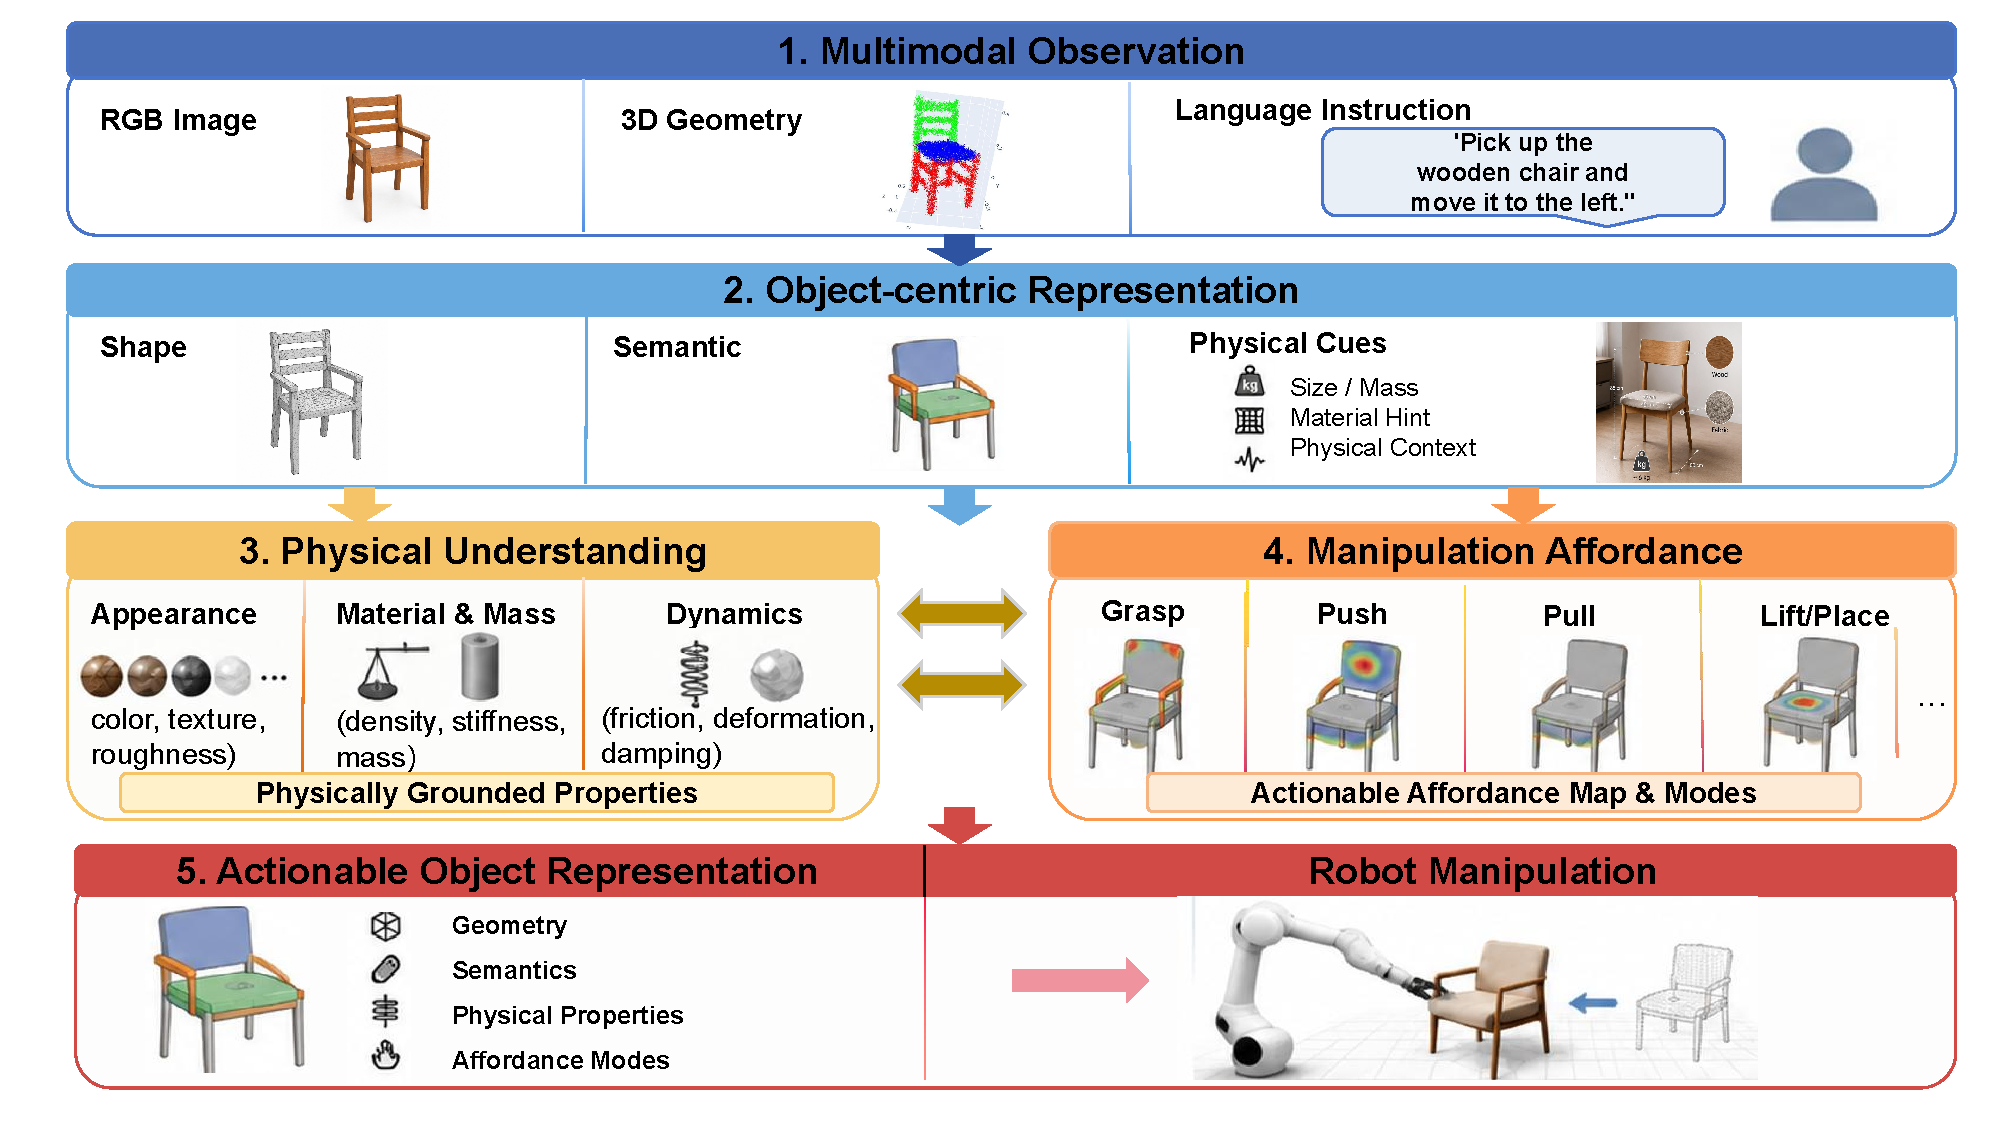
\includegraphics[width=0.98\textwidth]{Figures/fig4a.pdf}
%     \caption{Conceptual framework for physical‑functional indoor object understanding}
%     \label{fig:4a_concept}
% \end{figure}

% Semantic understanding provides object identities, spatial and semantic relations, and language-grounded descriptions, but these representations do not by themselves characterize how objects behave under physical interaction or which actions are feasible in a given context. Physical and functional understanding addresses this gap by connecting scene semantics with the physical properties, interaction possibilities, and state changes that govern embodied behavior.
% We organize this body of research into four complementary aspects:
% \emph{physical property estimation}, which infers material and mechanical attributes relevant to object behavior;
% \emph{affordance reasoning}, which identifies feasible interaction regions and action modes conditioned on the object, environment, and task;
% \emph{physical consequence prediction}, which anticipates how actions alter object and scene states; and
% \emph{physical consistency verification}, which evaluates whether reconstructed or predicted states satisfy geometric and physical constraints.
% These aspects are not strictly sequential: physical properties constrain affordances, affordances determine candidate actions, and physical prediction and verification assess the plausibility of their consequences. Together, they extend semantic-geometric scene understanding toward physically grounded and functionally meaningful representations, providing the information required for reliable action reasoning and planning.

% \subsection{Physical Property Estimation: Low-Level Parameters for Interaction Decisions}

% Physical properties are the low-level parameters of every interaction decision. Material, mass, and stiffness directly determine grasp force, motion trajectory, and stability judgment, and they provide the basis for the affordance and dynamics reasoning below. Surface materials (reflectance, roughness, transparency) and mechanical attributes (mass, rigidity, deformability) are both inferred from visual appearance. Knowing that a cup is glass immediately suggests fragility and calls for controlled grasp force, while a sofa is naturally expected to deform more than a wooden chair.
% Early material estimation relied on physically based rendering and illumination modeling. With neural rendering, deep networks now jointly reconstruct geometry and material, recovering reflectance and illumination parameters from complex scenes and laying the foundation for digital twins and photorealistic simulation~\cite{bi2020neural}. Mechanical property estimation further integrates visual cues with motion observations and physics-based simulation, so that, for example, a heavy cast-iron pan and a light plastic bowl are grasped with different forces and planned with different trajectories. Although humans perform such intuitive physical inference effortlessly, it remains challenging for vision systems, making dedicated estimation and benchmarking necessary.
% Material and mechanical estimation are increasingly treated as one problem, because both are read off the same visual observations and both feed the same downstream reasoning; the distinction is one of surface appearance versus bulk behavior, not of separate architectures.

% \begin{table}[!tbp]
% \centering
% \caption{Core perspectives and representative advances for physical and functional understanding in indoor scene understanding.}
% \label{tab:physical_functional_overview}
% \resizebox{\textwidth}{!}{
% \begin{tabular}{>{\centering\arraybackslash}p{4.2cm} |>{\centering\arraybackslash}p{7.0cm} |>{\centering\arraybackslash}p{7.4cm}}
% \rowcolor[RGB]{25,55,105}
% \textcolor{white}{\textbf{Core Perspective}}
% & \textcolor{white}{\textbf{Key Research Contents}}
% & \textcolor{white}{\textbf{Representative Strategies \& Works}} \\
% \hline
% \rowcolor[RGB]{220,230,245}
% \textbf{Physical Property Estimation}
% & Infer intrinsic object physical attributes (material, mechanical properties) from visual inputs; foundation-model-driven physical reasoning; simulation-ready physical 3D representation generation.
% & Neural Reflectance Fields~\cite{bi2020neural}; Physion benchmark~\cite{bear2021physion}; PhysBench~\cite{chow2025physbench}; QuantiPhy~\cite{li2025quantiphy}; PhysX-3D~\cite{cao2025physx3d} / PhysX-Anything~\cite{cao2025physxanything} \\
% \hline
% \textbf{Affordance Reasoning}
% & Reason about action possibilities enabled by objects; evolves from static geometric analysis toward demonstration-driven, interactive, and physically grounded affordance modeling.
% & AffordanceNet~\cite{do2018affordancenet}; Where2Act~\cite{mo2021where2act}; RAIL~\cite{zhang2024rail}; RoboPoint~\cite{yuan2024robopoint}; PhysXNet~\cite{cao2025physx3d} \\
% \hline
% \rowcolor[RGB]{220,230,245}
% \textbf{Physical Causal Reasoning}
% & Predict action-outcome transitions; temporal physical dynamics reasoning; counterfactual simulation for hypothetical physical scenarios.
% & CLEVRER~\cite{yi2019clevrer}; CausalVQA~\cite{foss2025causalvqa}; world-model-based counterfactual prediction frameworks~\cite{wang2026autonomous} \\
% \hline
% \textbf{Physical Consistency Verification}
% & Verify whether generated visual content or 3D assets obey physical laws; evaluate visual plausibility and executable simulation-ready physical consistency.
% & PhyGenBench~\cite{meng2024towards}; video world model analysis~\cite{brooks2024video,kang2024far}; PhysX-Anything~\cite{cao2025physxanything} \\
% \hline
% \rowcolor[RGB]{240,244,250}
% \multicolumn{3}{>{\centering\arraybackslash}p{18.6cm}}{\textbf{Overall Goal}: Build physically grounded unified representations including geometry, material, articulation, affordance and causal dynamics to support robotic manipulation, long-horizon planning and interactive world simulation.}
% \end{tabular}
% }
% \end{table}

% Beyond isolated attributes, foundation-model-era research evaluates comprehensive physical understanding. Physion provides one of the first systematic evaluations of physical interactions, covering support relations, collision dynamics, and object stability; it reveals that state-of-the-art vision models, despite impressive recognition performance, still fall considerably short of human-level physical reasoning~\cite{bear2021physion}. PhysBench scales this to a large benchmark covering mass, velocity, collision, and stability, testing whether foundation models have acquired fundamental knowledge of real-world physics~\cite{chow2025physbench}. QuantiPhy goes further by requiring quantitative predictions of numerical changes produced by physical processes rather than qualitative event recognition~\cite{li2025quantiphy}. Together these benchmarks show that the qualitative physical common sense of current vision and foundation models still lags behind humans, and that quantitative physical reasoning is not yet reliable enough to directly support fine-grained manipulation.
% The most embodiment-oriented direction constructs simulation-ready physical representations. PhysX-3D introduces the PhysXNet dataset, which annotates absolute scale, material, affordance, kinematics, and function at object and part levels, together with the PhysXGen dual-branch generation framework that jointly models geometric structure and physical properties, preserving geometric fidelity while maintaining physically plausible behavior~\cite{cao2025physx3d}. PhysX-Anything extends this to single in-the-wild images. A unified vision-language model jointly predicts geometry, articulation structures, physical attributes, and functional descriptions, and automatically exports standard URDF and XML files, so that generated assets can be deployed directly into physics simulators such as MuJoCo for manipulation and policy learning~\cite{cao2025physxanything}.
% Compared with geometry-oriented generation, such simulation-ready assets narrow the gap between visual perception and embodied interaction, integrating geometry, semantics, and physics into standardized forms that simulators can consume and downstream contact-rich policy learning can exploit. Physically grounded property estimation thus provides the low-level parameters on which all subsequent reasoning depends; the next layer asks what actions these properties make possible.
% These benchmarks also expose a modality gap: models that excel at recognition can fail on simple stability or collision judgments. This underscores that physical reasoning is not an emergent by-product of visual scale alone, and motivates combining perception with explicit physics priors. The dataset-level annotations of PhysXNet distinguish it from appearance-only 3D datasets, making it directly usable for training simulators and policies rather than only for rendering.
% Automated format conversion is the key enabler of simulation-ready generation: it removes the manual modeling bottleneck that previously separated perception from simulation, and lets a single image become an executable asset within minutes.

% \subsection{Affordance Reasoning: Judging Interaction Possibilities and Modes}

% Affordance reasoning directly answers ``where and how to operate'': it converts abstract physical properties into concrete interaction points and modes, and is the most direct bridge from semantics to action. According to Gibson's theory, every object offers potential actions: a chair affords sitting, a door affords pushing or pulling, a tabletop affords placing, and a drawer affords opening. Affordances therefore emphasize usability and action possibilities rather than mere category identity, and these functional properties provide essential knowledge for task execution.
% Early affordance research inferred functionality from geometry, assuming that shape determines use: horizontal surfaces afford placing, and container-like structures afford storage. AffordanceNet first jointly performed object detection and affordance segmentation in an end-to-end architecture, marking the shift from manual rules to data-driven affordance learning~\cite{do2018affordancenet}. Demonstration-based approaches instead learn affordances from human-object interactions, with large-scale first-person datasets such as EPIC-KITCHENS and Ego4D providing abundant manipulation examples from daily activities~\cite{damen2018scaling,grauman2022ego4d}. Both paradigms, however, rely on static shape or observed interactions, and generalize poorly to unseen objects and novel configurations.
% Interactive and physically grounded affordance reasoning has therefore become the core direction. Where2Act learns the mapping from action locations to interaction outcomes directly on point clouds, enabling robots to discover hidden affordances through active exploration of pushing, pulling, and grasping~\cite{mo2021where2act}. RAIL integrates language reasoning with physical simulation, generating candidate actions and verifying their feasibility under real-world constraints~\cite{zhang2024rail}. RoboPoint predicts manipulation points with vision-language models, unifying language, perception, and action spaces~\cite{yuan2024robopoint}. PhysXNet jointly annotates affordance with part-level material, kinematics, and function, so agents can reason not only where to interact but why the interaction is feasible under physical constraints~\cite{cao2025physx3d}.
% Taken together, affordance reasoning has evolved from static geometric analysis into a comprehensive framework integrating perception, language, and interaction experience, directly connecting the object instances of Chapter~IV to the operational decisions of Chapter~VI by turning physical properties into concrete interaction points and modes.
% Geometry-based methods are cheap and interpretable but fail when function depends on articulation, mechanism, or context rather than raw shape. Demonstration-based methods capture realistic usage but inherit the bias and coverage limits of the recorded activities. Affordance is thus not a property of the object alone but of the object-actor pair, which is why interaction-based methods are ultimately necessary.
% Interactive learning closes the loop by letting the robot probe the object and update its affordance model from the resulting state change, the paradigm most aligned with embodied exploration. The result is an affordance representation that is simultaneously language-addressable, geometry-grounded, and physics-verified.

% \begin{figure}[htbp]
%     \centering
%     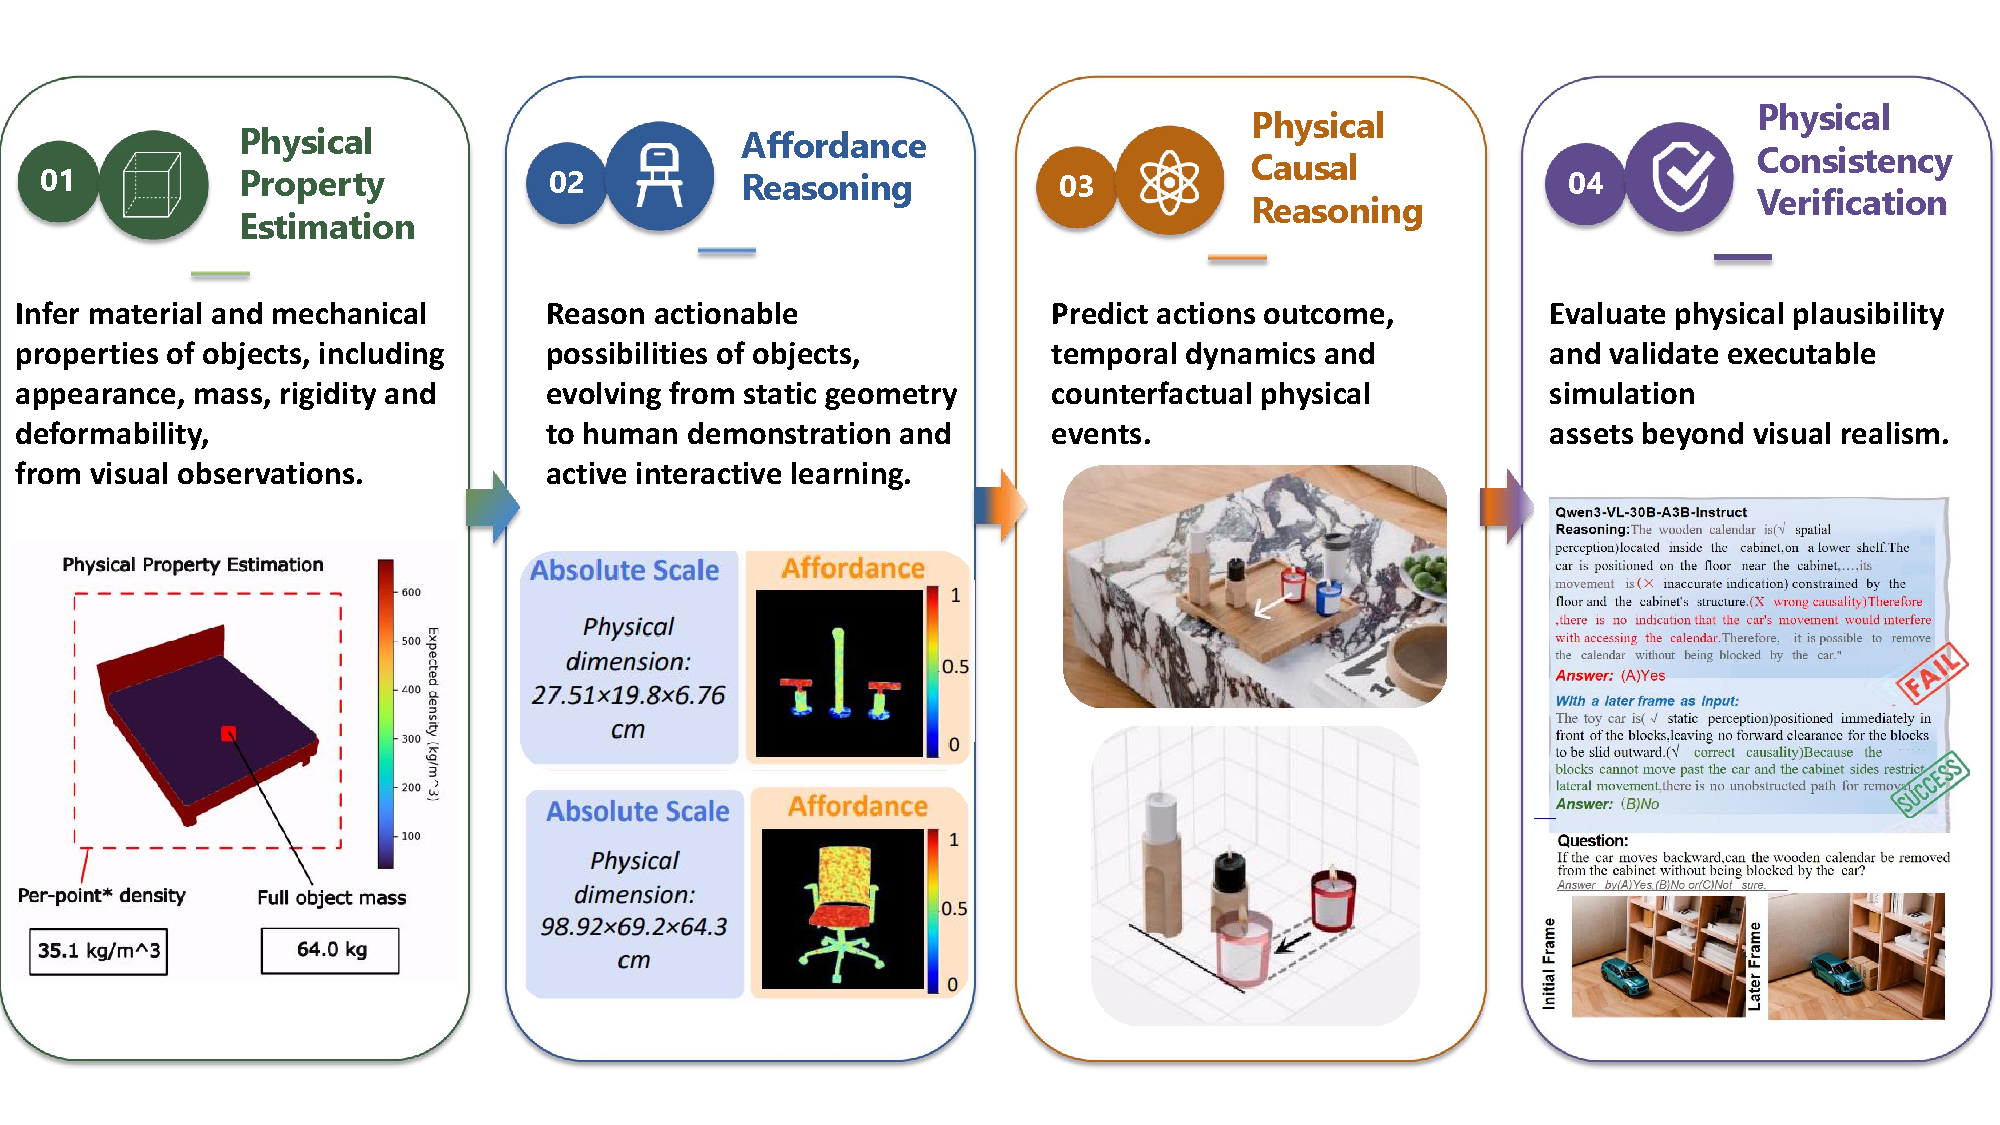
\includegraphics[width=0.98\textwidth]{Figures/fig4b.pdf}
%     \caption{Algorithm pipeline for generating simulation‑ready physical representations}
%     \label{fig:4b_pipeline}
% \end{figure}

% \subsection{Physical Causal Reasoning and Dynamics Prediction: Anticipating Interaction Consequences}

% Causal and dynamics prediction answer ``what happens after an action,'' upgrading the representation from ``what can be done'' to ``what happens once it is done.'' Actions inevitably alter environmental states: pushing a door opens it, grasping a cup changes its position, and pressing a switch turns on a light. Anticipating these transitions before execution is the core of long-horizon task planning and risk anticipation; for example, a safe plan must predict that excessive push force will slide the cup off the table before the motion is executed. This layer provides the physical dynamics basis for the world models and planning algorithms of Chapter~VI.
% Methodologically, action--outcome reasoning learns the mapping between actions and state transitions from video data, constructing action-effect models that predict future scene evolution and thereby support long-horizon planning. Temporal causal reasoning extends this to phenomena that unfold over time, such as pouring water gradually raising a liquid level. Benchmarks such as CLEVRER~\cite{yi2019clevrer} and CausalVQA~\cite{foss2025causalvqa} systematically evaluate why events occur and what happens next. Counterfactual reasoning goes further, asking what would have happened under alternative conditions: whether a door would still have opened without the push, or whether water would have spilled without the collision. This supports multi-plan comparison and risk pre-judgment before the agent commits to a decision. Recent world models increasingly incorporate such counterfactual simulation into unified predictive frameworks~\cite{wang2026autonomous}, foreshadowing the prediction-driven planning discussed in Chapter~VI.
% Because physical interactions are largely irreversible, the cost of wrong predictions is high, making foresight a prerequisite for safe autonomy. Action-effect models are typically learned from video, which provides dense supervision over states before and after each action. Synthetic benchmarks deliberately isolate physical causality from perceptual noise, although transferring their lessons to real scenes remains open. Counterfactual reasoning is also the mechanism behind ``what-if'' safety checks in manipulation planning, linking this section directly to the verification layer that follows.

% \subsection{Physical Consistency Verification: Closed-Loop Validation of Interaction Representation}

% Physical consistency verification is the final gate that moves a scene representation from ``looking plausible'' to ``being trustworthy for use.'' It checks that generated content obeys fundamental physical laws, such as gravity, collision, and occlusion: apples should fall downward, two solid objects cannot occupy the same space, and an occluded object preserves its identity. It also checks that 3D assets can be executed directly in simulators. This closes the perception-prediction-validation loop and provides the reliable substrate for the embodied policy learning discussed in Chapter~VI, reducing the operational failures caused by content that is visually plausible but physically wrong.
% Although these constraints are intuitive for humans, they remain difficult for generative models to learn reliably, and long-horizon physical consistency is a bottleneck even for recent video generative models with high visual fidelity. Dedicated benchmarks such as PhyGenBench evaluate physical commonsense in generated videos across gravity, collision, and support relationships~\cite{meng2024towards}. Analyses of large video world models further confirm substantial limitations in long-horizon causal reasoning and physical consistency, despite impressive visual quality~\cite{kang2024far}.
% The most embodiment-relevant direction is simulation-ready asset verification. PhysX-Anything evaluates whether generated assets, after automatic conversion to URDF/XML, can directly support contact-rich manipulation and policy learning in physics simulators~\cite{cao2025physxanything}, suggesting that future evaluation protocols should consider executable physical consistency in addition to visual realism.
% Overall, physical consistency verification is evolving from visual plausibility toward executable physical consistency, providing physically grounded representations for robotic manipulation, long-horizon planning, and interactive world simulation.
% Verification operates at two levels: semantic plausibility for generated media and executable consistency for simulation assets; it is also a key validation stage for simulation-to-real transfer. Violations are often sparse and subtle, such as objects floating slightly or penetrations lasting a few frames, so they are hard to capture with standard reconstruction losses. Physics-aware post-processing and differentiable simulation are increasingly used to enforce constraints during generation rather than only detecting violations afterward.
% This shifts the unit of evaluation from pixels to behaviors: an asset is good if a policy trained on it transfers, not merely if it looks realistic. Combined with the other layers of this chapter, verification completes a loop in which representations are generated, checked, and refined before deployment.

% This chapter has upgraded the representation from ``semantic description'' to ``action basis'' across physical properties, affordance reasoning, causal prediction, and consistency verification, completing the functional, physical, and consequence dimensions of an actionable scene representation. On this basis, Chapter~VI discusses how to realize the complete behavior loop from navigation to manipulation.

% ============================================================
% 4. Physical and Functional Understanding
% ============================================================

\section{Physical and Functional Understanding}
\label{sec:physical_functional}

Physical and functional understanding concerns how an object behaves and
what an agent can do with it, rather than only recognizing its category or
recovering its geometry. A scene representation may identify a drawer, a
bottle, or a chair, but this information alone does not specify whether the
object can be pushed, pulled, grasped, lifted, or placed. More importantly,
the feasibility of an action depends on the object state, contact location,
action direction, surrounding environment, and task.

As illustrated in Fig.~\ref{fig:4b_pipeline}, existing studies can be
organized into four closely related aspects: \emph{physical property
estimation}, \emph{affordance reasoning}, \emph{physical causal reasoning},
and \emph{physical consistency verification}. Physical property estimation
concerns attributes such as material, mass, stiffness, friction, and
deformability. Affordance reasoning determines which interactions are
possible under specific object, agent, and environmental conditions.
Physical causal reasoning considers how an action changes the state of a
scene and what consequences may follow. Physical consistency verification
checks whether reconstructed, predicted, or generated states satisfy relevant
geometric and physical constraints. Representative studies include PhysX-3D
for physics-grounded object properties and affordances~\cite{cao2025physx3d},
Where2Act for action-conditioned affordance prediction~\cite{mo2021where2act},
CLEVRER and CausalVQA for physical and causal reasoning
~\cite{yi2019clevrer,foss2025causalvqa}, and PhyGenBench for evaluating
physical consistency in generated videos~\cite{meng2024towards}.

\begin{figure}[!t]
    \centering
    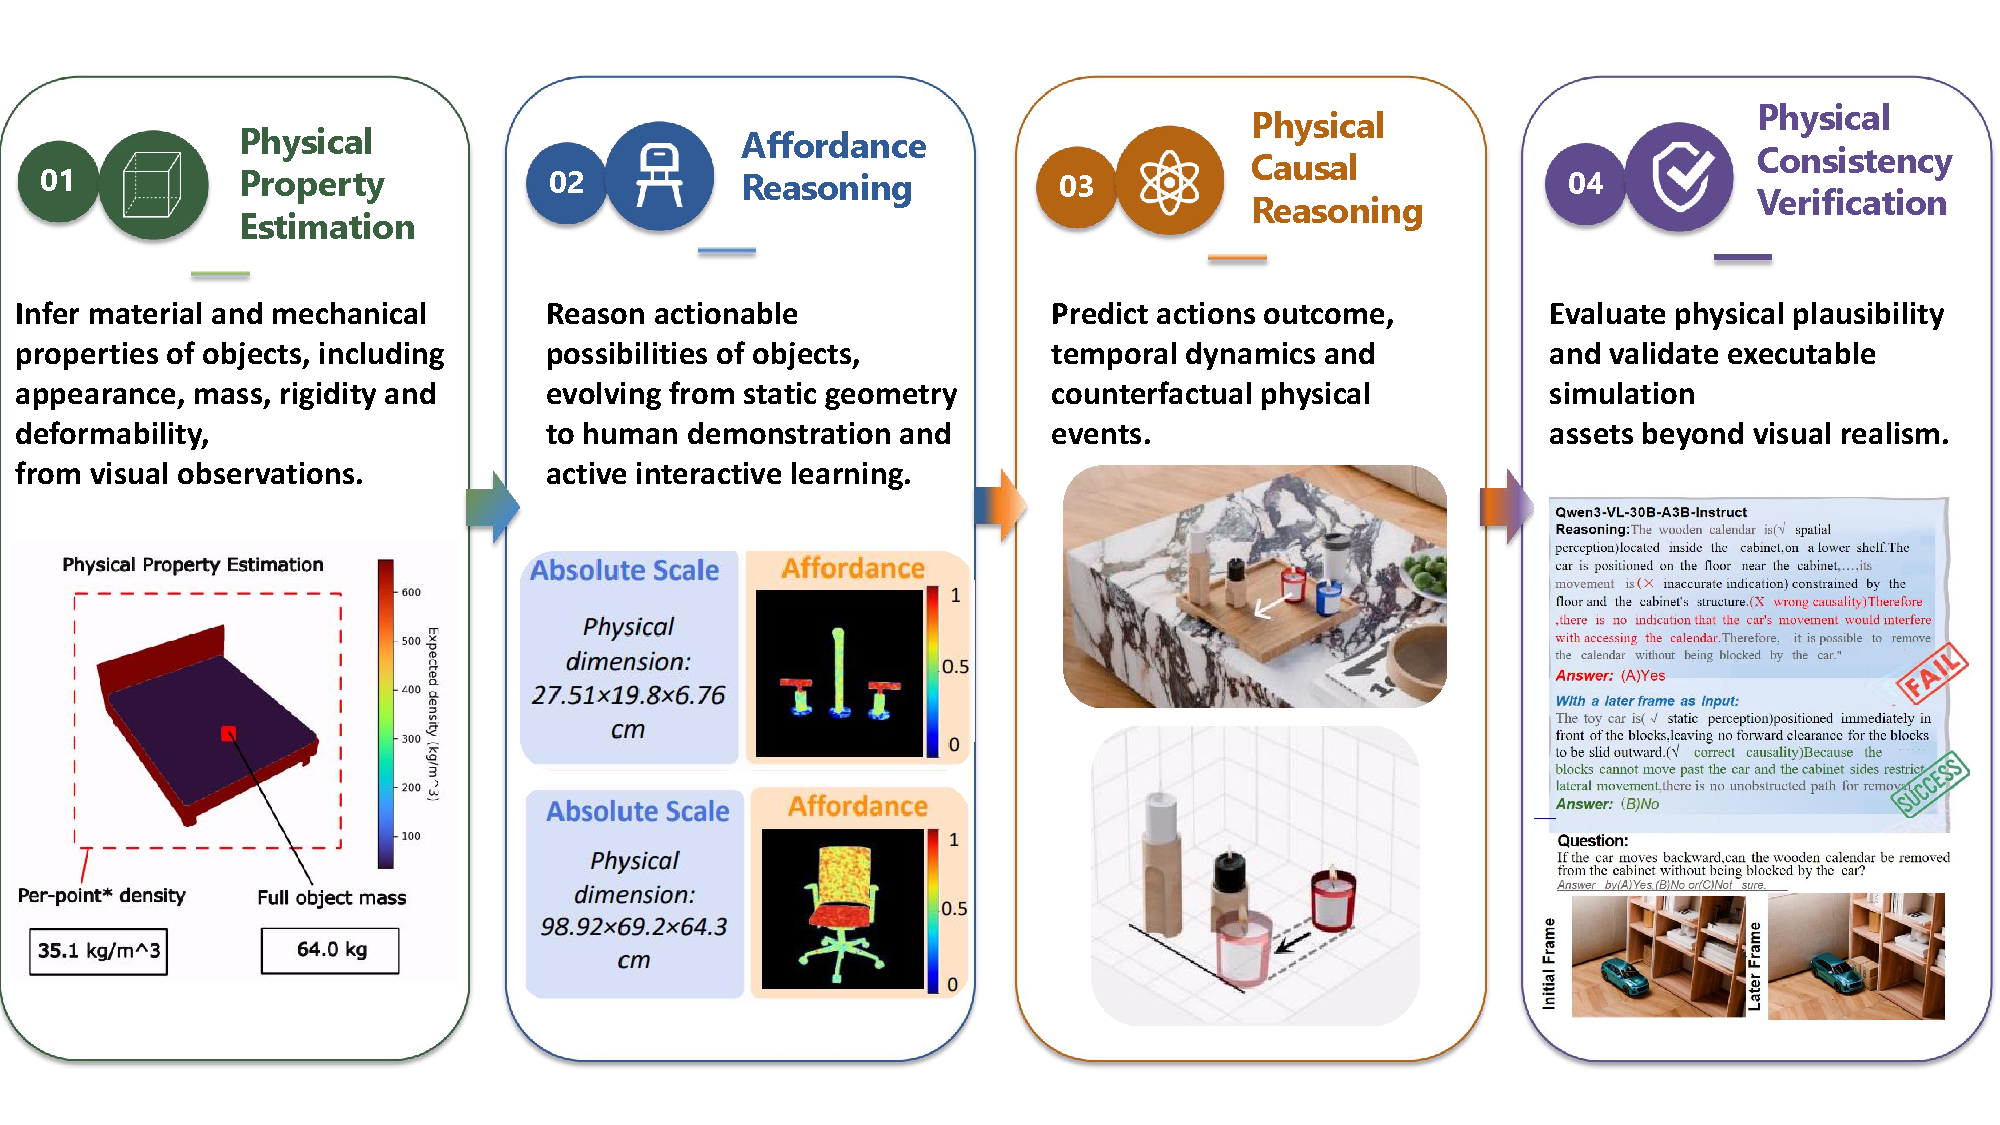
\includegraphics[width=\textwidth]{Figures/fig4b.pdf}
    \caption{Taxonomy of physical and functional understanding. Existing
    studies can be broadly organized into physical property estimation,
    affordance reasoning, physical causal reasoning, and physical consistency
    verification. Physical property estimation focuses on object attributes
    such as material, mass, rigidity, and deformability. Affordance reasoning
    identifies feasible interaction regions and action modes. Physical causal
    reasoning predicts action-induced changes, temporal dynamics, and
    counterfactual outcomes. Physical consistency verification evaluates
    whether reconstructed or generated states satisfy physical constraints
    and can support executable simulation. Representative studies include
    PhysX-3D~\cite{cao2025physx3d}, Where2Act~\cite{mo2021where2act},
    CLEVRER and CausalVQA~\cite{yi2019clevrer,foss2025causalvqa}, and
    PhyGenBench~\cite{meng2024towards}. The figure is a conceptual synthesis
    of these research directions.}
    \label{fig:4b_pipeline}
\end{figure}


% ============================================================
% 4.1 Physical Property Estimation
% ============================================================

\subsection{Physical Property Estimation}

Physical property estimation focuses on attributes that influence object
behavior but cannot be directly obtained from semantic labels. These
properties include both appearance-related characteristics, such as
reflectance and roughness, and mechanical characteristics, such as mass,
stiffness, friction, rigidity, and deformability. The distinction is
important for physical interaction because objects with similar appearance
or geometry can respond differently to the same action.

Traditional approaches mainly infer material or physical properties from
visual observations through inverse rendering or neural rendering. Such
methods establish a connection between image appearance and latent physical
attributes, but many mechanical properties are only weakly observable from
a single image. For example, the mass of two visually similar objects may
differ substantially, while stiffness and friction may have little direct
visual evidence.

Recent physics-grounded representations attempt to make these attributes
explicit. PhysX-3D incorporates absolute scale, material properties,
affordances, and kinematic information into a unified 3D representation
~\cite{cao2025physx3d}. Benchmarks such as PhysBench and QuantiPhy further
evaluate whether vision-language models can reason about physical properties
and their quantitative values rather than relying only on semantic
recognition~\cite{chow2025physbench,li2025quantiphy}.

The main issue is not simply whether a model can assign a physical label to
an object. What matters is whether the estimated property leads to a
reasonable prediction of object behavior. A mass estimate, for example,
becomes useful when it affects the predicted motion under an applied force.
Similarly, estimating rigidity or deformability is meaningful when the
property changes the predicted result of grasping or contact. This motivates
evaluating physical property estimation together with downstream prediction,
planning, and interaction rather than treating property recognition as an
independent classification task.


% ============================================================
% 4.2 Unified Physical Understanding and Affordance
% ============================================================

Physical properties alone do not determine how an object should be
manipulated. They must be considered together with geometry, object state,
task requirements, and environmental constraints. Fig.~\ref{fig:4a_concept}
summarizes this relationship, from multimodal observation and object-centric
representation to physical understanding, manipulation affordances, and
robot actions.

\begin{figure}[!t]
    \centering
    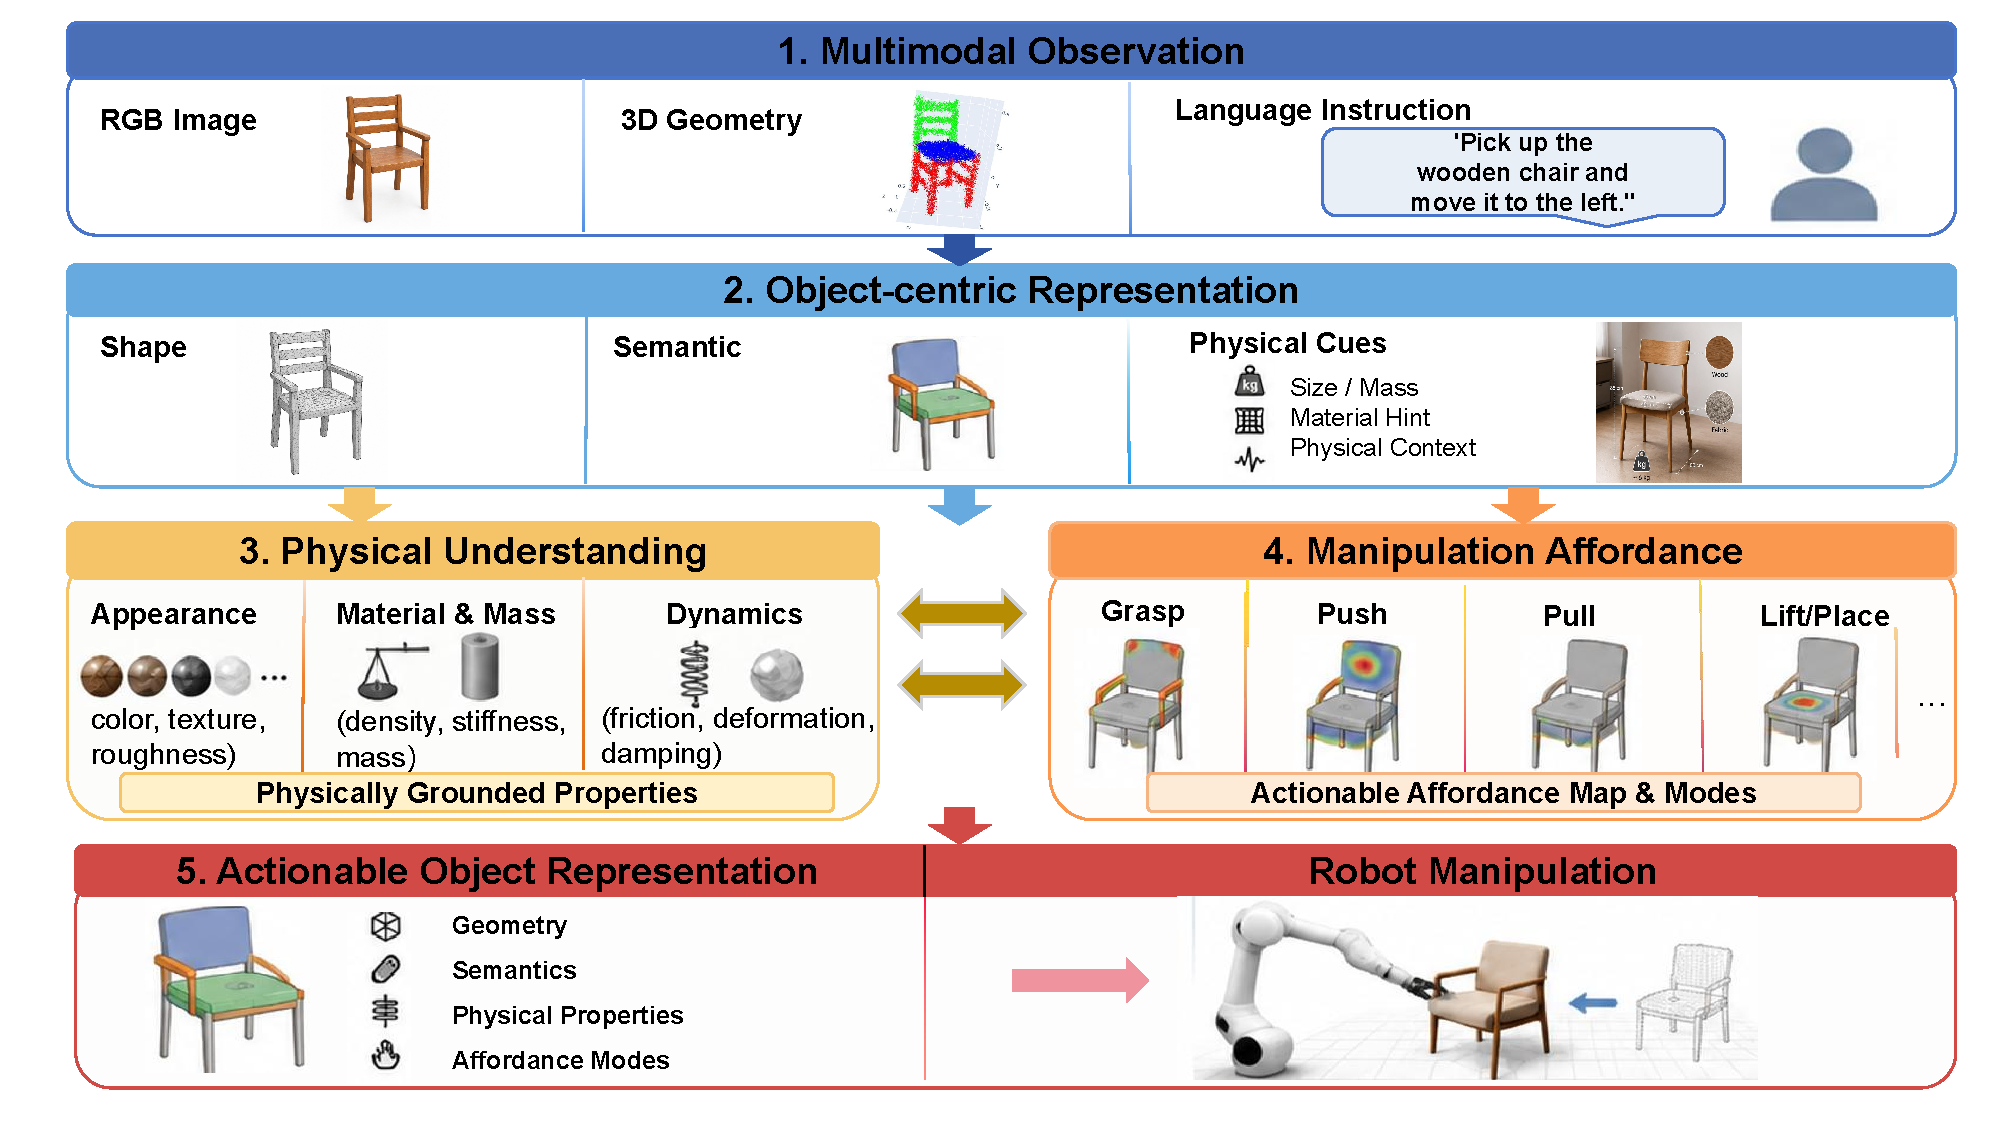
\includegraphics[width=\textwidth]{Figures/fig4a.pdf}
    \caption{From multimodal scene observation to physically grounded robot
    manipulation. Multimodal observations provide visual, geometric, and
    linguistic information, which is organized into object-centric
    representations containing geometry, semantics, and physical cues.
    Physical understanding estimates properties such as appearance, material,
    mass, and dynamics, while manipulation affordance associates these
    properties with feasible actions including grasping, pushing, pulling,
    lifting, and placing. The resulting actionable representation combines
    geometry, semantics, physical properties, and affordance modes for
    downstream robot manipulation. Representative formulations are discussed
    in PhysX-3D~\cite{cao2025physx3d}, Where2Act~\cite{mo2021where2act},
    RoboPoint~\cite{yuan2024robopoint}, and
    PhysX-Anything~\cite{cao2025physxanything}. The figure is a conceptual
    synthesis of these research directions.}
    \label{fig:4a_concept}
\end{figure}

The framework in Fig.~\ref{fig:4a_concept} highlights that physical
understanding is closely connected to action selection. RGB images, 3D
geometry, and language instructions provide different types of evidence
about an object and its context. These observations can be organized into
an object-centric representation containing semantic, geometric, and
physical information. Affordance reasoning then determines which
interactions are feasible under the current conditions. The resulting
actionable representation can be used by a robot to select and execute an
appropriate manipulation action.

This relationship is bidirectional. Physical properties constrain the set of
actions that can be safely executed, while candidate actions can also provide
information about uncertain physical properties. For example, whether a
drawer can be pulled depends not only on the presence of a handle, but also
on the drawer's current configuration, the available space behind the robot,
the direction of motion, and the interaction force. Thus, an affordance
should be represented as a relation between an object, an action, and the
conditions under which the action is feasible.


% ============================================================
% 4.3 Affordance Reasoning
% ============================================================

\subsection{Affordance Reasoning}

Affordance describes the possible interaction between an object and an
acting agent. A useful affordance representation should therefore answer
more than ``where can I interact?'' It should also describe ``what action
can be performed there?'', ``under what conditions can the action succeed?'',
and ``what state change will the action produce?'' This view treats
affordance as a \emph{conditional action-feasibility relation} rather than
as a static label attached to an object.

This distinction can be illustrated by a drawer. A static affordance label
may describe the drawer as ``pullable.'' However, successful pulling also
depends on whether the handle is reachable, whether the drawer is already
open, whether another object blocks its motion, and whether the robot has
sufficient space to apply the required force. The same drawer can therefore
have different feasible actions under different spatial configurations and
task conditions. Similar dependencies occur for pushing, grasping, lifting,
and placing.

Early affordance studies mainly focused on identifying functional regions
and action-related labels from visual observations. AffordanceNet introduced
an end-to-end framework for jointly detecting objects and their affordances
from RGB images, providing pixel-level affordance predictions
~\cite{do2018affordancenet}. Such formulations are useful for locating
interaction regions, but the predicted region alone does not determine
whether an action can be successfully executed in the current scene.

Where2Act further connects affordance prediction with action execution. It
predicts actionable regions on articulated 3D objects and generates
interaction trajectories for actions such as pushing and pulling
~\cite{mo2021where2act}. This formulation is closer to the actual
interaction problem because the output contains both an interaction location
and an associated action. RAIL incorporates language and physical
constraints when reasoning about functional regions and manipulation actions
~\cite{zhang2024rail}, while RoboPoint connects visual-language reasoning
with 3D point-based manipulation and task-specific interaction points
~\cite{yuan2024robopoint}. PhysX-3D further combines physical properties,
kinematics, and affordances within a physics-grounded 3D representation
~\cite{cao2025physx3d}.

These studies indicate a progression from \emph{affordance recognition} to
\emph{action-conditioned affordance reasoning}. The difference is important.
Recognition asks whether an object or region is associated with an action,
whereas reasoning requires the model to determine whether the action remains
feasible under the current conditions. In this setting, object geometry,
physical properties, task goals, and scene context jointly determine the
action space.

A further step is to connect affordance prediction with the expected
consequences of an action. An interaction point should not be considered
valid only because it is geometrically reachable. The resulting motion,
contact state, collision risk, and final object configuration also matter.
This creates a direct connection between affordance reasoning and physical
causal reasoning: affordance determines which actions are candidates, while
causal reasoning evaluates what may happen after those actions.


% ============================================================
% 4.4 Summary Table
% ============================================================

% ============================================================
% Colors
% ============================================================

\definecolor{TableHeader}{RGB}{45,55,72}
\definecolor{HeaderText}{RGB}{255,255,255}
\definecolor{LightBlue}{RGB}{239,246,255}
\definecolor{BorderGray}{RGB}{203,213,225}
\definecolor{TextGray}{RGB}{55,65,81}

\definecolor{PhysicalBlue}{RGB}{37,99,235}
\definecolor{AffordanceGreen}{RGB}{22,163,74}
\definecolor{CausalOrange}{RGB}{234,88,12}
\definecolor{ConsistencyPurple}{RGB}{126,34,206}

% ============================================================
% Column types
% ============================================================

\newcolumntype{L}[1]{
    >{\RaggedRight\arraybackslash}p{#1}
}

\newcolumntype{Y}{
    >{\RaggedRight\arraybackslash}X
}

% ============================================================
% Direction marker
% ============================================================

\newcommand{\researchdirection}[3]{%
    \textcolor{#1}{\large$\bullet$}\,
    \textbf{#2}
}

% ============================================================
% Table
% ============================================================

\begin{table}[t]
\centering

\caption{Representative research directions in physical and
functional understanding.}

\label{tab:physical_functional_overview}

\footnotesize
\renewcommand{\arraystretch}{1.45}
\setlength{\tabcolsep}{6pt}

\begin{tabularx}{\textwidth}{
    L{0.21\textwidth}
    L{0.45\textwidth}
    Y
}

% ------------------------------------------------------------
% Header
% ------------------------------------------------------------

\rowcolor{TableHeader}

\textcolor{HeaderText}{\textbf{Research Direction}}
&
\textcolor{HeaderText}{\textbf{Main Problem}}
&
\textcolor{HeaderText}{\textbf{Representative Works}}
\\

\midrule

% ------------------------------------------------------------
% Row 1
% ------------------------------------------------------------

\cellcolor{LightBlue}
\researchdirection{PhysicalBlue}
{Physical Property Estimation}
&
Estimate visual, material, and mechanical properties that
influence object behavior, including reflectance, roughness,
mass, stiffness, friction, and deformability.
&
Neural Reflectance Fields;
Physion~\cite{bear2021physion};
PhysBench~\cite{chow2025physbench};
QuantiPhy~\cite{li2025quantiphy};
PhysX-3D~\cite{cao2025physx3d};
PhysX-Anything~\cite{cao2025physxanything}
\\[4pt]

% ------------------------------------------------------------
% Row 2
% ------------------------------------------------------------

\cellcolor{LightBlue}
\researchdirection{AffordanceGreen}
{Affordance Reasoning}
&
Identify functional regions, feasible interaction modes,
and task-dependent actions for object manipulation.
&
AffordanceNet~\cite{do2018affordancenet};
Where2Act~\cite{mo2021where2act};
RAIL~\cite{zhang2024rail};
RoboPoint~\cite{yuan2024robopoint};
PhysX-3D~\cite{cao2025physx3d}
\\[4pt]

% ------------------------------------------------------------
% Row 3
% ------------------------------------------------------------

\cellcolor{LightBlue}
\researchdirection{CausalOrange}
{Physical Causal Reasoning}
&
Predict action-conditioned state transitions, temporal
dynamics, and counterfactual outcomes for physical
interaction and planning.
&
CLEVRER~\cite{yi2019clevrer};
CausalVQA~\cite{foss2025causalvqa};
world-model-based predictive frameworks
~\cite{wang2026autonomous}
\\[4pt]

% ------------------------------------------------------------
% Row 4
% ------------------------------------------------------------

\cellcolor{LightBlue}
\researchdirection{ConsistencyPurple}
{Physical Consistency Verification}
&
Evaluate whether reconstructed, predicted, or generated
states obey physical constraints and whether simulation
assets are executable.
&
PhyGenBench~\cite{meng2024towards};
video world-model analysis;
PhysX-Anything~\cite{cao2025physxanything}
\\
\bottomrule
\end{tabularx}
\end{table}


% ============================================================
% 4.5 Physical Causal Reasoning
% ============================================================

\subsection{Physical Causal Reasoning}

Physical causal reasoning concerns the relationship between an action and
the changes that follow in the scene. Given an initial state
$\mathcal{S}_t$, an action $a_t$, and a set of physical properties
$\mathcal{P}$, the future state can be expressed as

\begin{equation}
    \mathcal{S}_{t+1}
    =
    f(\mathcal{S}_t, a_t, \mathcal{P}),
\end{equation}

where $f$ represents the underlying physical transition. The transition may
involve object motion, contact formation, collision, support relations,
deformation, or changes in articulated configuration.

CLEVRER provides controlled video scenarios for reasoning about object
interactions and future events~\cite{yi2019clevrer}. The benchmark requires
models to distinguish observed events from possible future events and to
reason about object interactions over time. CausalVQA evaluates causal
reasoning about physical events and their consequences
~\cite{foss2025causalvqa}.

For embodied systems, causal reasoning is particularly relevant when
multiple actions are available. The model must not only predict what happens
next, but also compare possible outcomes under different actions. For
example, pushing an object toward an obstacle and pushing it away from the
obstacle may start from nearly identical visual observations but result in
different future states. Predicting these differences is important for
manipulation planning, collision avoidance, and action selection. Recent
predictive frameworks and world models explore this setting by modeling
possible future states under alternative actions~\cite{wang2026autonomous}.

The difficulty is that visually plausible predictions do not necessarily
satisfy physical laws. A generated trajectory may appear smooth while
violating contact constraints, gravity, or object dynamics. In addition,
synthetic benchmarks provide controlled environments that simplify
evaluation but do not capture all of the uncertainty found in real scenes.
For long-horizon interaction, prediction errors can also accumulate over
multiple steps. These limitations make short-horizon prediction, physical
constraints, and closed-loop feedback important for reliable causal
reasoning.


% ============================================================
% 4.6 Physical Consistency Verification
% ============================================================

\subsection{Physical Consistency Verification}

Physical consistency verification evaluates whether a reconstructed,
predicted, or generated scene state is physically plausible. Relevant
constraints depend on the task, but commonly include gravity, support,
contact, collision, non-penetration, articulation, and physically reasonable
object motion.

The need for physical verification becomes more apparent when generative
models are used for 3D reconstruction and video generation. A generated
scene can have realistic textures and visually plausible geometry while
still containing physically invalid events. An object may float without
support, penetrate another object during contact, or move in a direction
inconsistent with gravity. PhyGenBench evaluates physical commonsense in
generated videos through relations such as gravity, collision, and support
~\cite{meng2024towards}.

Physical verification can also be performed at the level of
simulation-oriented representations. PhysX-Anything focuses on generating
physical 3D assets with geometry, articulation, and physical attributes that
can be used in executable simulation~\cite{cao2025physxanything}. This
provides a stronger test than visual similarity alone because the estimated
representation must produce meaningful behavior when placed in a simulated
environment.

The distinction between visual and physical correctness is important. Two
reconstructed objects may have similar geometric errors while producing
different behavior under gravity or contact. Consequently, evaluation
should consider not only whether the reconstructed geometry looks correct,
but also whether the resulting object behaves correctly when subjected to
physical interaction. Simulation provides one practical way to perform such
tests, although simulated behavior remains an approximation of real-world
behavior because it depends on the physical model and parameter settings.


% ============================================================
% 4.7 Overall Discussion
% ============================================================

The four directions described above are closely connected. Physical property
estimation provides information about how an object may respond to external
forces. Affordance reasoning uses this information together with geometry,
task requirements, and scene context to determine feasible interactions.
Physical causal reasoning predicts the consequences of candidate actions,
while physical consistency verification checks whether the predicted or
generated state is physically valid.

This relationship suggests that affordance should not be treated as an
isolated classification problem. A label such as ``pull'' or ``grasp'' only
describes one part of an interaction. The actual affordance depends on where
the object is contacted, how the action is executed, what constraints are
present, and whether the resulting state is acceptable. In this sense,
affordance reasoning provides the connection between physical understanding
and action.

For example, consider a drawer. Its geometry may reveal a handle and its
semantic representation may identify the object as a drawer. However,
whether the drawer can actually be pulled depends on the handle's
accessibility, the drawer's current state, the available free space, and the
expected direction of motion. A physically grounded system should therefore
represent the drawer not simply as ``pullable,'' but as an object associated
with a set of conditional action possibilities. This formulation also
provides a natural interface between perception and robot planning.

The same principle applies to other manipulation actions. A grasp point is
useful only when the robot can reach it and the object can be stably grasped.
A pushing direction is useful only when the object can move along that
direction without unexpected collision. A placement action requires both a
valid target region and a physically stable final configuration. These
examples show why physical properties, affordances, causal prediction, and
physical verification should be considered together when evaluating
physically grounded scene understanding.


% ============================================================
% 4.8 Conclusion of the Section
% ============================================================

In summary, physical and functional understanding extends scene
understanding from object recognition and geometric reconstruction to object
properties, interaction possibilities, action consequences, and physical
validity. Physical property estimation, affordance reasoning, physical causal
reasoning, and physical consistency verification provide four complementary
views of this problem.

Among them, affordance reasoning plays an important connecting role. An
affordance is not merely a static label attached to an object; it describes
whether a particular action is feasible under specific physical, geometric,
task, and environmental conditions. This formulation connects object
properties with action selection and provides a natural transition from
scene understanding to robot manipulation. Future systems therefore need to
evaluate not only whether a model recognizes an affordance, but also whether
the predicted affordance leads to successful and physically consistent
interaction in realistic scenes.

% \section{Embodied Unified Modeling}
% The preceding sections progressively construct an actionable representation of the environment, from geometric structure to semantic meaning and physical-functional properties. Geometric reconstruction establishes the spatial substrate of the scene; semantic understanding associates this geometry with object identities, relations, and language-grounded meanings; and physical-functional understanding further characterizes the physical properties, affordances, and constraints that govern how objects can be interacted with. These representations should not be viewed as independent outputs, but as complementary layers of a common scene state that supports embodied behavior.

% Embodied unified modeling builds upon these representations to connect perception, reasoning, decision making, prediction, and action within a closed behavioral loop. The goal is not to replace geometric, semantic, or physical-functional understanding with a monolithic model, but to integrate these heterogeneous forms of scene knowledge so that they can be effectively grounded in embodied decision making and control. From this perspective, vision-language models provide broad semantic and linguistic reasoning; navigation models couple scene understanding with spatial decision making; vision-language-action models map multimodal observations and task goals to executable actions; and world or action models introduce prediction of future states and action consequences. These paradigms address complementary aspects of embodied intelligence and increasingly share representations, inputs, and outputs.

% Accordingly, this section organizes embodied unified modeling according to the progressive coupling of four capabilities: \emph{multimodal scene reasoning}, which interprets the reconstructed scene in semantic and linguistic context; \emph{spatial and task-level decision making}, which connects scene semantics, affordances, and task goals to navigation and manipulation decisions; \emph{action generation and control}, which transforms these decisions into executable behavior under physical constraints; and \emph{predictive modeling}, which anticipates future states and action consequences to support planning before execution. Emerging unified embodied models increasingly integrate these capabilities within shared architectures, while their reliability ultimately depends on the geometric, semantic, and physical-functional grounding established by the preceding representations.


% \begin{figure}[t]
% \centering
% 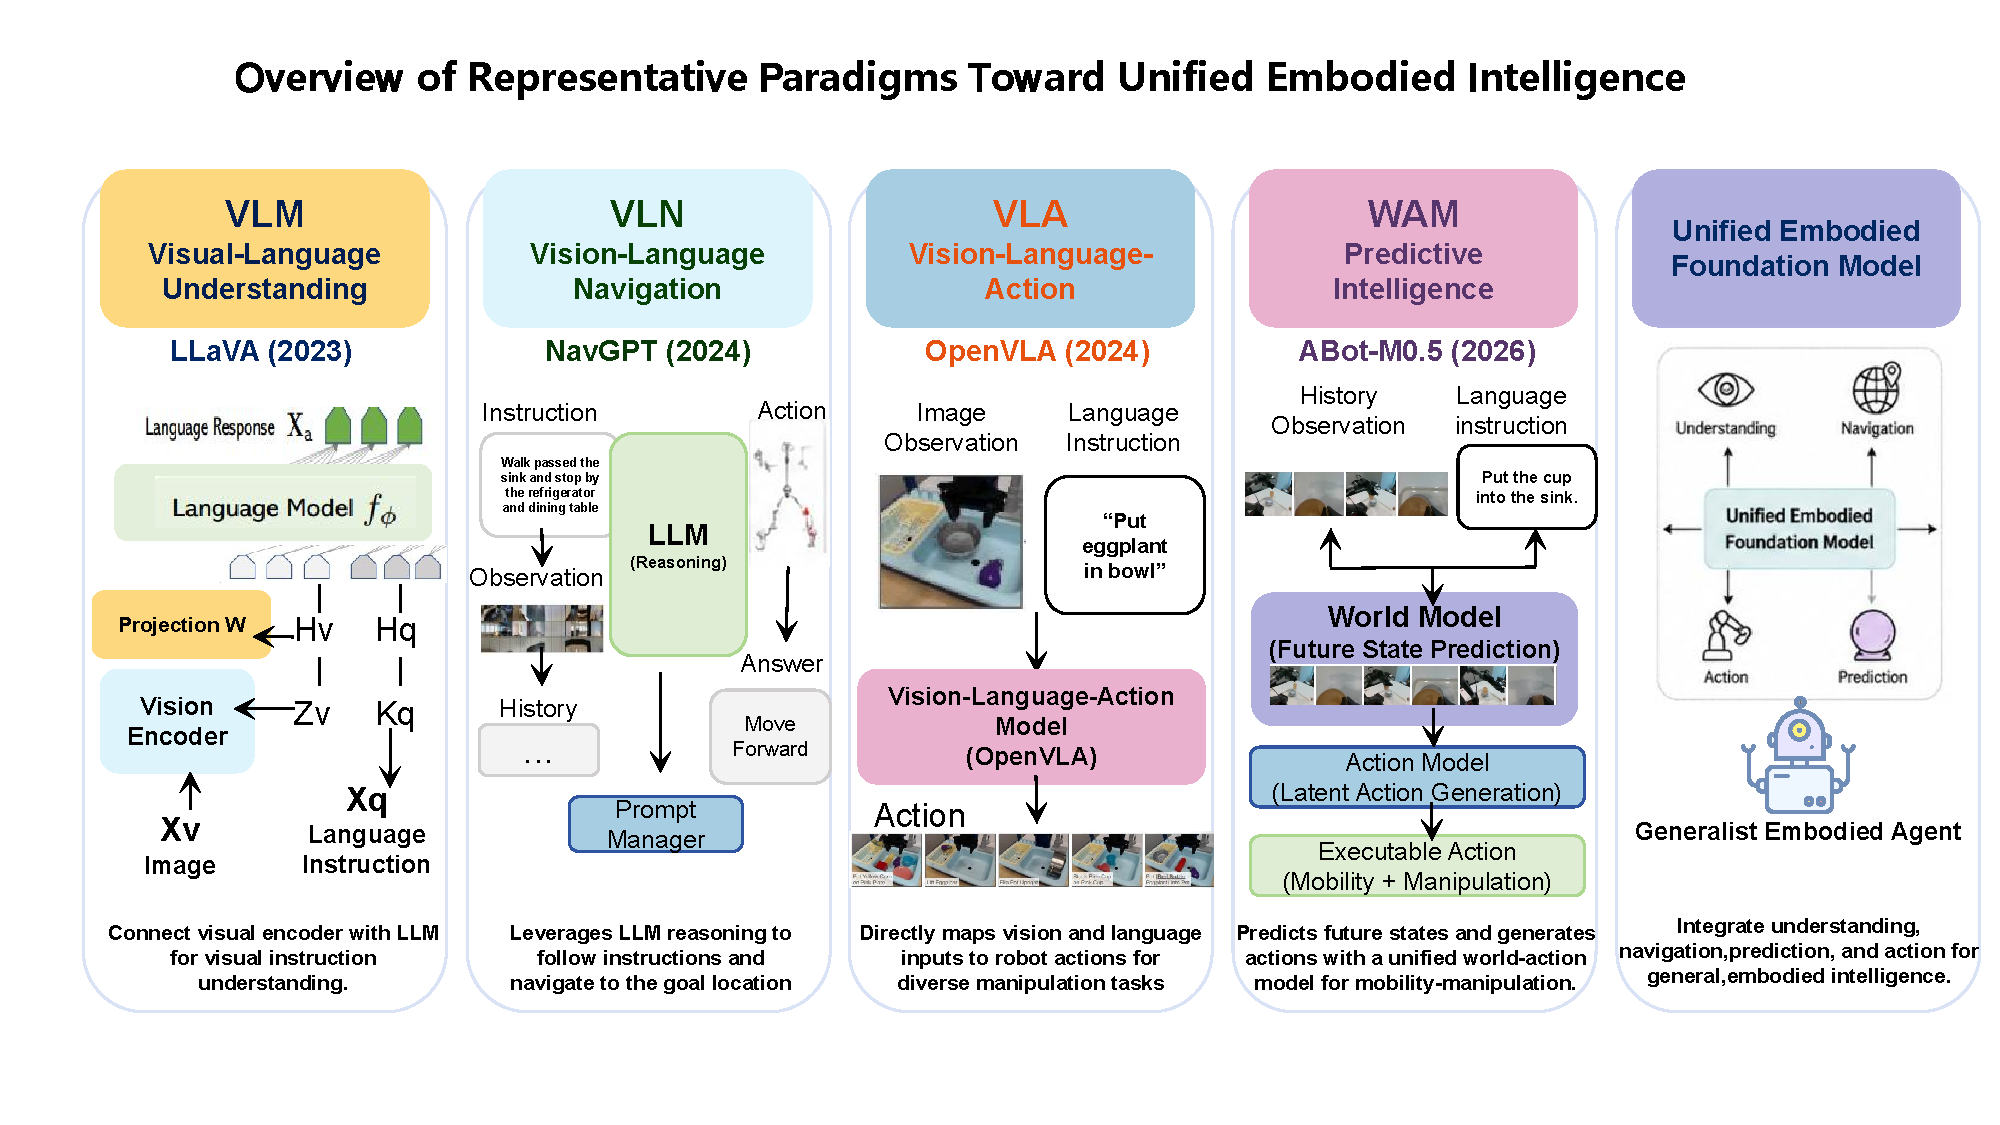
\includegraphics[width=0.96\textwidth]{Figures/Embodied Unified Modeling.pdf}
%  \caption{
%     Unified embodied modeling built upon geometric, semantic, and physical-functional scene representations. Rather than treating vision-language understanding, navigation, manipulation, and predictive modeling as independent stages, the framework progressively couples scene perception, semantic reasoning, physical grounding, future-state prediction, and action generation. Existing paradigms, including VLMs, VLN, VLA models, and world/action models, contribute complementary capabilities within this unified process, while emerging embodied foundation models increasingly integrate these capabilities into a shared modeling framework.
%     }
% \label{fig:embodied_unified_modeling}
% \end{figure}

% \begin{figure}[t]
% \centering
% 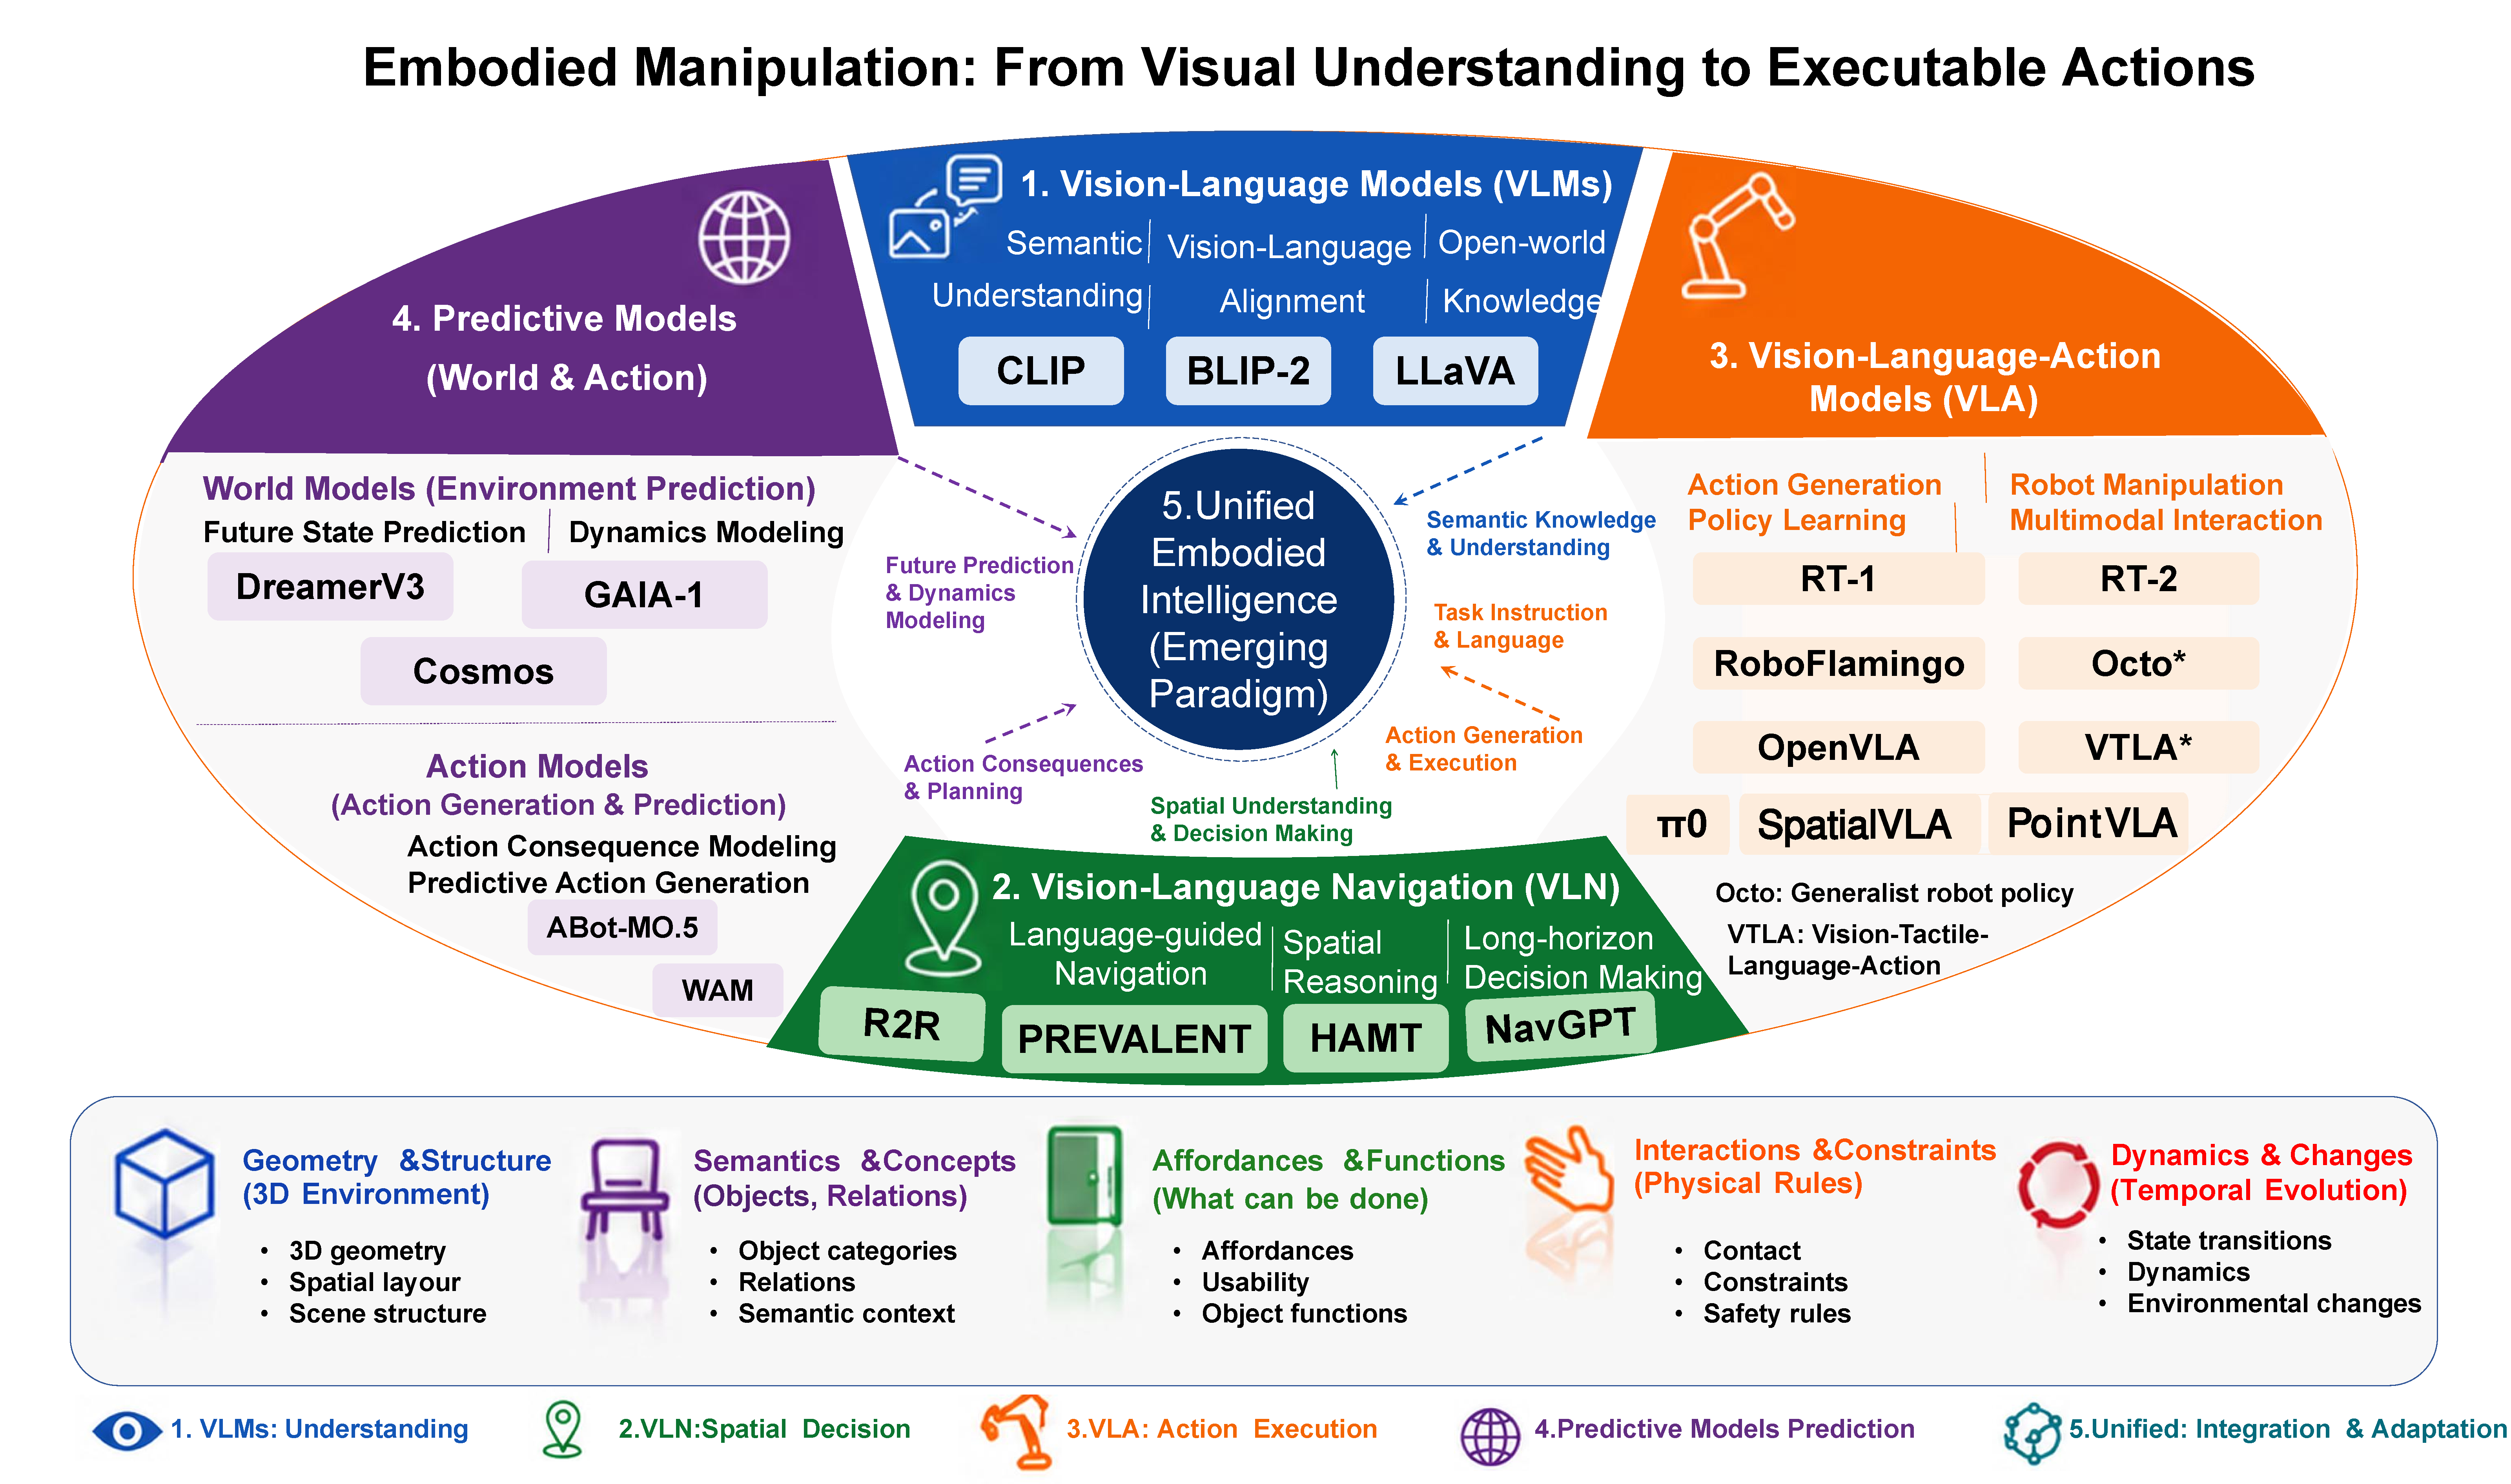
\includegraphics[width=0.96\textwidth]{Figures/fig_embodied_intelligence.pdf}
% \caption{
% Taxonomy of large-model-driven embodied intelligence from visual understanding to autonomous interaction. 
% The framework summarizes representative paradigms, including Vision-Language Models (VLMs), Vision-Language Navigation (VLN), Vision-Language-Action (VLA) models, world models and action models, and emerging unified embodied foundation models. 
% Rather than representing a strict sequential evolution, these paradigms provide complementary capabilities for semantic understanding, spatial reasoning, action generation, predictive modeling, and embodied interaction.
% }
% \label{fig:embodied_evolution}
% \end{figure}

% \subsection{Vision-Language Models: The Semantic Foundation for Embodied Interaction}

% VLMs provide the semantic interface layer of embodied intelligence. Through large-scale image-text pretraining, they supply open-world recognition, semantic association, and commonsense reasoning: contrastive alignment in CLIP connects visual concepts with natural language~\cite{radford2021clip}, and instruction tuning in BLIP-2 and LLaVA enables multimodal reasoning and complex visual instruction following~\cite{li2023blip,liu2023visual}. This turns the semantic units, scene graphs, and open-vocabulary understanding of Chapter~IV into a knowledge system that natural language can invoke, and it is the foundation of all instruction-driven tasks. For embodied agents this means more than recognizing objects: an agent must infer whether a chair can support sitting, whether it obstructs navigation, and how interacting with it affects surrounding objects.
% However, the semantic knowledge of VLMs does not directly translate into physical understanding: they are trained on image-text statistics rather than explicit models of geometry, dynamics, and physical constraints. VLMs therefore lack 3D spatial anchoring and interaction knowledge and cannot directly output actions; additional mechanisms are required to bridge visual-language understanding and reliable embodied action, motivating the navigation, manipulation, and prediction capabilities reviewed next.
% This language-grounded capability lets an agent interpret novel instructions without retraining, since words generalize beyond the exact phrases seen during pre-training. Closing the gap to action requires either grounding VLMs in 3D reconstruction or attaching physical readout modules that convert semantic beliefs into quantities usable for control; the following sections show how navigation, manipulation, and prediction each consume VLM semantics while adding the missing spatial or physical structure.

% \subsection{Vision-Language Navigation: Spatial-Semantics-Driven Mobility}

% VLN extends vision-language understanding to active spatial decision making: the agent receives natural-language instructions and visual observations and generates a sequence of navigation actions toward a target location. Navigation is essentially path planning in geometric space guided by semantic targets, so accurate reconstruction, room topology, and scene graphs are its core spatial basis; the Room-to-Room (R2R) benchmark established the standard indoor setting for this task~\cite{anderson2018vision}.
% Early VLN methods relied on sequence-based architectures that mapped observations and instructions directly to trajectories, but they generalized poorly because they lacked large-scale multimodal knowledge and struggled with long-horizon dependencies. The field has since progressed along three technical lines: vision-language pretraining that acquires transferable multimodal representations before task-specific training~\cite{hao2020towards}, Transformer-based historical trajectory modeling that better exploits previous observations during extended navigation~\cite{chen2021history}, and LLM-driven instruction reasoning and high-level planning~\cite{zhou2024navgpt}. Despite these advances, VLN remains limited by semantic-spatial alignment errors, long-horizon cumulative drift, and poor adaptation to dynamic environments; moreover, navigation is rarely an isolated objective, so future systems must integrate 3D scene understanding, affordance reasoning, and action planning.
% R2R and its successors also highlighted the central difficulty that instructions are underspecified, so agents must actively resolve ambiguity using visual context; long-horizon VLN additionally requires memory and replanning because perceptual aliasing and partial observability accumulate over long trajectories. A promising direction is to couple VLN with the scene graph and layout representations of Chapter~IV, turning navigation into graph search over a maintained topological map.

% \subsection{Vision-Language-Action Models: Mapping Multimodal Perception to Manipulation}

% VLA models are the core execution module of embodied manipulation: they map multimodal perception and language instructions directly to robot control commands, taking an object's semantics, location, and interaction mode as input and outputting executable behaviors. This level corresponds to the joint use of the semantic and physical-functional representations of Chapters~IV and V: the affordance and physical properties of an object determine whether the generated action is reasonable, so VLA models provide a unified interface between foundation models and robotic control.
% RT-1 introduced a Transformer-based robot policy trained on diverse real-world demonstrations and showed that scaling robot data improves generalization across manipulation tasks~\cite{brohan2022rt}; RT-2 further transferred web-scale vision-language knowledge into robotic control, demonstrating that pretrained multimodal representations provide useful semantic priors for manipulation~\cite{zitkovich2023rt}. RoboFlamingo showed that such representations can be adapted without training visual understanding from scratch, though its performance remains sensitive to demonstration quality~\cite{li2024vision}. Open-source generalist policies such as Octo and OpenVLA then advanced large-scale cross-task and cross-embodiment training, providing reusable foundations for adapting policies to downstream tasks while depending on the availability and diversity of robot interaction data~\cite{team2024octo,kim2024openvla}.
% Recent extensions enrich the paradigm with additional signals and mechanisms. VTLA integrates tactile information with visual and linguistic inputs for contact-rich manipulation, addressing interactions that cannot be fully inferred from appearance alone~\cite{zhang2026vtla}; DyPES-VLA incorporates dynamics priors into vision-language-action learning, shifting from purely reactive action generation toward predictive decision making~\cite{li2026dypesvla}; and $\pi_0$ proposes a vision-language-action flow model that represents complex, continuous action distributions across tasks and embodiments, providing greater flexibility than discrete action prediction~\cite{team2024pi0}.
% Nevertheless, current VLA systems remain dominated by imitation learning: they learn correlations between observations and actions rather than explicitly reasoning about the physical consequences of actions, and their generalization depends heavily on the availability and diversity of demonstration data. These limitations in long-horizon reasoning and safety-critical execution motivate the prediction-driven models of the next section.
% Unlike VLMs that interpret and VLN that move, VLA models must commit to concrete motor commands, so they are the point at which representational quality directly meets physical reality. The early results also established two empirical findings that shaped the field: data scale matters more than architecture for generalization, and vision-language pretraining transfers to control; at the same time, high-quality demonstration data remains expensive, motivating simulation and teleoperation pipelines.
% Sensory and generative extensions are motivated by the same limitation: appearance alone cannot disambiguate weight, friction, or compliance, all of which determine successful contact, and generative formulations admit multiple plausible actions for the same observation, which is closer to the true distribution of human behavior than a single deterministic output. As a result, VLA policies degrade gracefully on familiar tasks but fail predictably on novel dynamics, and they cannot simulate the consequences of their own actions; these gaps reflect the absence of an internal predictive model, which is exactly what world models provide.

% \subsection{World Models and Action Models: Prediction-Driven Planning and Decision Making}

% World models and action models together form a prediction-driven planning module. World models address the reactive limitation of VLA policies by learning internal representations of environmental dynamics and predicting possible future states, while action models emphasize how an agent should behave under specific conditions by connecting environmental states, task objectives, and executable behaviors; their fusion yields world action models (WAMs) that link future-state forecasting with robot control. Prediction upgrades the agent from a ``see-then-react'' reactive policy to an ``anticipate-then-plan'' proactive decision maker, enabling risk avoidance and multi-plan comparison before execution; this internalizes Chapter~V's causal reasoning as the agent's predictive simulator.
% Representative efforts span latent-dynamics world models that demonstrate scalable learning and efficient behavior generation across diverse environments~\cite{hafner2023mastering}, generative world modeling at scale for realistic physical scenarios, from driving environments to interactive video worlds~\cite{hu2023gaia,bruce2024genie}, and unified mobility-and-manipulation world action models that jointly model navigation and manipulation rather than treating them as independent problems~\cite{chen2026abot}. These studies suggest that predictive modeling can support embodied reasoning by letting agents consider possible future states before acting.
% However, generating plausible future observations does not imply genuine physical understanding: a model may produce visually realistic predictions while failing to capture object dynamics, contact relationships, or long-term consequences. World models and action models therefore remain at an early stage for real-world embodied applications: they require richer interaction data than static demonstrations because learning action consequences depends on diverse experiences, and long-horizon prediction suffers from partial observability, complex object interactions, and environmental uncertainty. They should be viewed as complementary to, rather than replacements for, VLA systems, providing the missing ability to anticipate future states and reason about action consequences.
% World models originate from reinforcement learning, where compact latent representations of environments support planning and imagination-based behavior; the structural difference from VLA is that the loop becomes observation-to-state prediction and state-conditioned action selection rather than direct observation-to-action mapping. Latent-dynamics models learn in compressed state spaces, making long-horizon imagination computationally tractable, whereas video-level generative models prioritize visual fidelity at higher cost.
% ABot-M0.5 is notable for treating mobility and manipulation as one predictive problem, so that a single model can decide whether to navigate, reach, or rearrange; GAIA-1 and Genie illustrate the same spectrum from structured driving scenes to open-ended controllable video, both treating prediction as generation. The data requirements of predictive models also differ: action consequences must be observed under diverse conditions, which static demonstration sets cannot provide, and evaluation often reduces to reconstruction quality rather than decision quality. Whether predictions are physically faithful enough to plan against remains an open question that connects directly to the consistency verification of Chapter~V.

% \begin{table}[!tbp]
% \centering

% \caption{
% Taxonomy of Embodied Intelligence: From Visual Understanding to Executable Actions
% }

% \label{tab:embodied_taxonomy}

% \renewcommand{\arraystretch}{1.35}

% \rowcolors{2}{gray!10}{white}

% \begin{tabularx}{\textwidth}{
% >{\centering\arraybackslash}p{2.7cm}
% >{\centering\arraybackslash}p{2.7cm}
% >{\centering\arraybackslash}p{4.0cm}
% >{\centering\arraybackslash}X
% >{\centering\arraybackslash}X
% }

% \toprule

% \rowcolor{blue!70}

% \textcolor{white}{\textbf{Paradigm}}
% &
% \textcolor{white}{\textbf{Core Objective}}
% &
% \textcolor{white}{\textbf{Representative Works}}
% &
% \textcolor{white}{\textbf{Main Capabilities}}
% &
% \textcolor{white}{\textbf{Remaining Challenges}}
% \\

% \midrule

% \textbf{Vision-Language Models (VLMs)}
% &
% Semantic understanding
% &
% CLIP ~\cite{radford2021clip}, 
% BLIP-2 ~\cite{li2023blip}, 
% LLaVA ~\cite{liu2023visual}
% &
% Vision-language alignment, open-world recognition, multimodal reasoning, semantic knowledge transfer
% &
% Limited 3D grounding, weak physical understanding, and insufficient interaction reasoning
% \\

% \textbf{Vision-Language Navigation (VLN)}
% &
% Language-guided spatial decision making
% &
% R2R ~\cite{anderson2018vision}, 
% PREVALENT ~\cite{hao2020towards}, 
% HAMT ~\cite{chen2021history}, 
% NavGPT ~\cite{zhou2024navgpt}
% &
% Instruction following, spatial reasoning, historical trajectory modeling, and long-horizon navigation
% &
% Ambiguous instructions, accumulated navigation errors, incomplete observations, and adaptation to dynamic environments
% \\

% \textbf{Vision-Language-Action (VLA) Models}
% &
% Multimodal perception-to-action mapping
% &
% RT-1 ~\cite{brohan2022rt}, 
% RT-2 ~\cite{zitkovich2023rt}, 
% RoboFlamingo ~\cite{li2024vision}, 
% Octo ~\cite{team2024octo}, 
% OpenVLA ~\cite{kim2024openvla}, 
% VTLA ~\cite{zhang2026vtla}
% &
% Robot action generation, imitation learning, task generalization, cross-embodiment transfer, and multimodal physical interaction
% &
% High cost of robot data, distribution shift, limited physical reasoning, and unreliable long-horizon execution
% \\

% \textbf{World and Action Models}
% &
% Predicting environmental evolution and action consequences
% &
% World Models ~\cite{ha2018world}, 
% DreamerV3 ~\cite{hafner2023mastering}, 
% GAIA-1 ~\cite{hu2023gaia}, 
% Genie ~\cite{bruce2024genie}, 
% ABot-M0.5 ~\cite{chen2026abot}
% &
% Latent dynamics modeling, future-state prediction, imagination-based planning, action-conditioned prediction, and mobility-manipulation coordination
% &
% Long-horizon prediction accuracy, physical consistency, action grounding, and real-world robustness
% \\

% \midrule

% \textbf{Unified Embodied Intelligence}
% &
% Cross-paradigm integration
% &
% Emerging integration of multimodal understanding, action generation, and predictive modeling
% &
% Joint use of semantic reasoning, spatial understanding, physical interaction, environmental prediction, and feedback
% &
% No established unified architecture, high data and computation requirements, safety, and generalization in open environments
% \\

% \bottomrule

% \end{tabularx}

% \end{table}

% \subsection{Unified Embodied Foundation Models: Toward Generalist Embodied Agents}

% Unified embodied foundation models aim to integrate multimodal understanding, spatial reasoning, predictive modeling, and action generation within a shared framework, moving the actionable scene representation from hierarchical construction toward unified fusion. Early steps include injecting 3D scene understanding into VLA frameworks (3D-VLA), which incorporates spatial reasoning and generative modeling so that scene structures constrain action generation~\cite{zhen20243d}, and physical-world foundation models such as Cosmos that provide general representations for Physical AI, which serves as useful supporting infrastructure rather than complete robotic intelligence, since reliable action also requires task reasoning, control, and continuous interaction with the environment.
% Despite these advances, unified models remain at an early stage: physical grounding is insufficient, interaction data are costly, and generalization to open environments is difficult; these are precisely the core bottlenecks that the scene representation must overcome to move from ``perceivable'' to ``executable.'' Unlike digital tasks, embodied agents operate under physical constraints where inaccurate predictions can lead to irreversible failures, so physical grounding and causal understanding cannot be replaced by simply scaling parameters or multimodal data. Evaluation is equally challenging: existing benchmarks focus on short-horizon tasks and predefined environments, so they cannot fully measure reasoning ability, robustness, safety, and adaptation efficiency.
% Overall, unified embodied foundation models provide a potential pathway toward integrating perception, reasoning, prediction, and action, but achieving general-purpose embodied agents still requires stronger physical grounding, predictive world modeling, efficient robot data utilization, and closed-loop interaction with the physical world.
% A shared representation is intended to let one experience benefit many tasks: language understanding improves manipulation, prediction improves navigation, and so on; 3D-VLA is representative of the trend to make action generation explicitly conditioned on geometry rather than flat image tokens, and Cosmos is best understood as the perceptual-physical substrate on which more specialized task models are built.
% Data and computation costs also grow superlinearly with the number of integrated capabilities, and safety is a further concern because an integrated model concentrates risk: perception failures propagate to planning and control unless architectures provide isolation or verification. Benchmarks must therefore be redesigned around long-horizon, open-world tasks that jointly exercise perception, reasoning, prediction, and control.

% This chapter has completed the transformation from scene representation to embodied action across semantic understanding, navigation, manipulation, predictive planning, and unified integration. The current representation and modeling system, however, still concentrates on visible, static, and task-oriented scenes; Chapter~VII summarizes the core challenges and proposes future research directions.
\section{Executable Embodied Manipulation}
\label{sec:executable_manipulation}
\begin{figure}[t]
\centering
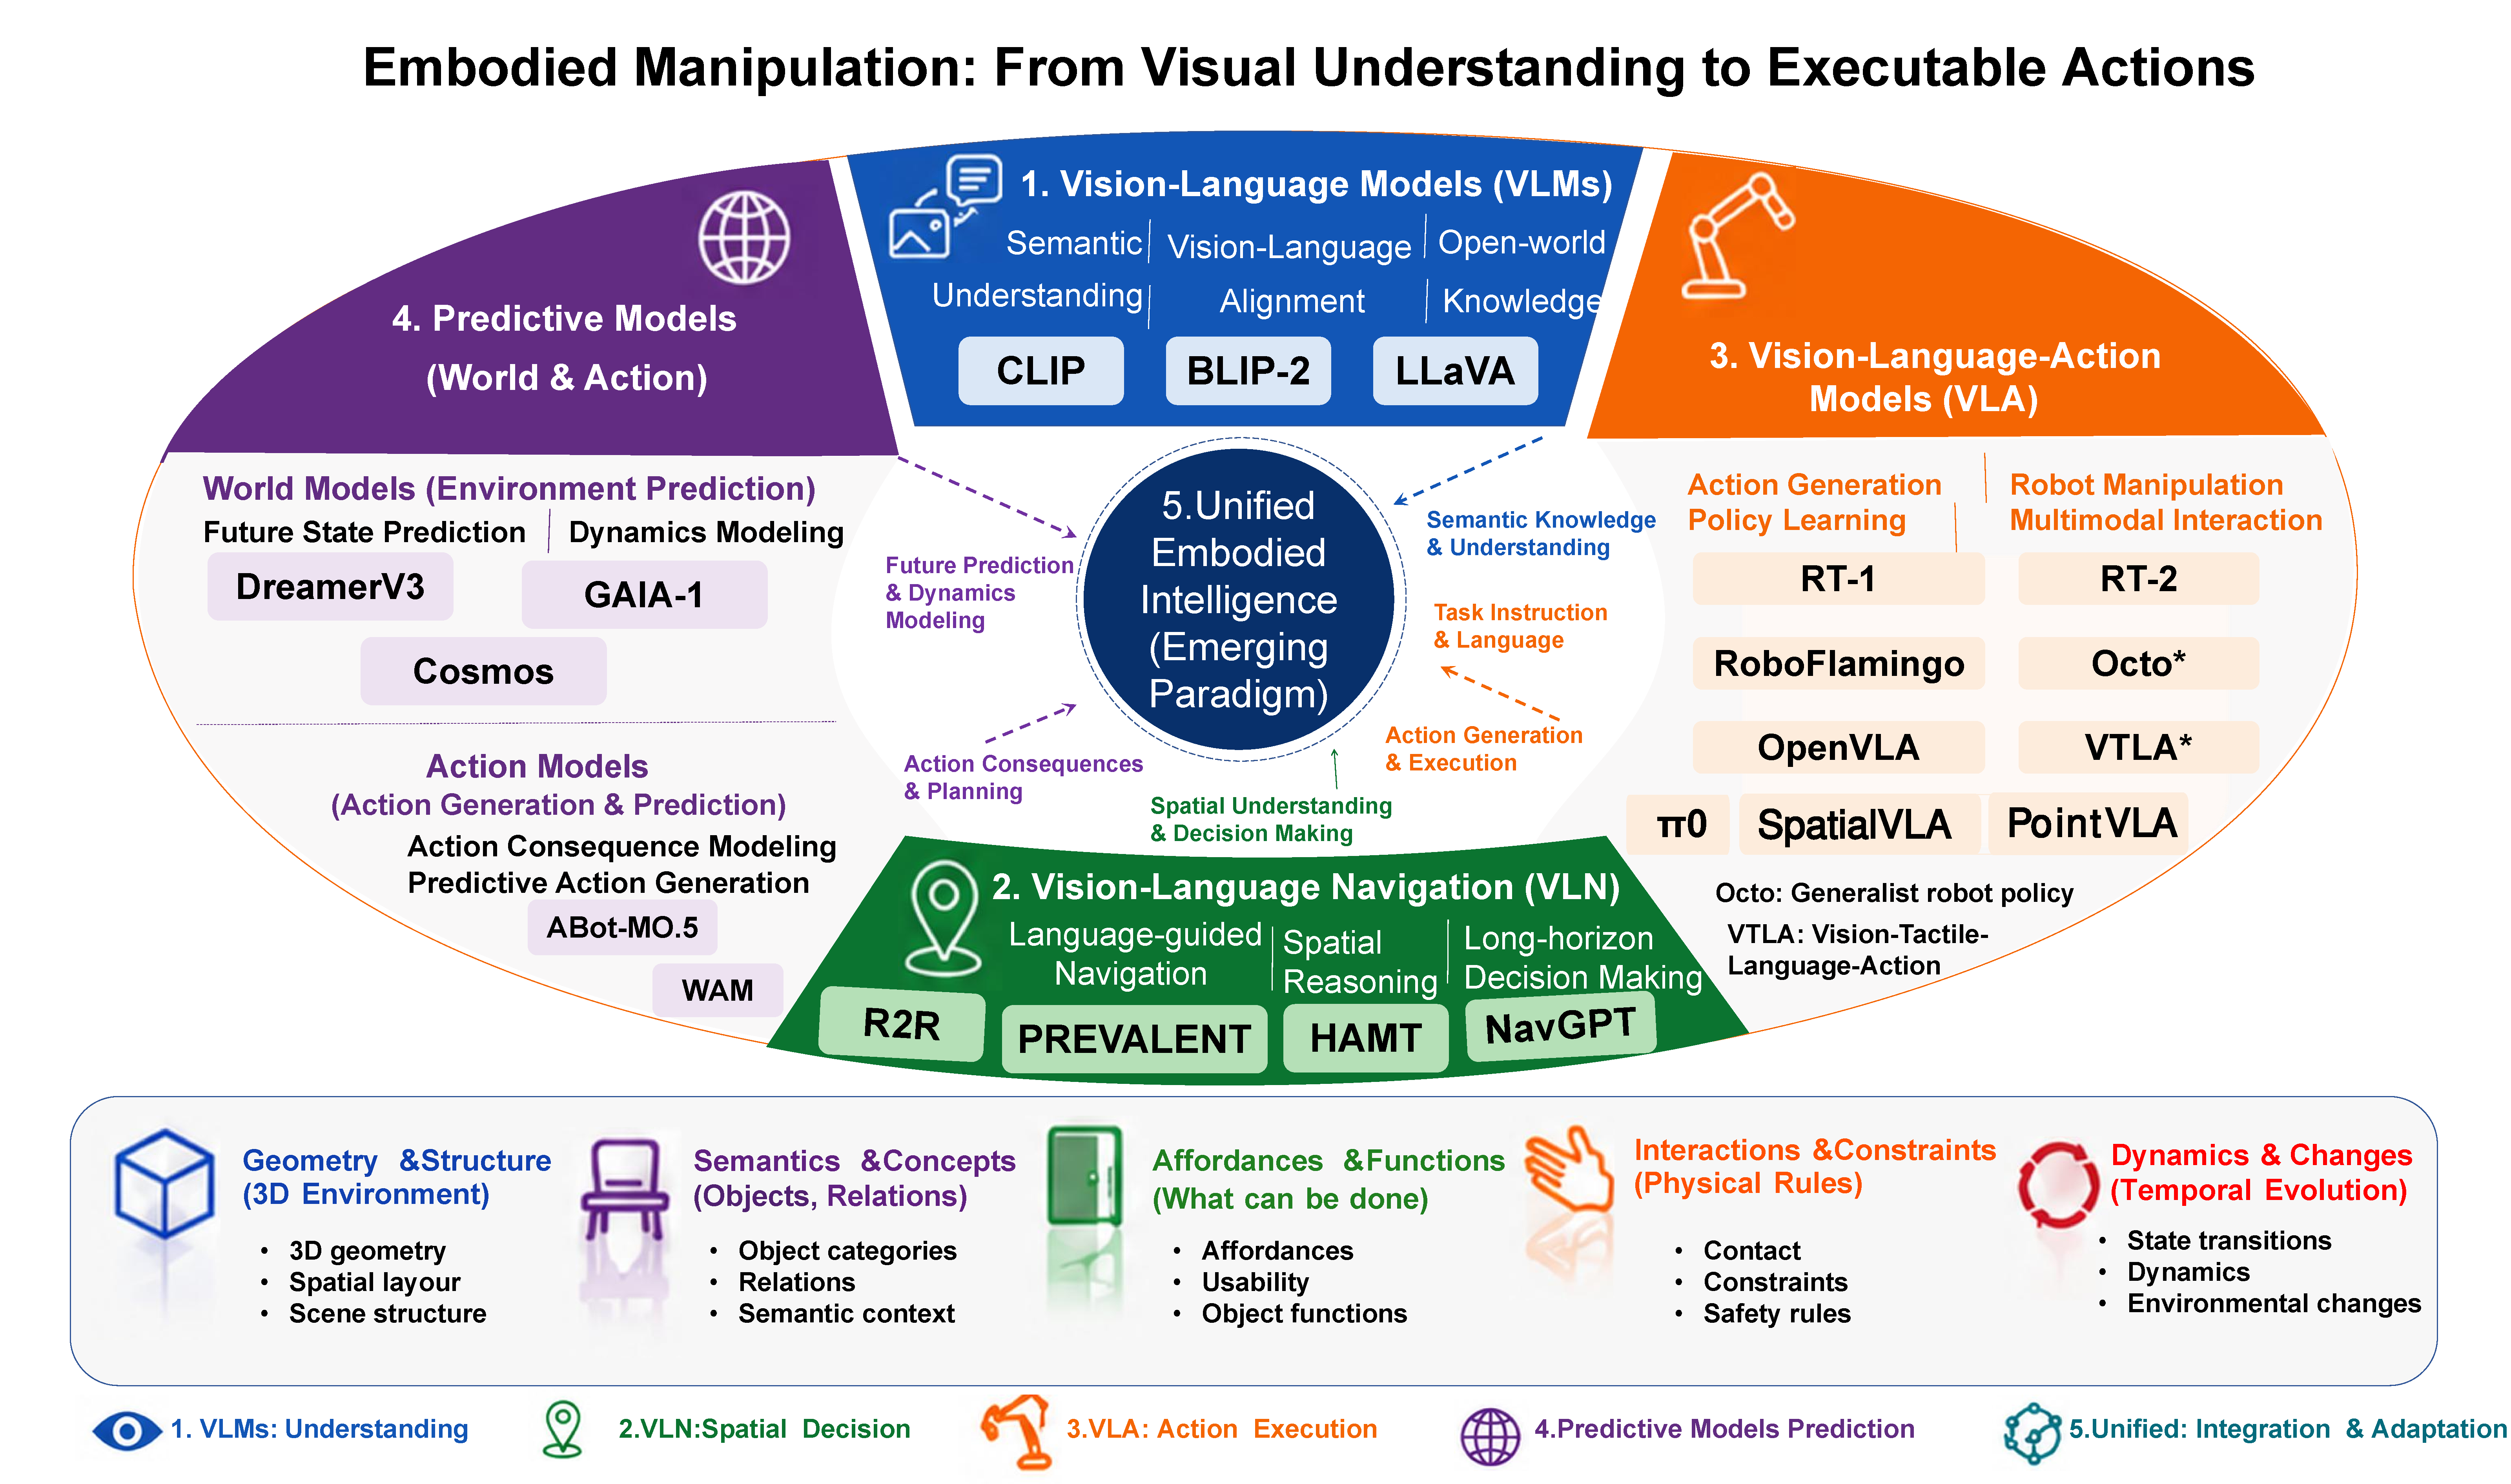
\includegraphics[width=\textwidth]{Figures/fig_embodied_intelligence.pdf}
\caption{
Taxonomy of representative paradigms in embodied intelligence. Existing approaches span vision-language understanding, language-guided navigation, vision-language-action execution, predictive world modeling, and unified embodied intelligence, providing complementary capabilities for semantic understanding, spatial reasoning, action generation, prediction, and physical interaction.
}
\label{fig:embodied_evolution}
\end{figure}
The preceding sections progressively construct an actionable representation of the environment, from geometric structure to semantic meaning and physical-functional properties. Geometric reconstruction provides the spatial structure of the scene; semantic understanding associates this structure with object identities, relations, and language-grounded meanings; and physical-functional understanding further characterizes the physical properties, affordances, and constraints that govern how objects can be interacted with. These representations are complementary layers of a common scene state rather than isolated outputs. Building on this unified scene representation, recent research on embodied manipulation has advanced along several complementary paradigms, including vision-language understanding, language-guided navigation, vision-language-action modeling, predictive world modeling, and unified embodied intelligence, as summarized in Fig.~\ref{fig:embodied_evolution}.

Executable embodied manipulation builds upon this scene state to transform perception and understanding into physical behavior. The central problem is not to replace geometric, semantic, or physical-functional representations with a single model, but to determine how these heterogeneous forms of scene knowledge can be accessed, reasoned over, and converted into reliable decisions and executable actions. From this perspective, vision-language models provide multimodal and language-grounded reasoning; vision-language navigation connects semantic goals with spatial decision making; vision-language-action models map task-conditioned observations to executable behavior; and world and action models introduce prediction of future states and action consequences before execution. Emerging unified embodied models increasingly couple these capabilities within shared architectures and closed-loop interaction.

Accordingly, this section organizes embodied manipulation according to four progressively coupled capabilities: \emph{multimodal scene reasoning}, which identifies task-relevant entities and interprets instructions in the context of the reconstructed scene; \emph{spatial and task-level decision making}, which connects goals with navigable regions, target objects, affordances, and task sequences; \emph{action generation and control}, which converts these decisions into executable behavior under geometric and physical constraints; and \emph{predictive modeling}, which anticipates future states and action consequences to support planning before execution. The final stage considers emerging unified embodied models that couple these capabilities while retaining the geometric, semantic, and physical-functional grounding established by the scene representation, as illustrated in Fig.~\ref{fig:embodied_unified_modeling}.
\subsection{Multimodal Scene Reasoning}
Vision-Language Models (VLMs) provide a semantic interface through which natural-language instructions can be associated with visual entities, attributes, and relations. Their importance to actionable scene understanding lies not in replacing geometric or physical representations, but in providing task-conditioned semantic grounding. Given an instruction, the model must identify which entities, regions, and relations in the scene are relevant to the intended action.

Early vision-language models established transferable visual-language representations through large-scale image-text pretraining. CLIP demonstrated that contrastive learning over web-scale image-text pairs can support open-vocabulary and zero-shot visual recognition~\cite{radford2021clip}. BLIP-2 and LLaVA subsequently integrated large language models with visual encoders, substantially extending multimodal question answering, instruction following, and visual reasoning~\cite{li2023blip,liu2023visual}. These models provide an important semantic interface for embodied agents, allowing natural-language goals to refer to objects, attributes, and relations beyond a fixed task vocabulary.

For embodied manipulation, however, semantic reasoning must remain grounded in the spatial and physical structure of the environment. Recognizing a ``drawer'' is insufficient: the agent must identify the correct instance, locate its actionable part, determine its articulation state, and establish whether the intended interaction is feasible. This motivates coupling VLMs with 3D scene representations, persistent spatial memory, and physical-functional information. Recent embodied foundation models increasingly incorporate spatial representations and robot-state information to bridge the gap between high-level multimodal semantics and low-level physical action, reflecting the persistent spatial and temporal mismatch between VLM representations and robot control spaces~\cite{zhen20243d}.

The resulting capability is therefore best understood as \emph{task-conditioned scene interpretation}. Language determines what is relevant to the task, while geometric and physical-functional representations determine where the relevant entities are and which interactions are feasible. This distinction is fundamental to embodied manipulation: semantic plausibility alone does not guarantee spatial correctness, physical feasibility, or executable behavior. Two failure modes make this gap concrete. First, VLMs are trained on 2D image--text statistics and can hallucinate absent objects~\cite{li2023pope}, misjudge distances and orientations, or produce semantically fluent but spatially wrong answers, and such errors propagate directly into embodied decisions. Second, VLM reasoning is usually evaluated on static question-answering benchmarks, which measure whether an answer is plausible in isolation rather than whether it leads to a correct action in the environment; temporal consistency across frames is rarely assessed at all.

\begin{figure}[t]
\centering
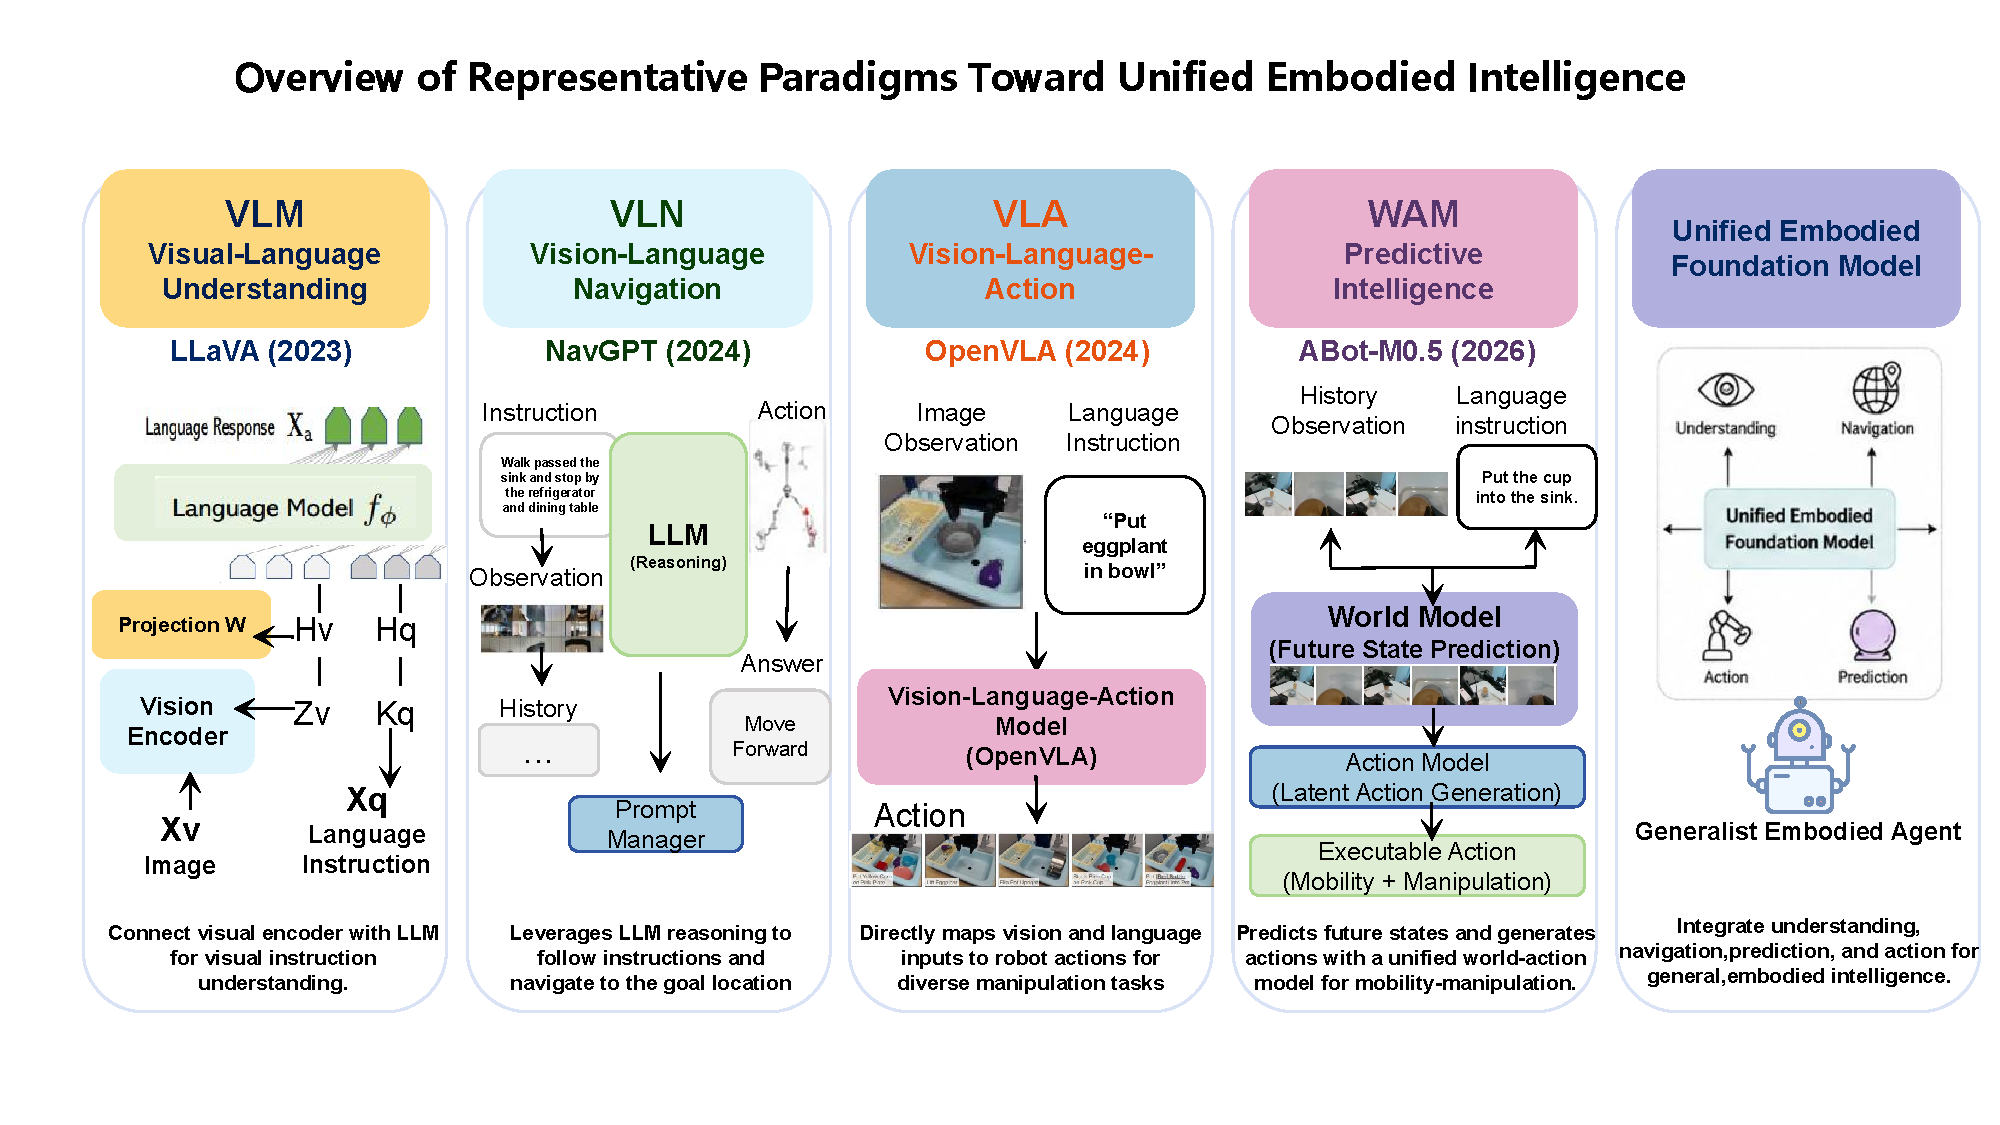
\includegraphics[width=\textwidth]{Figures/Embodied Unified Modeling.pdf}
\caption{
Overview of representative paradigms toward unified embodied intelligence. VLMs provide visual-language understanding, VLNs enable language-guided navigation, VLAs connect multimodal observations with executable actions, and world-action models introduce predictive modeling capabilities. These paradigms progressively converge toward unified embodied foundation models that integrate perception, reasoning, prediction, and action generation in closed-loop interaction.
}
\label{fig:embodied_unified_modeling}
\end{figure}
\subsection{Spatial and Task-Level Decision Making}
Once the scene has been interpreted in a task-relevant manner, the agent must determine where to move, which entities to approach, and how the task should be decomposed into executable subtasks. Spatial and task-level decision making therefore connects semantic goals with the navigable and manipulable structure of the environment.

Vision-language navigation (VLN) provides an early formulation of this capability by coupling natural-language instructions with sequential navigation decisions. The Room-to-Room (R2R) benchmark established a standard setting for instruction-guided navigation in indoor environments~\cite{anderson2018vision}. Subsequent methods introduced vision-language pretraining~\cite{hao2020towards}, historical trajectory modeling~\cite{chen2021history}, and language-model-based reasoning for instruction decomposition and navigation planning~\cite{zhou2024navgpt}. These developments progressively shifted navigation from local visual matching toward language-grounded spatial reasoning.

For complex indoor tasks, however, navigation is only one component of task-level decision making. An agent may need to locate an object, determine whether it is accessible, approach an appropriate interaction region, perform an operation, and subsequently navigate to another target. Navigation and manipulation are therefore successive decisions over a shared scene state rather than independent capabilities. Semantic maps, scene graphs, object-level spatial memory, and 3D scene representations provide intermediate structures through which task goals can be grounded into target entities, regions, and waypoints.

This perspective also exposes a limitation of conventional VLN: predicting a navigation trajectory does not by itself specify the task-level behavior required after reaching the target. Embodied decision making must jointly consider object identity, spatial configuration, affordances, task dependencies, and the current state of the environment. Recent embodied systems increasingly move toward hierarchical and memory-based decision making, in which high-level models generate task-relevant subgoals while lower-level policies execute them~\cite{ahn2022saycan}. Such decomposition is particularly important for long-horizon manipulation, where navigation, object selection, and interaction must be repeatedly interleaved. The evaluation setting reinforces the gap: most VLN benchmarks operate on static panoramic graphs, so they do not test continuous control under dynamic obstacles, nor whether the agent can perform any manipulation after arriving.~\cite{hong2021vln,savva2019habitat} Navigation success and task success are therefore conflated, and errors in hierarchical decomposition propagate downward---an incorrect subgoal can invalidate the entire subsequent execution even when each low-level skill is individually reliable.

\subsection{Action Generation and Control}
Action generation converts task-level decisions into physically executable behavior. Unlike semantic reasoning or navigation, which can tolerate some degree of abstraction, action generation must satisfy the geometric and physical constraints of the robot and its environment. It therefore represents the point at which scene representations are directly coupled to embodiment.

Vision-language-action (VLA) models provide a unified formulation by mapping multimodal observations and task instructions to robot actions. RT-1 demonstrated that large-scale, diverse robot datasets can support a generalist Transformer policy across multiple manipulation tasks~\cite{brohan2022rt}, while RT-2 transferred web-scale vision-language knowledge into robotic control and showed that semantic knowledge acquired from vision-language pretraining can improve task generalization~\cite{zitkovich2023rt}. Subsequent generalist policies, including Octo ~\cite{team2024octo} and OpenVLA ~\cite{kim2024openvla}, further explored scalable cross-task and cross-embodiment learning from heterogeneous robot demonstrations~\cite{team2024octo,kim2024openvla,openx2023openx}. $\pi_0$ extends this direction through a flow-based formulation for continuous robot action generation across diverse tasks and embodiments~\cite{team2024pi0}.

However, these models mainly rely on visual observations and implicit spatial representations, which can limit precise manipulation under complex geometric configurations. Recent studies therefore explore incorporating explicit spatial representations into VLA frameworks. SpatialVLA introduces spatially enhanced VLA modeling by integrating 3D positional encoding and adaptive spatial action representations, enabling stronger spatial understanding and improved generalization across robot setups~\cite{qu2025spatialvla}. PointVLA further injects point cloud representations into pretrained VLA models, allowing robots to exploit explicit 3D geometric information while preserving the benefits of large-scale vision-language pretraining~\cite{li2026pointvla}. These developments indicate a transition from purely vision-language conditioned action prediction toward spatially grounded and physically aware manipulation.


A key development is the increasing incorporation of additional spatial and physical signals. Purely image-based action prediction can be insufficient when successful execution depends on contact geometry, object articulation, material properties, or force-sensitive interaction. Accordingly, recent VLA research increasingly incorporates 3D representations, tactile observations~\cite{bi2026vla}, proprioception~\cite{wang2026think}, and dynamics-related priors~\cite{hu2023gaia} to improve action grounding and robustness. These developments reinforce the importance of the geometric and physical-functional representations established earlier: the action model does not operate on semantics alone, but requires spatially precise and physically meaningful inputs.

Despite their generality, current VLA models remain strongly dependent on the distribution and quality of robot interaction data. Imitation learning provides effective supervision for frequently demonstrated behaviors, but it offers limited information about actions that were not observed, especially under novel object configurations or dynamics. A policy may therefore generate a plausible action while lacking a reliable estimate of whether that action will succeed. At a deeper level, imitation learns observation--action correlations rather than a causal model of success, so failures under distribution shift are not detected by the policy itself, and success-rate evaluation can mask brittle behaviors that exploit incidental cues in the demonstration distribution. The bottleneck is often representational rather than algorithmic: grasp points, contact poses, and articulated-state estimates must be precise at the millimeter level, so the quality of the scene representation directly bounds what even a well-trained action model can achieve. This limitation motivates predictive modeling as a complementary capability rather than as a replacement for action generation.

\subsection{Predictive Modeling}
Action generation determines what the agent intends to do, whereas predictive modeling estimates what may happen if that action is executed. This distinction is fundamental for long-horizon embodied behavior because many actions have consequences that cannot be assessed from the current observation alone.

World models provide a general framework for learning compact representations of environmental dynamics and predicting future states under candidate actions. Early formulations established the principle of learning latent environment models for planning and imagination~\cite{ha2018world}, while DreamerV3 demonstrated scalable latent-dynamics learning and imagination-based decision making across diverse environments~\cite{hafner2023mastering}. More recent generative world models extend prediction toward visually rich and controllable environments~\cite{brooks2024video}, including Genie for interactive environments~\cite{bruce2024genie} and GAIA-1 for generative world modeling in driving scenarios~\cite{hu2023gaia}.

For embodied manipulation, however, visual plausibility alone is insufficient. A useful predictive model must preserve the state variables that determine interaction outcomes, including object motion, contact relations, articulation, and task-relevant physical constraints. The prediction target is therefore not limited to future visual observations, but should capture scene states that support downstream decision making. Recent work on physical world modeling explores this direction by jointly modeling multimodal 3D scene information, including RGB observations, optical flow, and camera motion, within a unified framework. Such models support multiple inference tasks, including depth estimation, novel view synthesis, and object manipulation, demonstrating the potential of predictive models to capture both visual and physical aspects of the environment ~\cite{lee2026unified}. 

Action models complement world models by explicitly linking predicted environmental states to candidate behaviors. Rather than merely forecasting what the environment may look like, an action-conditioned model evaluates how different actions may alter the scene and which resulting states are desirable under a task objective. Recent embodied systems increasingly combine mobility and manipulation within a shared predictive framework, illustrating a broader trend toward planning over future states rather than selecting actions solely from the current observation~\cite{chen2026abot}.

Nevertheless, predictive modeling remains challenging in real environments. Long-horizon predictions accumulate error, partially observed states are inherently ambiguous, and contact-rich interactions can produce discontinuous state transitions. Moreover, visually plausible predictions may violate physical constraints even when their appearance remains convincing~\cite{kang2024far}. A further mismatch concerns evaluation: prediction models are typically judged by reconstruction or visual fidelity, which is only weakly related to decision quality. A prediction that is slightly less accurate visually but preserves the decision-relevant state variables---contact relations, object permanence, stability---is more useful for planning than a visually faithful one that violates them, yet standard metrics cannot distinguish the two. Uncertainty estimates are likewise rarely propagated into the decision maker, so the planner cannot tell which predictions it should trust. Consequently, predictive modeling should be coupled with the physical-functional representation and consistency constraints established earlier, so that future-state prediction remains grounded in the underlying scene structure.
\begin{table}[!tbp]
\centering

\caption{
Taxonomy of Embodied Intelligence: From Visual Understanding to Executable Actions
}

\label{tab:embodied_taxonomy}

\footnotesize

\setlength{\tabcolsep}{3pt}
\renewcommand{\arraystretch}{1.3}

\rowcolors{2}{TableSub}{white}

\begin{tabularx}{\textwidth}{
>{\centering\arraybackslash}p{2.1cm}
>{\centering\arraybackslash}p{2.2cm}
>{\centering\arraybackslash}p{3.0cm}
>{\centering\arraybackslash}X
>{\centering\arraybackslash}X
}

\toprule

\rowcolor{TableNavy}

\textcolor{white}{\textbf{Paradigm}}
&
\textcolor{white}{\textbf{Core Objective}}
&
\textcolor{white}{\textbf{Representative Works}}
&
\textcolor{white}{\textbf{Main Capabilities}}
&
\textcolor{white}{\textbf{Remaining Challenges}}
\\

\midrule

\textbf{Vision-Language Models (VLMs)}
&
Semantic understanding
&
CLIP ~\cite{radford2021clip}, 
BLIP-2 ~\cite{li2023blip}, 
LLaVA ~\cite{liu2023visual}
&
Vision-language alignment, open-world recognition, multimodal reasoning, semantic knowledge transfer
&
Limited 3D grounding, weak physical understanding, and insufficient interaction reasoning
\\

\textbf{Vision-Language Navigation (VLN)}
&
Language-guided spatial decision making
&
R2R ~\cite{anderson2018vision}, 
PREVALENT ~\cite{hao2020towards}, 
HAMT ~\cite{chen2021history}, 
NavGPT ~\cite{zhou2024navgpt}
&
Instruction following, spatial reasoning, historical trajectory modeling, and long-horizon navigation
&
Ambiguous instructions, accumulated navigation errors, incomplete observations, and adaptation to dynamic environments
\\

\textbf{Vision-Language-Action (VLA) Models}
&
Multimodal perception-to-action mapping
&
RT-1 ~\cite{brohan2022rt}, 
RT-2 ~\cite{zitkovich2023rt}, 
RoboFlamingo ~\cite{li2024vision}, 
Octo ~\cite{team2024octo}, 
OpenVLA ~\cite{kim2024openvla}, 
$\pi_0$ ~\cite{team2024pi0},
VTLA ~\cite{zhang2026vtla},
SpatialVLA ~\cite{qu2025spatialvla},
PointVLA ~\cite{li2026pointvla}
&
Robot action generation, imitation learning, task generalization, cross-embodiment transfer, and multimodal physical interaction
&
High cost of robot data, distribution shift, limited physical reasoning, and unreliable long-horizon execution
\\

\textbf{World and Action Models}
&
Predicting environmental evolution and action consequences
&
World Models ~\cite{ha2018world}, 
DreamerV3 ~\cite{hafner2023mastering}, 
GAIA-1 ~\cite{hu2023gaia}, 
Genie ~\cite{bruce2024genie}, 
ABot-M0.5 ~\cite{chen2026abot}
&
Latent dynamics modeling, future-state prediction, imagination-based planning, action-conditioned prediction, and mobility-manipulation coordination
&
Long-horizon prediction accuracy, physical consistency, action grounding, and real-world robustness
\\

\midrule

\textbf{Unified Embodied Intelligence}
&
Cross-paradigm integration
&
Emerging integration of multimodal understanding, action generation, and predictive modeling
&
Joint use of semantic reasoning, spatial understanding, physical interaction, environmental prediction, and feedback
&
No established unified architecture, high data and computation requirements, safety, and generalization in open environments
\\

\bottomrule

\end{tabularx}

\end{table}
\subsection{Unified Embodied Modeling}
The capabilities discussed above are increasingly integrated into unified embodied models (Table~\ref{tab:embodied_taxonomy}). The objective of this integration is not to collapse geometric, semantic, physical, and functional knowledge into an undifferentiated latent space, but to allow these complementary forms of information to be jointly accessed throughout the behavioral loop. A unified model should therefore preserve the distinct roles of scene representation, task reasoning, action generation, and future-state prediction while enabling information to flow between them.

Early efforts such as 3D-VLA explicitly incorporate 3D scene structure into vision-language-action modeling, demonstrating that spatial representations can provide stronger grounding for embodied reasoning and action generation~\cite{zhen20243d}. More recent physical-world foundation models, including Cosmos~\cite{agrawal2025cosmos}, aim to provide scalable visual and physical representations for Physical AI, serving as general-purpose infrastructure for downstream prediction, planning, and control rather than constituting complete embodied agents by themselves. The broader trend is toward models that jointly process visual observations, language, spatial structure, actions, and predicted future states.

This integration creates an important shift in system design. Instead of passing information through a fixed sequence of isolated modules, unified embodied models can maintain shared task-conditioned representations in which scene understanding informs decision making, physical constraints shape action generation, and predicted consequences influence subsequent choices. Such coupling can improve knowledge transfer across tasks and reduce the interface mismatch between perception, planning, and control. At the same time, tighter coupling also propagates errors: an incorrect object grounding can affect planning, an inaccurate physical estimate can lead to unsafe actions, and an erroneous future prediction can bias subsequent decisions.

The resulting framework is therefore better understood as a \emph{closed-loop integration of complementary capabilities} rather than a single monolithic model. Geometric representations provide spatial grounding; semantic representations provide object, relational, and linguistic meaning; physical-functional representations provide affordances and interaction constraints; multimodal reasoning identifies task-relevant information; decision making selects goals and behaviors; action models execute these decisions; and predictive models evaluate possible future states. The integration of these components transforms the actionable scene representation from a static description into a state that can participate directly in embodied behavior.

A major challenge is determining how much of this knowledge should be represented explicitly and how much should be learned implicitly within a foundation model. Explicit geometric and physical representations offer interpretability, controllability, and consistency checks, whereas large multimodal models provide flexible semantic reasoning and broad generalization. Future embodied systems are therefore likely to combine structured scene representations with large learned models rather than relying exclusively on either paradigm~\cite{driess2023palme}. The closed-loop nature of these systems amplifies this difficulty: unlike modular pipelines, where errors can be contained within a stage, unified models propagate errors across perception, reasoning, and action, so a small grounding mistake can bias planning and execution in ways that are difficult to attribute. There is also no standardized benchmark that jointly exercises perception, decision, action, and prediction in a physically consistent loop, which makes system-level progress hard to measure and hard to compare across architectures. Equally important are long-horizon evaluation, physical consistency, data efficiency, and robustness to unseen environments, which remain critical requirements for reliable deployment.

Overall, embodied unified modeling completes the progression from geometric reconstruction to semantic understanding, physical-functional reasoning, and embodied action. The resulting system does not discard the preceding representations; instead, it connects them through perception, decision making, action, and prediction, allowing geometric structure, semantic meaning, and physical-functional knowledge to jointly constrain behavior. This provides the foundation for reliable embodied manipulation in complex indoor environments, although the reliability of the whole is bounded by its weakest link: no current architecture jointly maintains the geometric precision, physical validity, temporal persistence, and task-level reasoning that actionability requires. Meeting these requirements jointly, rather than optimizing each capability in isolation, is precisely the challenge addressed in the next section.

\section{Conclusion and Future Directions}
\label{sec:conclusion}


\begin{figure}[!t]
    \centering
    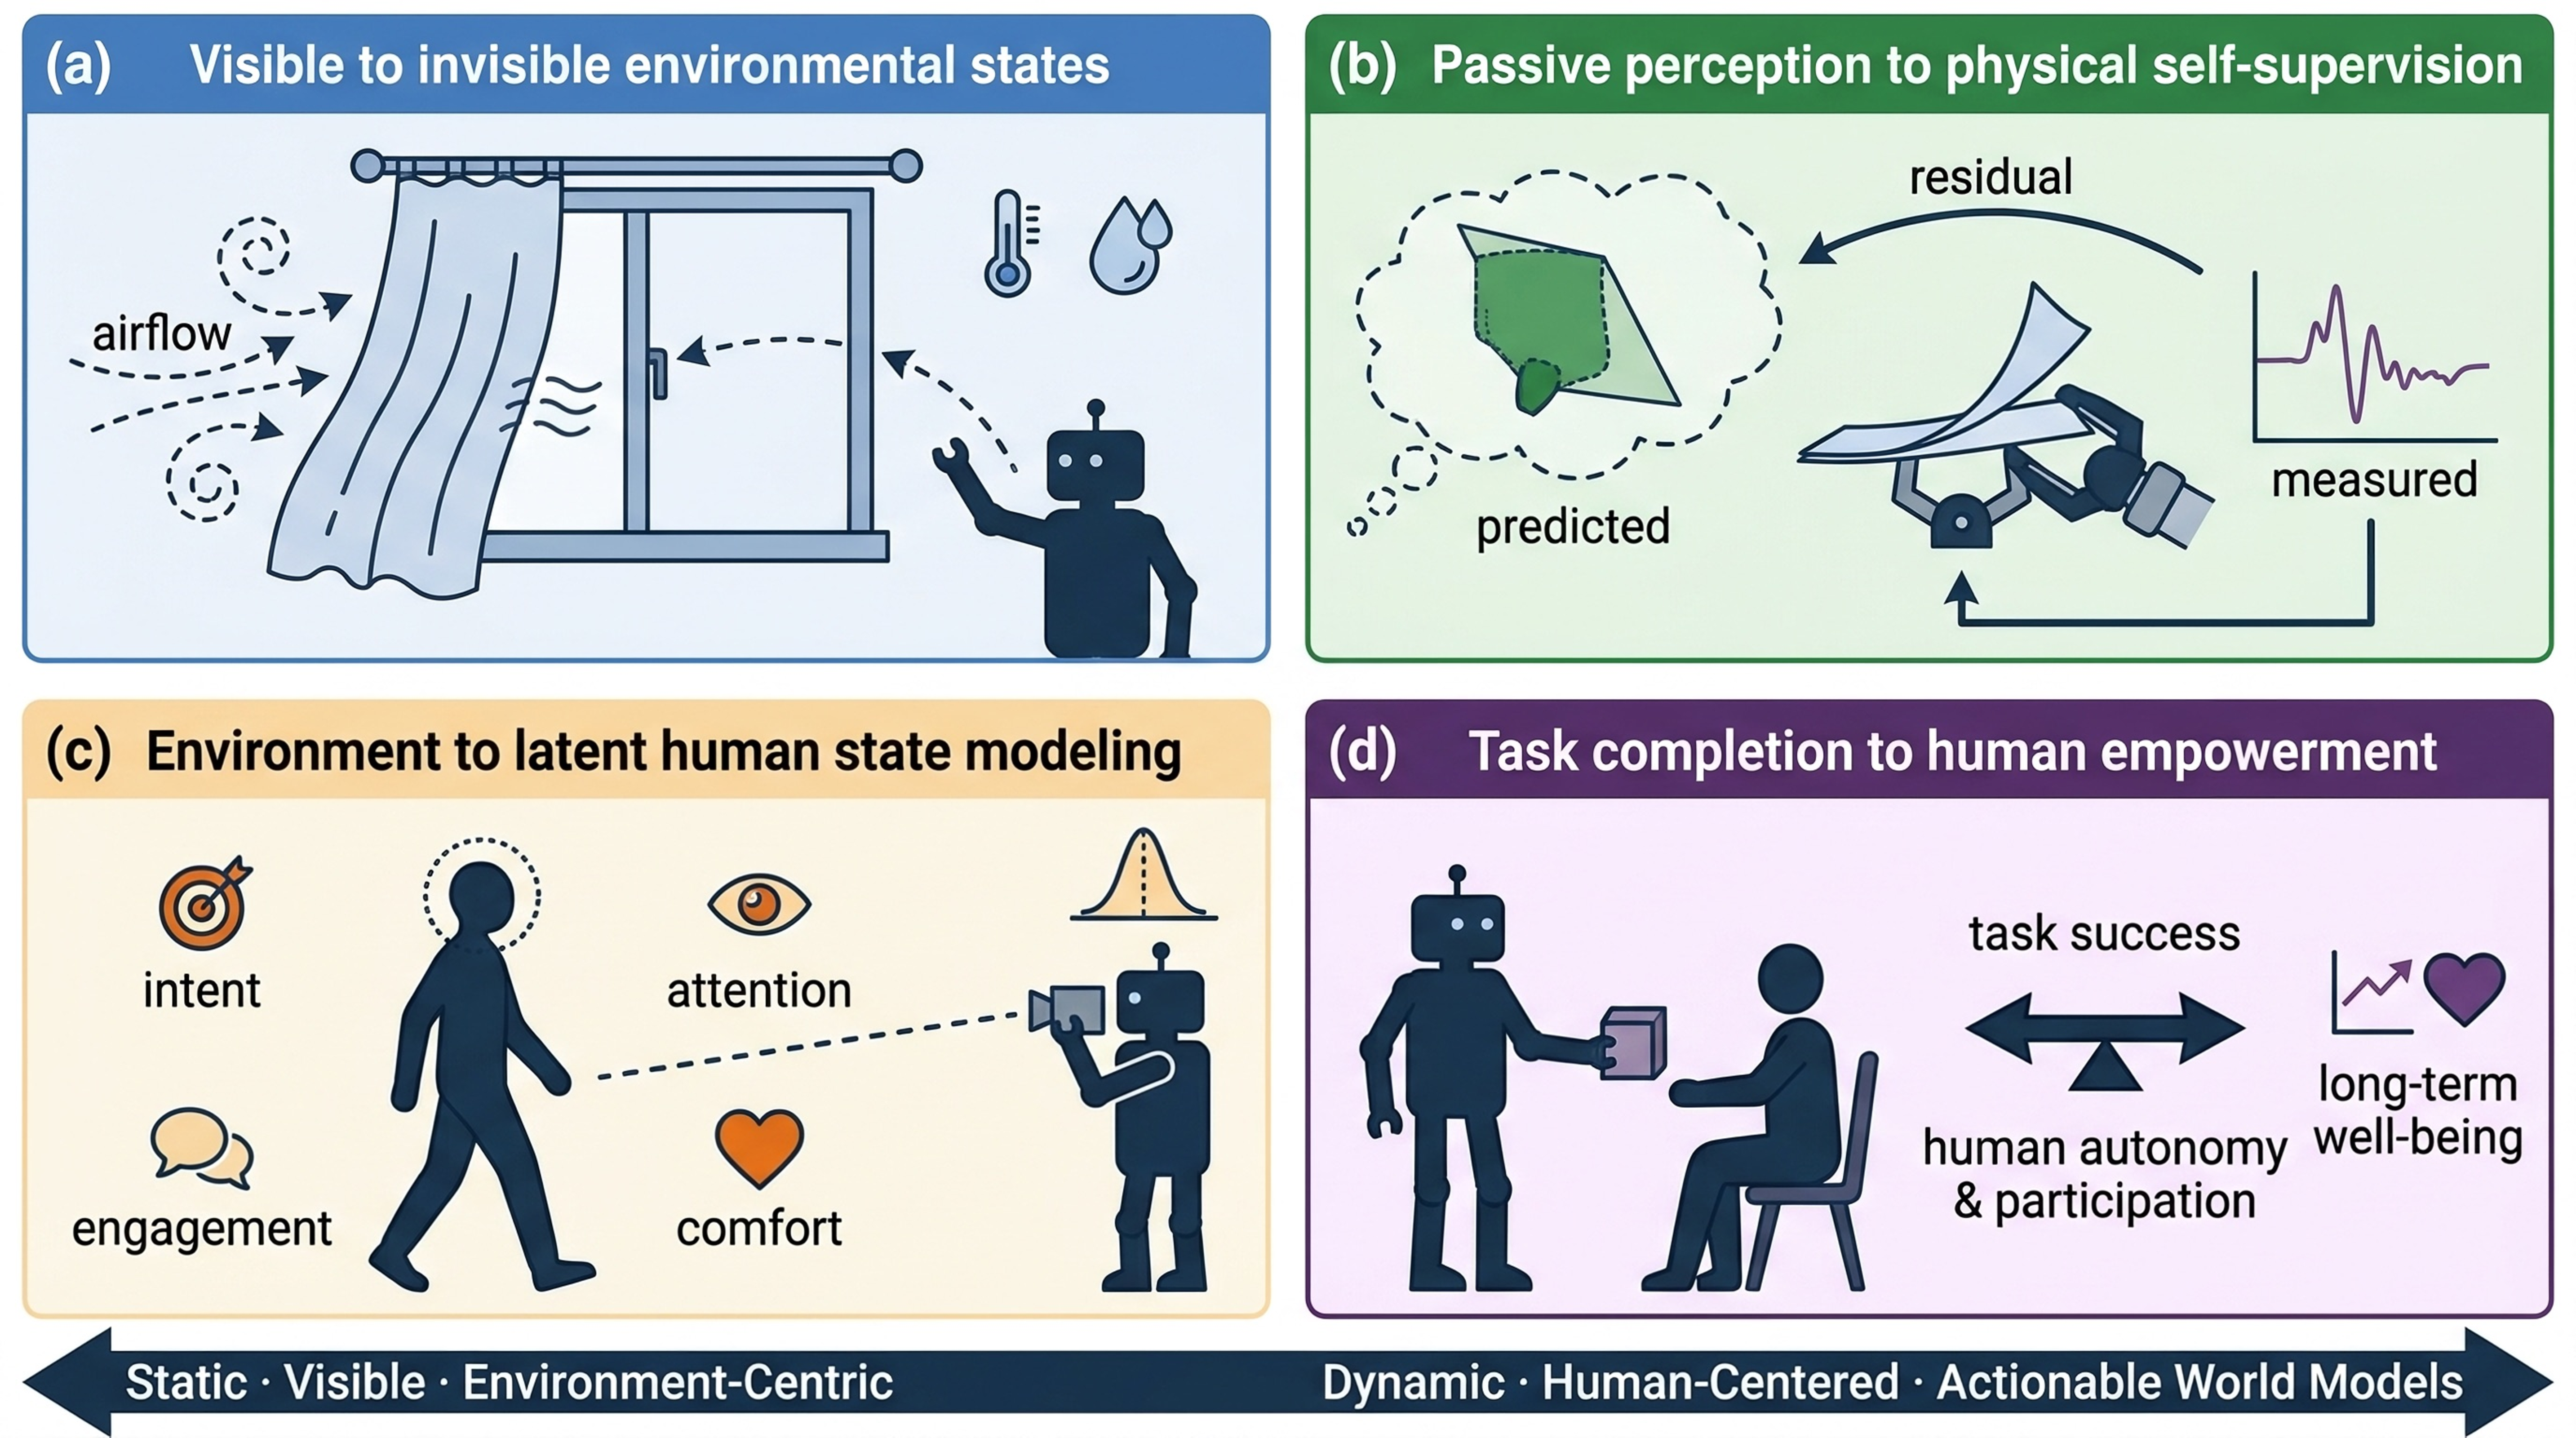
\includegraphics[width=\linewidth]{Figures/fig_future_directions.pdf}
    \caption{Four future directions for embodied indoor scene understanding:
(a) from visible reconstruction to inference of latent environmental states;
(b) from passive perception to physically grounded self-supervision;
(c) from environment-centric modeling to human-state-aware scene understanding; and
(d) from task-oriented execution to human-centered embodied intelligence.
Together, these directions shift indoor scene modeling toward dynamic, physically grounded, and human-centered representations that support reliable embodied behavior.}
    \label{fig:future_directions}
\end{figure}

\subsubsection{Summary of Key Advances}
This survey has organized the evolution of indoor scene modeling around four progressively coupled capabilities: geometric reconstruction, semantic understanding, physical-functional understanding, and embodied unified modeling. Together, they trace a transition from recovering the spatial structure of an environment to building representations that can support interpretation, interaction, and executable behavior.

Geometric reconstruction has evolved from classical SLAM and multiview reconstruction toward neural implicit and Gaussian-based representations, enabling increasingly dense, scalable, and temporally adaptive modeling. Semantic understanding has correspondingly progressed from object-level recognition and segmentation to open-vocabulary perception, relational scene modeling, layout reasoning, and geometry--semantic integration, allowing reconstructed environments to be interpreted as structured scenes rather than collections of independent surfaces. Physical-functional understanding further grounds these representations in the properties, affordances, and constraints that determine how objects can be manipulated. Building on these layers, large-model-driven embodied modeling increasingly couples multimodal reasoning, spatial decision making, action generation, and predictive modeling, providing a pathway from scene understanding to executable embodied behavior.

Taken together, these developments indicate a fundamental shift in the role of indoor scene reconstruction: from recovering \emph{what is present} to maintaining a structured scene state that supports \emph{what can be understood, what can be done, and how actions should be executed}. Nevertheless, current systems still struggle to maintain such representations under partial observability, dynamic changes, physical uncertainty, and long-horizon tasks. Bridging this gap requires scene representations that are not only geometrically and semantically accurate, but also physically grounded, temporally persistent, and directly coupled with embodied decision making. The following subsection discusses the key challenges and future research directions toward this goal.

\subsubsection{Open Challenges and Research Opportunities}

We identify four directions (Fig.~\ref{fig:future_directions}) that may shape the next stage of actionable scene understanding for embodied manipulation. Together, they extend scene understanding from visible geometry to latent physical states, from passive observation to interaction-driven updating, and from robot-centric task execution to human-aware manipulation.

\paragraph{From Visible Reconstruction to Latent Physical-State Inference}
Current scene representations primarily describe observable geometry, semantics, and physical properties. However, successful manipulation also depends on latent states such as airflow, temperature, internal deformation, friction, and subtle environmental disturbances. A promising direction is to infer such states from their observable effects, including object motion, deformation, and vibration, and to continuously update their estimates as new observations arrive. This would enable robots to anticipate manipulation-relevant changes rather than react only after they become observable.

\paragraph{From Passive Perception to Interaction-Driven Scene Updating}
Scene understanding should not remain a one-time perception process. During manipulation, contact, force, and tactile feedback provide direct evidence about object properties and interaction states that vision alone cannot reliably determine. Future systems should therefore use interaction outcomes to update geometry, physical properties, affordances, and manipulation strategies online, turning physical interaction into a source of self-supervision for actionable scene understanding.

\paragraph{From Object-Centered Modeling to Human-Aware Scene Understanding}
Indoor manipulation frequently occurs around people, whose intentions, attention, activity, and preferences influence what actions are appropriate. Beyond modeling objects and their physical states, actionable scene understanding should therefore incorporate temporally accumulated and uncertainty-aware representations of human states that are directly relevant to manipulation. This shift would enable robots to select actions that are not only physically feasible, but also contextually appropriate and responsive to human presence.

\paragraph{From Task Success to Human-Centered Actionability}
Task completion alone is insufficient to characterize the quality of embodied manipulation. A robot may complete a task while unnecessarily restricting human participation or autonomy. Future evaluation should therefore consider not only execution success and efficiency, but also whether actions preserve appropriate human involvement and support long-term human--robot collaboration~\cite{puig2021watch}. This calls for actionability metrics that jointly assess physical feasibility, task effectiveness, and human-centered outcomes.

Together, these directions point toward a broader goal: evolving actionable scene understanding into an emotion- and intention-aware representation that enables embodied manipulation to effectively serve human needs.
%%%%%%%%%%%%%%%%%%%%%%%%%%%%%%%%%%%%%%%%%%%%%%%%%%%%%%%
%%% Reference section.
%%%%%%%%%%%%%%%%%%%%%%%%%%%%%%%%%%%%%%%%%%%%%%%%%%%%%%%
\bibliographystyle{scis}
\bibliography{ref}

\end{document}
